% example for dissertation.sty
\documentclass[
  % Replace oneside by twoside if you are printing your thesis on both sides
  % of the paper, leave as is for single sided prints or for viewing on screen.
  oneside,
  %twoside,
  11pt, a4paper,
  footinclude=true,
  headinclude=true,
  cleardoublepage=empty
]{scrbook}

\usepackage{dissertation}
 
\theoremstyle{definition}
\newtheorem{definition}{Definition}[section]
 
\theoremstyle{definition}
\newtheorem{example}{Example}[definition]
 
\newtheorem{theorem}{Theorem}[section]
\newtheorem{corollary}{Corollary}[theorem]

\usepackage{upgreek}
%----- jno added stuff -----
%\usepackage{fleqn}
%\setlength\mathindent{3em}
\usepackage{multirow}
\usepackage{amssymb}
\newenvironment{lcbr}{\left\{\begin{array}{l}}{\end{array}\right.}
\usepackage[all]{xy}
\def\rarrow#1#2#3{\def\nolabel{}\def\lab{#2}\ifx\lab\nolabel{#1\to #3}\else\xymatrix{ #1 \ar[r]^-{#2} & #3 }\fi}
\def\larrow#1#2#3{\def\nolabel{}\def\lab{#2}\ifx\lab\nolabel{#3\from#1}\else\xymatrix{ #3 & #1 \ar[l]_-{#2}}\fi}
\def\longlarrow#1#2#3{\xymatrix{ #3 && #1 \ar[ll]_-{#2} }}
\def\longrarrow#1#2#3{\xymatrix{ #1 \ar[rr]^-{#2} && #3 }}
\usepackage{wrapfig}
\def\doc{paper}
\def\start{&&}
\def\more{\\&&}
\def\just#1#2{\\ &#1& \rule{2em}{0pt} \{ \mbox{\rule[-.7em]{0pt}{1.8em} \small #2 \/} \} \nonumber\\ && }
\def\conv#1{#1^\circ}
\def\comp{ \mathbin{\cdot} }
\def\kr{\mathbin{\hbox{\tiny${}^\triangledown$}}}
\let\kons=\underline
\def\xsor{{\dot\vee}}
%-----
\def\msplit#1#2{\left[\begin{array}{c}#1\\\hline#2\end{array}\right]} % Split
\def\meither#1#2{\left[\begin{array}{c|c}{#1}&{#2}\end{array}\right]} % either
\def\matfour#1#2#3#4{\begin{bmatrix} \left.\begin{matrix} \dfrac{#1}{#3} \end{matrix}\ \right|\ \begin{matrix} \dfrac{#2}{#4} \end{matrix}\end{bmatrix}}
%------
\def\grantsponsor#1#2#3{#2}
\newcommand\grantnum[3][]{#3%
  \def\@tempa{#1}\ifx\@tempa\@empty\else\fi}
%---------------------------

% ACRONYMS -----------------------------------------------------

%import the necessary package with some options
%\usepackage[acronym,nonumberlist,nomain]{glossaries}

%enable the following to avoid links from the acronym usage to the list
%\glsdisablehyper

%displays the first use of an acronym in italic
\defglsdisplayfirst[\acronymtype]{\emph{#1#4}}

%the style of the Glossary
\glossarystyle{listgroup}

% set the name for the acronym entries page
\renewcommand{\glossaryname}{Acronyms}

%this shall be the last thing in the acronym configuration!!
\makeglossaries

% here are the acronym entries
\newacronym{miei}{MIEI}{Integrated Master in Computer Engineering}
\newacronym{di}{DI}{Informatics Department}
\newacronym{um}{UM}{University of Minho}
\newacronym{fp}{FP}{Functional Programming}
\newacronym{ct}{CT}{Category Theory}
\newacronym{cs}{CS}{Computer Science}
\newacronym{pfp}{PFP}{Probabilistic Functional Programming}
\newacronym{aop}{AoP}{Algebra of Programming}
\newacronym{laop}{LAoP}{Linear Algebra of Programming}
\newacronym{saf}{SAF}{Selective Applicative Functors}
\newacronym{edsl}{eDSL}{Embedded domain specific language}
\newacronym{ppl}{PPL}{Probabilistic Programming Language}
\newacronym{gadt}{GADT}{Generalised Algebraic Datatype}
\newacronym{ghc}{GHC}{Glasgow Haskell Compiler}

% these could go in an acronyms.tex file, and loaded with:
% \loadglsentries[\acronymtype]{Parts/Definitions/acronyms}
% when using this, you may want to remove 'nomain' from the package options

%% **MORE INFO** %%

%to add the acronyms list add the following where you want to print it:
%\printglossary[type=\acronymtype]
%\clearpage
%\thispagestyle{empty}

%to use an acronym:
%\gls{qps}

% compile the thesis in command line with the following command sequence:
% pdlatex dissertation.tex
% makeglossaries dissertation
% bibtex dissertation
% pdlatex dissertation.tex
% pdlatex dissertation.tex

% ----------------------------------------------------------------

% Title
\titleA{Selective Applicative Functors}
\titleB{\& Probabilistic Programming} % (if any)
%\subtitleA{First Part of Subtitle}
%\subtitleB{Second part of Subtitle} % (if any)

% Author
\author{Armando João Isaías Ferreira dos Santos}

% Supervisor(s)
\supervisor{José Nuno Oliveira (INESCTEC \& University of Minho)} %Mudar o bold
\cosupervisor{Andrey Mokhov (Newcastle University, UK)}

% University (uncomment if you need to change default values)
% \def\school{Escola de Engenharia}
% \def\department{Departamento de Inform\'{a}tica}
% \def\university{Universidade do Minho}
% \def\masterdegree{Computer Science}

% Date
\date{\myear} % change to text if date is not today

% Keywords
%\keywords{master thesis, functional programming, probabilistic programming, monads, applicatives, selective applicative functor, haskell}

% Glossaries & Acronyms
%\makeglossaries  %  either use this ...
%\makeindex	   % ... or this

% Define Acronyms
%%!TEX root = ../dissertation.tex

\newacronym{mei}{MEI}{Mestrado em Engenharia Inform\'{a}tica}
\newacronym{um}{UM}{Universidade do Minho}
%\glsaddall[types={\acronymtype}]



\ummetadata % add metadata to the document (author, publisher, ...)

\begin{document}
	% Cover page ---------------------------------------
	\umfrontcover	
	\umtitlepage
	
	% Add acknowledgements ----------------------------
	\chapter*{Acknowledgements}
	Acknowledgements to be written here. %Agradecer ao prof. Andrey

	% Add abstracts (en,pt) ---------------------------
	\chapter*{Abstract}

    In functional programming, \emph{selective applicative} functors (SAF) are an abstraction between applicative functors and monads. This abstraction requires all effects to be statically declared, but provides a way to select which effects to execute dynamically. SAF have been shown to be a useful abstraction in several examples, including two industrial case studies. Selective functors have been used for their static analysis capabilities. The collection of information about all possible effects in a computation and the fact that they enable \emph{speculative} execution make it possible to take advantage to describe probabilistic computations instead of using monads. In particular, selective functors appear to provide a way to obtain a more efficient implementation of probability distributions than monads.
    
    This dissertation addresses a probabilistic interpretation for the \emph{arrow} and \emph{selective} abstractions in the light of the linear algebra of programming discipline, as well as exploring ways of offering SAF capabilities to probabilistic programming, by exposing sampling as a concurrency problem. As a result, provides a Haskell type-safe matrix library capable of expressing probability distributions and probabilistic computations as typed matrices, and a probabilistic programming eDSL that explores various techniques in order to offer a novel, performant solution to probabilistic functional programming.
	
	\vskip0.5cm
    \keywords{master thesis, functional programming, probabilistic programming, monads, applicatives, selective applicative functor, Haskell, matrices}
	
	\cleardoublepage
	\chapter*{Resumo}
	
	%Este documento descreve o trabalho realizado até o momento no projeto de mestrado "Selective Applicative Functors \& Probabilistic Programming".
    
    Em programação funcional, os functores \emph{aplicativos seletivos} (FAS) são uma abstração entre functores aplicativos e monades. Essa abstração requer que todos os efeitos sejam declarados estaticamente, mas fornece uma maneira de selecionar quais efeitos serão executados dinamicamente. FAS têm se mostrado uma abstração útil em vários exemplos, incluindo dois estudos de caso industriais. Functores seletivos têm sido usados pela suas capacidade de análise estática. O conjunto de informações sobre todos os efeitos possíveis numa computação e o facto de que eles permitem a execução \emph{especulativa} tornam possível descrever computações probabilísticas. Em particular, functores seletivos parecem oferecer uma maneira de obter uma implementação mais eficiente de distribuições probabilisticas do que monades.
        
    Esta dissertação aborda uma interpretação probabilística para as abstrações \emph{Arrow} e \emph{Selective} à luz da disciplina da álgebra linear da programação, bem como explora formas de oferecer as capacidades dos FAS para programação probabilística, expondo \emph{sampling} como um problema de concorrência. Como resultado, fornece uma biblioteca de matrizes em Haskell, capaz de expressar distribuições de probabilidade e cálculos probabilísticos como matrizes tipadas e uma eDSL de programação probabilística que explora várias técnicas, com o obejtivo de oferecer uma solução inovadora e de alto desempenho para a programação funcional probabilística.
	
	\vskip0.5cm
    \keywordsPT{dissertação de mestrado, programação funcional, programação probabilística, monades, aplicativos, funtores aplicativos seletivos, haskell, matrizes}
    
	% Summary Lists ------------------------------------
	\tableofcontents
	\listoffigures
	\listoftables
	\lstlistoflistings
	%\listofabbreviations
    \renewcommand{\listtheoremname}{List of theorems and definitions}
    % \listoftheorems[show={theorem,definition}]
	\printglossary[type=\acronymtype]
	\clearpage
	\thispagestyle{empty}

	\pagenumbering{arabic}
	
	% CHAPTER - Introduction -------------------------
	\chapter{Introduction}
        This dissertation describes the work carried out in the context of the author's \gls{miei} offered by the \gls{di} of the \gls{um}.
        
        The text is structured in the following way. This chapter provides the context, motivation and overall goals of the dissertation. It also presents a review of the state of the art and work related to the subject of this dissertation. Chapter \ref{ch-background} introduces the most relevant background topics and chapter \ref{ch-problem} explains in more detail what the problem is and its main challenges. Chapters \ref{sec-current-work} and \ref{ch-applications} present all details of the implemented solution, as well as some application examples and evaluation results. Finally chapter \ref{ch-conclusion}, presents conclusions and guidelines fir future work.
		
    \section{Context}\label{sec-context}
    
    Monads were pioneered by \cite{Moggi:1991:NCM:116981.116984} in the field of computer science to verify effectful programs, i.e.\ programs that deal with side effects. \cite{Wadler:1989:TF:99370.99404} further introduced monads in functional programming as a general and powerful approach for describing effectful (or impure) computations, while still using pure functions. The key ingredient of the monad abstraction is the \textit{bind} operator. This operator leads to an approach to composing effectful computations which is inherently sequential. This intrinsic nature of monads can be used for conditional effect execution. However, sometimes the abstraction is too strong for particular programming situations, and abstractions with weaker laws are welcome.

    Applicative functors \citep{mcbride2008applicative} can be used for composing statically known collections of effectful computations, as long as these computations are independent from each other. However, this kind of functor can only take two effectful computations and, independently (i.e. in parallel), compute their values and return their composition.

   There is a need for programming abstractions that, while requiring all effects to be statically declared, provide a way to select which of the effects to execute dynamically. The Selective Applicative Functor (SAF) abstraction solves this issue \citep{andrey2019selective}.

    In the field of \gls{pfp}, monads are used to describe events (probabilistic computations in this case) that depend on others \citep{erwig_kollmansberger_2006}. Better than monads, which are inherently sequential, selective functors provide a better abstraction for describing conditional probabilistic computations. This kind of functor has proved to be a very helpful abstraction in the fields of static analysis (at Jane Street) and speculative execution (at Facebook), and achieved great results without compromising the naturality of the adopted code style \citep{andrey2019selective}.
    
    Arrows \citep{Hughes:2000:GMA:347238.347246} are more generic than monads and were designed to abstract the structure of more complex patterns that the monad interface could not support. The most common example is the parsing library by \cite{swiestra&duponcheel} that takes advantage of static analysis to improve its performance. This example could not be optimised using the Monad interface given its sequential nature. Having \gls{ct} as a foundation, the Arrow abstraction has made its way to the \gls{fp} ecosystem in order to mitigate the limitation of the powerful Monad.
    
    There are reasons to believe that by adopting the selective abstraction one could shorten the gap that once was only filled by the Arrow abstraction \citep{Hughes:2000:GMA:347238.347246}. On the one hand, the generality of the Arrow interface allows one to overcome some of the structural limitation that refrains from implementing a stronger abstraction and compose different combinators to achieve increased expressiveness. On the other hand, languages such as Haskell, which incorporate many of these abstractions out of the box, make code written in the Arrow style not only convoluted, but also unnatural and hard to refactor.
    
    \section{Motivation and Goals}\label{sec-moti-goals}
    
    The rise of new topics such as e.g.\ machine learning, deep learning and quantum computing, and software engineering in general are stimulating major advances in the programming language domain. To cope with the increased complexity, mathematics always had a principal role, either by formalising the underlying theory, or by providing robust and sound theories to deal with the new heavy machinery. But what do these topics have in common? They all deal, in some way, with probabilities. 
	    
	Programming languages are the most useful means of expressing complex concepts, because they provide a way to express, automate, abstract and reason about them. There are programming languages, specially functional programming languages, that work more closely to the mathematical level and are based in concepts like referential transparency and purity. 
	However, not all of the abstractions useful in \gls{cs} come from mathematics, explicitly. There are several abstractions that were meant to factor out some kind of ubiquitous behaviour or to provide a sound and robust framework where one could reason about the code and provide a more efficient solution. The \gls{saf} is such an abstraction.
	    
	Probabilistic programming allow programmers to model probabilistic events and predict or calculate results with a certain degree of uncertainty. Specifically \gls{pfp} manipulates and manages probabilities in an abstract, high-level way, abstracting away all the convoluted notation and complex mathematical formulas. Probabilistic programming research is primarily focused on developing optimisations to inference and sampling algorithms in order to make code run faster while preserving the posterior probabilities. There are many strategies and techniques for optimising probabilistic programs, namely using static analysis \citep{bernstein2019static}.
    
    The main goal of this research is to study, evaluate and compare ways of describing and implementing probabilistic computations using the so-called \emph{selective abstraction}. In particular, we want to evaluate the benefits of doing so in the \gls{pfp} ecosystem. This will be accomplished by proposing an appropriate set of case studies and, ultimately, developing a Haskell library that provides an efficient encoding of probabilities, taking advantage of the selective applicative abstraction. Focusing on how to overcome the intrinsic sequential nature of the monad abstraction \citep{Scibior:2015:PPP:2887747.2804317} in favour of the speculative execution of the selective functors, this work aims to answer the following research question:
        \begin{quote}
        "Can the \texttt{select} operator be implemented more efficiently than the monadic \texttt{bind} operator?"
        \end{quote}

	\section{State of the Art}\label{sec-state-art}
	In the context of this research, abstractions can be viewed from two prisms:
	\begin{itemize}
	   \item The programming language prism;
	   \item The underlying mathematical theory prism.
	\end{itemize}{}
	    
	As expected, the programming language prism makes one see things more concretely, i.e.\ brings one down the abstraction ladder. That is why normally many abstractions tend to be associated to quite frequent patterns and interfaces that programmers wish to generalise.
	    
	This said, a recurrent problem happens when authors try to explain their mathematical abstractions by going down to a comfortable, intuitive and easy to understand level \citep{DBLP:journals/corr/abs-1803-10195}. However, in \gls{cs} the level might be so low (you could even say \emph{ad-hoc}) that the need for such abstractions may be questionable. Mathematical abstractions are useful ways of generalising and organising patterns that are too repetitive or have much in common. Thanks to a lot of work on topics like abstract algebra or \gls{ct}, these abstractions automatically become powerful conceptual tools. In this regard, finding the right mathematical description of an abstraction is \emph{halfway} for a correct development.
	    
	The following section presents widely used mathematical abstractions that made its way into programming languages, in particular in the probabilistic programming environment. How recent work by \cite{andrey2019selective} relates to such abstractions will also be addressed. Given the scope of this research and aiming to explore interesting ways of thinking about probability distributions, every abstraction is introduced accompanied by a concrete instance in the probabilistic setting.
	    
	    \subsection{Hierarchy of Abstractions}
	    
	The purpose of every abstraction is to generalise a certain pattern or behaviour. Abstract algebra is a field of mathematics devoted to studying mathematical abstractions. In particular, by studying ways of building more complex abstractions by composing simpler ones. Regarding abstractions as layers, one can pretty much think of the heritage mechanism that is so fond of object oriented programming \citep{Liskov:1987:KAD:62139.62141}.
	    
	A hierarchy of abstractions aims to hide information and manage complexity. The highest level has the least information and lowest complexity. For the purposes of this research, it is interesting to see how the abstractions presented in the next sections map to the corresponding probability theory features and how the underlying levels translate to more complex ones.
	
	    \subsection{Functors}
	    
	       \paragraph{What Functors are}
	        
	Functors originate from \gls{ct} as morphisms between categories \citep{Awodey:2010:CT:2060081}. Functors abstract a common pattern in programming and provide the ability to map a function inside some kind of structure. Since functors must preserve structure they are a powerful reasoning tool in programming.
	            
	            \begin{lstlisting}[mathescape, language=Haskell, caption={Functor laws},captionpos=b]
                class Functor f where
                    fmap :: (a -> b) -> f a -> f b
                    -- fmap id = id
                    -- fmap f . fmap g = fmap (f . g)
	            \end{lstlisting}{}
	            
	       \paragraph{Probabilistically Speaking}
	        
	There are many situations in which the type \texttt{f a} makes sense. The easiest way to understand it is to see \texttt{f} as a data container; then readers can instantiate \texttt{f} to a concrete type, for instance lists (\texttt{[a]}).
	           
	Probabilistically speaking, \texttt{f a} instantiates to the "Distribution of a's" container and \texttt{fmap} (the factored out pattern) as the action of mapping a function through all the values of a distribution without changing their probabilities. (Probabilities will sum up automatically wherever function \texttt{f} is not injective.) As will be seen in chapter \ref{ch-background} there are multiple ways of combining probabilities. However, given the properties of a functor, it is only possible to map functions inside it while preserving its structure. This said, the probability functor can be casually seen as only being capable to express $P(A)$ in probability theory \citep{jtobin}.
	
	    \subsection{Applicative Functors}
	    
	        \paragraph{What Applicative Functors are}
	        
    Most functional programming languages separate pure computations from effectful ones. Effectful computations can be seen as every computation that performs side effects or runs in a given context. \cite{mcbride2008applicative}, while working with the Haskell functional programming language, found that the pattern of applying pure functions to effectful computations popped out very frequently in a wide range of fields. The pattern consists mostly of
	    \begin{inparaenum}
            \item embedding a pure computation in the current context while maintaining its semantics, i.e.\ lifting a value into an "effect free" context,\label{p-1} and then
            \item combining the results of the computations, i.e.\ \emph{applying} a pure computation to effectful ones.\label{p-2}
        \end{inparaenum}
	To abstract this pattern all it takes is a way to factor out \ref{p-1} and \ref{p-2}.
	             
	            \begin{lstlisting}[mathescape, language=Haskell, caption={Applicative laws},captionpos=b]
	                class Functor f => Applicative f where
	                    pure :: a -> f a
	                    (<*>) :: f (a -> b) -> f a -$>$ f b
	                    -- pure id <*> u == u
	                    -- pure f <*> pure x == pure (f x)
	                    -- u <*> (v <*> w) = pure (.) <*> u <*> v <*> w
	                    -- u <*> pure y = pure ($\mbox{\textdollar}$ y) <*> u
	            \end{lstlisting}{}
	            
    It is important to note that for \texttt{f} to be an applicative it first needs to be a functor. So, every applicative is a functor. This hierarchy can be seen as going down one layer of abstraction, empowering a functor \texttt{f} with more capabilities if it respects the applicative laws (given in the listing above).
	            
	Applicatives are interesting abstractions in the sense that they were not a transposition of a known mathematical concept. However, \cite{mcbride2008applicative} establish a correspondence with the standard categorical ``zoo" concluding that \emph{in categorical terms applicative functors are strong lax monoidal functors}. This has opened ground for a stream of fascinating research, see e.g.\ \citep{Paterson:2012:CAF:2368298.2368321, Cooper:2008:EFA:1485346.1485361, DBLP:journals/corr/CapriottiK14}.
	        
         \paragraph{Probabilistically Speaking}
	            
	Looking at the laws of applicative functors one sees that they pretty much define what the intended semantic regarding sequencing effects is. The last one, called the \emph{interchange law} \citep{mcbride2008applicative}, clearly says that when evaluating the application of an effectful function to a pure argument, the order in which we evaluate the function and its argument \emph{does not matter}. However, if both computations are effectful the order \emph{does matter}, but a computation cannot depend on values returned by prior computations, i.e.\ the result of the applicative action can depend on earlier values but the effects cannot. In other words, computations can run \emph{independently} from each other \citep{Cooper:2008:EFA:1485346.1485361, Marlow:2014:NFA:2692915.2628144, Marlow:2016:DHD:3241625.2976007, andrey2019selective}.
	            
	So, if \texttt{f a} represents a distribution then \texttt{pure} can be seen as the embedding of a given value \texttt{a} in the probabilistic context with 100\% chance, and \texttt{(\textless*\textgreater)} as the action responsible of combining two \emph{independent} distributions, calculating their joint probability. This said, the probability instance of applicative functors can be regarded as being able to express $P(A, B) = P(A)P(B)$, i.e.\ statistical independence \citep{jtobin}.
	    
	    \subsection{Monads}
	    
	        \paragraph{What Monads are}
	        
	 Before being introduced into programming languages, monads were already frequently used in algebraic topology by \cite{godement1958topologie} and \gls{ct} by \cite{maclane:71}. Monads were used in this areas because they were able to embed a given value into another structured object and because they were able to express a lot of different constructions in a single structure \citep{DBLP:journals/corr/abs-1803-10195}. A proof of the flexibility and usefulness of Monads is its application in programming: \cite{Moggi:1991:NCM:116981.116984} introduced monads in order to be capable of reasoning about effectful programs and \cite{1995_wadler_monads} used them to implement effectful programs in Haskell. Although they are not the same, the mathematical monad and the programming language monad are related.
	            
	            \begin{definition}{A monad in a category $\mathscr{C}$ is defined as a triple $(T,\eta, \mu)$ where $T : \mathscr{C} \rightarrow \mathscr{C}$ is a functor; $\eta : Id_\mathscr{C} \rightarrow T$ and $\mu : T^2 \rightarrow T$ are natural transformations, such that:}
	                \begin{align*}
	                    &\mu_A \cdot T\mu_A = \mu_A \cdot \mu_{TA} \\
	                    &\mu_A \cdot \eta_{TA} = id_{TA} = \mu_A \cdot T\eta_A
	                \end{align*}{}
	            \end{definition}
	            
	            In programming, two alternative but equivalent definitions for monads come up. A functor can seen as a type constructor and natural transformations as functions:
	            
	            \begin{lstlisting}[mathescape, language=Haskell, caption={Monad laws and definition in terms of \texttt{unit} and \texttt{join}},captionpos=b]
	                class Applicative m => Monad m where
	                    unit :: a -> m a
	                    join :: m (m a) -> m a
	                    -- join $\cdot$ join = join $\cdot$ fmap join
	                    -- join $\cdot$ unit = id = join $\cdot$ fmap unit
	                    -- fmap f $\cdot$ join = join $\cdot$ fmap (fmap f)
	                    -- fmap f $\cdot$ unit = unit $\cdot$ f
	            \end{lstlisting}{}
	            
	            \begin{lstlisting}[mathescape, language=Haskell, caption={Monad laws and definition in terms of \texttt{unit} and \texttt{bind}},captionpos=b]
	                class Applicative m => Monad m where
	                    unit :: a -> m a
	                    (>>=) :: m a -> (a -> m b) -> m b
	                    -- unit a >>= f = unit (f a)
	                    -- m >>= unit = m
	                    -- (m >>= f) >>= g = m >>= (\x -> f x >>= g)
	            \end{lstlisting}{}
	            
	            As we can see both definitions once again highlight the hierarchy of abstractions where every monad is an applicative, and consequently a functor. These two definitions are related by the following law:
	            
	            \begin{lstlisting}[mathescape, language=Haskell, caption={Relation between \texttt{join} and \texttt{bind}},captionpos=b]
	                    m >>= f = join (fmap f m) 
	            \end{lstlisting}{}
	            
	            If monads are so versatile what type of pattern do they abstract? Intuitively, monads abstract the idea of "taking some uninteresting object and turn it into something with more structure" \citep{DBLP:journals/corr/abs-1803-10195}. This idea can be explained by using some of several known metaphors:
	            
	            \begin{itemize}
	                \item Monads as \emph{containers}: Visualising it as a box to represent the type \texttt{m a}, the \texttt{unit} operation takes a value and wraps it in a box and the \texttt{join} operation takes a box of boxes and wraps it into a single box. This metaphor however, is not so good at giving intuition for \texttt{bind ($>>=$)} but it can be seen as a combination of \texttt{fmap} and \texttt{join}.
	                
	                \item Monads as \emph{computations}: Visualising \texttt{m a} as a computation, \texttt{a $\rightarrow$ m b} represents computations that depend on previous values so, \texttt{bind} lets us combine two computations emulating the sequential, imperative programming paradigm and \texttt{unit} represents a computation that does nothing.
	            \end{itemize}{}
	            
	            Brought to programming languages, monads are used to encode different notions of computations and its structure allows us to reuse a lot of code. However they are also useful for sequencing effects with the aid of syntactic sugar \citep{wiki:xxx}.
	        
	        \paragraph{Probabilistically Speaking}
	            
	It is more rewarding to look at probability distributions as a probabilistic computation or event. Given this, by observing the type of \texttt{bind} we can infer that it let us combine an event \texttt{m a} with another that depends on the previous value \texttt{a $\rightarrow m b$} \citep{erwig_kollmansberger_2006}. In other words, \texttt{bind} very much encapsulates the notion of conditional probabilities. What happens in a conditional probability calculation $P(B|A)$ is that $A$ becomes the sample space and $A$ and $B$ will only occur a fraction $P(A \cap B)$ of the time. Making the bridge with the type signature of \texttt{($>>=$)}: \texttt{m a} represents the new sample space $A$ and \texttt{$a \rightarrow m b$} the fraction where $A$ and $B$ occur. This being said, the probability monad can be seen as being able to express $P(B|A) = \frac{P(B \cap A)}{P(A)}$. 
	            
	The observation that probability distributions form a monad is not new. Thanks to the work of \cite{giry1982} and following the hierarchy of abstractions, we see that it is indeed possible to talk about probabilities with respect to the weaker structures mentioned in the other sections \citep{jtobin, Scibior19}.
	            
	    \subsection{Arrows}
	    
	        \paragraph{What Arrows are}
	        
    Most of the abstractions described until now are based on \gls{ct}. The reason for this is because \gls{ct} can be seen as the "theory of everything", a framework where a lot of mathematical structures fit in. So, how can such an abstract theory be so useful in programming? Because computer scientists value abstraction! When designing an interface it is meant to reveal as little as possible about the implementation details and it should be possible to switch the implementation with an alternative one, i.e. other \emph{instances} of the same \emph{concept}. It is the generality of a monad that is so valuable and it is thanks to the generality of \gls{ct} that makes it so useful in programming.
    	        
    This being said, Arrows, introduced by \cite{Hughes:2000:GMA:347238.347246} and inspired by the ubiquity of \gls{ct}, aim to abstract how to build and structure more generic combinator libraries by suggesting the following type-class:
    	        
                \begin{lstlisting}[mathescape, language=Haskell, caption={Arrow type-class},captionpos=b]
                    class Arrow a where
                        arr :: (b -> c) -> a b c
                        (>>>) :: a b c -> a c d -> a b d
                        first :: a b c -> a (b, d) (c, d)
    	        \end{lstlisting}{}
    	       
    As one can note, Arrows make the dependence on an input explicit and abstract the structure of a given output type. This is why it is said that Arrows generalise monads.
    	       
    Due to the fact that there are many more arrow combinators than monadic ones, a larger set of laws are required and the reader is remitted to \cite{Hughes:2000:GMA:347238.347246} paper for more information about them. However, a brief explanation of the three combinators is given: \texttt{arr} can be seen as doing the same as \texttt{return} does for monads, it lifts pure functions to computations; \texttt{($>>>$)} is analogous to \texttt{($>>=$)}, it is the left-to-right composition of arrows; and \texttt{first} comes from the limitation that Arrows can not express binary arrow functions, so this operator converts an arrow from $b$ to $c$ into an arrow of pairs, that applies its argument to the first component and leaves the other unchanged.
    	       
    An astute reader can see how Arrows try to encode the notion of a category and indeed the associativity law of \texttt{($>>>$)} is one of the laws of this type-class. Moreover, if one thinks about how, for any monad a function of type $a \rightarrow m b$ is a Kleisli arrow \citep{Awodey:2010:CT:2060081}, we can define the arrow combinators as follows:
    	        
                \begin{lstlisting}[mathescape, language=Haskell, caption={Arrow Kleisli type-class instance},captionpos=b]
                    newtype Kleisli m a b = K (a -> m b)
                
                    instance Arrow (Kleisli m) where
                        arr f = K (\b -> return (f b))
                        K f >>> K g = K (\b -> f b >>= g)
                        first (K f) = K (\(b, d) -> f b >>= \c -> return (c, d))
                \end{lstlisting}{}
                
    This shows that Arrows in fact generalise monads. Nevertheless there's still one question that goes unanswered - why generalise monads if they serve the same purpose of providing a common structure to generic programming libraries? \cite{Hughes:2000:GMA:347238.347246} saw in the example of \cite{swiestra&duponcheel} a limitation on the monadic interface and argues that the advantage of the Arrow interface is that it has a wider class of implementations. Thus, simpler libraries based on abstract data types that aren't monads, can be given an arrow interface.
                
    It seems that Arrows are more expressive than the abstractions seen in the previous sections, but what \emph{are} their relation with them? Fortunately, \cite{Lindley:2011:IOA:1953652.1954016} established the relative order of strength of Applicative $\rightarrow$ Arrow $\rightarrow$ Monad, in contrast to the putative order of Arrow $\rightarrow$ Applicative $\rightarrow$ Monad. Furthermore, given the right restrictions, Arrows are isomorphic to both Applicatives and Monads being able to "slide" between the layers of this hierarchy of abstractions.
    	        
    	        \paragraph{Probabilistically Speaking}
    	        
    As seen, Arrows allow us to categorically reason about a particular structure and benefit from all the combinators that its interface offers. However, Arrows find themselves between Applicatives and Monads with respect to their strength, therefore do not express any extra special capabilities \citep{Lindley:2011:IOA:1953652.1954016}. Nevertheless, due to their generality, Arrows are able to offer either of the two abstractions' (Applicative and Monad) capabilities, provided that their laws are verified.
    	        
    In fact, Monads are able to express the minimum structure to represent arbitrary probability distributions \citep{jtobin}. However, there are cases where it becomes hard to reason about probability distributions using only the monadic interface \citep{Oliveira2016KeepDC}. Arrows come into play regarding this problem, allowing the so called \gls{laop} \citep{Macedo2012MatricesAA} as it will be seen in section \ref{sec-current-work}.
    	        
	    \subsection{Selective Applicative Functors}
	    
	        \paragraph{What Selective Applicative Functors are}
	       
	Such as Applicatives, \gls{saf} did not originate in any mathematical construction, but rather from a limitation of the interfaces in the hierarchy of abstractions established so far.
	            
	Allied to a specific research domain, like build systems and static analysis, \cite{andrey2019selective} saw the following limitations:
	            
	            \begin{itemize}
	                \item Applicative functors, allow effects to be statically declared which makes it possible to perform static analysis. However, they only permit combining independent effects leaving static analysis of conditional effects aside;
	                \item Monads, allow combining conditional effect, but can only do it dynamically which makes static analysis impossible.
	            \end{itemize}{}
	            
	With this being said, \cite{andrey2019selective} developed an interface (abstraction) which allows to get the best of both worlds, the \gls{saf}.
	            
	            \begin{lstlisting}[mathescape, language=Haskell, label={lst:saf}, caption={Selective Applicative Functor laws},captionpos=b]
	                class Applicative f => Selective f where
	                    select :: f (Either a b) -> f (a -> b) -> f b
	                    -- x <*? pure id = either id id <$\mbox{\textdollar}$> x
	                    -- pure x <*? (y *> z) = (pure x <*? y) *> (pure x <*? z)
	                    -- x <*? (y <*? z) = (f <$\mbox{\textdollar}$> x) <*? (g <$\mbox{\textdollar}$> y) <*? (h <$\mbox{\textdollar}$> z)
                      -- where
                      --     f x = Right <$\mbox{\textdollar}$> x
                      --     g y = \a -> bimap (,a) ($\mbox{\textdollar}$a) y
                      --     h z = uncurry z
	            \end{lstlisting}{}
	            
	As we can observe, \gls{saf} find themselves between Applicatives and Monads and only provide one operator, \texttt{select}. By parametricity \citep{Wadler:1989:TF:99370.99404}, it is possible to understand that this operator runs an effect \texttt{f (Either a b)} which returns one of two values, \texttt{a} or \texttt{b}. In the case of the return value be of type \texttt{a}, the second effect must be run, in order to apply the function $a \rightarrow b$ and obtain the \texttt{f b} value. In the case of the return value be of type \texttt{b}, then the second computation can be \emph{skipped}.
	            
	The laws presented in the listing above characterise \gls{saf} insofar as the former indicates that the \texttt{select} operator should not duplicate any effect associated with \texttt{x} and the second indicates that \texttt{select} should not add any computation when the first one is pure, which allows it to be distributed.
	            
	It is worth noting that there is not any law that forces \gls{saf} to discard the second computation, in particular \texttt{pure (Right x) $<$*$?$ y = pure x}, nor it exists a law that forces the return value of $f (a \rightarrow b)$ to be applied to the value obtained by the first computation, in particular \texttt{pure (Left x) $<$*$?$ y = (\$x) $<$\$$>$ y}. The reason for this is simple: it allows instances of \gls{saf} that are useful to perform static analysis and, in the same way as Applicative functors do not restrict the order of execution of two independent effects, the \texttt{select} operator becomes more expressive.
	            
	With this in mind, it is possible to see how \gls{saf} solve the limitation of Applicatives and Monads in the context of static analysis, allowing over-approximation and under-approximation of effects in a circuit with conditional branches. Nonetheless, \gls{saf} are useful not only in static contexts, but also in dynamic ones, benefiting from speculative execution \citep{andrey2019selective}.
	            
	From a theoretic point of view, \gls{saf} can be seen as the composition of an Applicative functor \texttt{f} with the \texttt{Either} monad \citep{andrey2019selective}. Even though this formalisation has not been studied by \cite{andrey2019selective}, it is important to address the relation between \gls{saf} and Arrows. Taking advantage of the first sentence of this paragraph, we can infer that, as every \gls{saf} is an instance of Applicative, every Applicative functor is also an instance of Selective. Moreover, as it is pointed by \cite{andrey2019selective}, it is possible to implement a specialised version of the \texttt{bind ($>>$=)} operator for any \emph{enumerable} data type, i.e. the capacity of \emph{selecting} an infinite number of cases makes \glspl{saf} equivalent to Monads \citep{gist_2019}. It seems that, like Arrows, given the right conditions, \gls{saf} are also able to "slide" between Applicatives and Monads. As a matter of fact, \cite{Hughes:2000:GMA:347238.347246} had already come up with an interface that extended Arrows with conditional capabilities, the \texttt{ArrowChoice} type-class.
	            
	But if there was already an abstraction capable of expressing the same as \glspl{saf} why did they arise? Arrows are more general and powerful than \glspl{saf} and could be used to solve the static analysis and speculative execution examples presented by \cite{andrey2019selective}. In fact, the build system DUNE \citep{dune_2018}, is an example of the successful application of Arrows. However, adding the ability of performing static analysis or speculative execution in a code-base that is not written using the Arrow abstraction, becomes more complicated than only defining an instance for \gls{saf} in just a couple of lines. Given this, \glspl{saf} are a just good enough solution for providing the ability of static analysis of conditional effects and speculative execution without relying in the more powerful and intrusive Arrow abstraction.
	            
	    \section{Related Work}\label{sec-related-work}
	    
            This thesis is the product of synergies between various computer mathematics fields, such as probability theory, category theory and programming languages. This section provides a list of similar work in these fields of investigation.

        \subsection{Exhaustive Probability Distribution Encoding}
        
    Over the past few years, the field of probabilistic programming has been primarily concerned with extending languages by offering probabilistic expressions as primitives and serving as practical tools for Bayesian modelling and inference \citep{erwig_kollmansberger_2006}. As a result, several languages were created to respond to emerging limitations. Despite the observation that probability distributions form a monad is not new, it was not until later that its sequential and compositional nature was explored by \cite{Ramsey:2002:SLC:565816.503288}, \cite{Goodman:2013:PPP:2480359.2429117} and \cite{Gordon:2013:MPB:2429069.2429119}.
        
        \cite{erwig_kollmansberger_2006} were the first to define distributions as monads by designing a probability and simulation library based on this concept. \cite{kidd2007build}, the following year, inspired by the work of \cite{Ramsey:2002:SLC:565816.503288}, introduced a modular way of probability monad construction and showed the power of using monads as an abstraction. Given this, he was able to, through a set of different monads, offer ways to calculate probabilities and explore their compositionality, from discrete distributions to sampling algorithms.
                
         \cite{erwig_kollmansberger_2006}, in their library, used the non-deterministic monad to represent distributions, resulting in an exhaustive approach capable of calculating the exact probabilities of any event. However, common examples of probabilistic programming grow the sample space exponentially and make it impossible to calculate the entire distribution. Despite \cite{larsen2011memory}'s efforts to improve the performance of this library, his approach was still limited to exhaustively calculating all possible outcomes.
                
         Apart from the asymptotic poor performance of the \cite{erwig_kollmansberger_2006} library, the use of the non-deterministic monad means that its sequential nature does not allow for further optimisations. It was with these two limitations in mind that many probabilistic programming systems were proposed.
        
        \subsection{Embedded Domain Specific Languages}\label{rel-work-edsl}
        
        \glspl{ppl} usually extend an existing programming language. The choice of the base language may depend on many factors such as paradigm, popularity and performance. There are many probabilistic programming languages with different trade-offs \citep{Scibior:2015:PPP:2887747.2804317} and many of them are limited to ensure that the model has certain properties in order to make inference fast. The type of approach followed by these programming languages, such as BUGS \citep{gilks1994language} and Infer.NET \citep{minkainfer}, simplify writing inference algorithms for the price of reduced expressiveness.
        
        The more generic approach, known as universal probabilistic programming, allows the user to specify any type of model that has a computable prior. The pioneering language was Church \citep{goodman2012church}, a sub-dialect of Scheme. Other examples of probabilistic programming languages include Venture and Anglican \citep{mansinghka2014venture, tolpin2015probabilistic} both also Scheme sub-dialects. These universal languages are much more expressive, however, implementing inference algorithms in these is much more difficult.
                
        \cite{Scibior:2015:PPP:2887747.2804317} shows that the Haskell functional language is an excellent alternative to the above mentioned languages, ​with regard to Bayesian modelling and development of inference algorithms. Just as \cite{erwig_kollmansberger_2006}, \cite{Scibior:2015:PPP:2887747.2804317} use monads and develop a practical probabilistic programming library whose performance is competitive with that of the Anglican language. In order to achieve the desired performance, a less accurate than the exhaustive approach to calculating probabilities was used: sampling. This work by \cite{Scibior:2015:PPP:2887747.2804317}, also elaborated in his doctoral dissertation \citep{Scibior19}, kept on giving rise to a more modular extension of the library presented in its previous work, in order to separate modelling with inference \citep{scibior2018functional}. Despite the results obtained, both solutions suffer from the fact that they use only monads to construct probability distributions, and since monads are inherently sequential they are not able to exploit parallelism in the sampling of two independent variables.
                
        \cite{jtobin} contributes to the investigation of embedded probabilistic programming languages, which have the advantage of benefiting from various features for free such as parser, compiler and host language library ecosystem. More than that, \cite{jtobin} studies the functorial and applicative nature of the Giry monad and highlights its various capabilities by mapping them to the probabilistic setting. It uses free monads, a novel technique for embedding a statically typed probabilistic programming language into a purely functional language, obtaining a syntax based on the Giry monad, and uses free applicative functors to be able to express statistical independence and explore its parallel nature. Notwithstanding the progress and studies shown, \cite{jtobin} does not cope with the latest abstraction of \gls{saf} nor fills the gap on how they fit into a probabilistic context in order to benefit from their properties.
        
    \section{Summary}\label{sec-summary}
    
    The discrete probability distribution is a particular representation of probability distributions. A distribution is represented by a sampling space, i.e. an enumeration of both the support and associated probability mass at any point.
    
    Discrete distributions are also instances of the Functor type-class, which means that you can take advantage of the \texttt{fmap} operator to map all values (the distribution domain) to others while keeping the distribution structure intact, i.e. maintaining the probabilities of each value.
        
    The Applicative instance lets you apply pure functions to distributions. By taking advantage of the Applicative properties and laws, it is possible, for example, to combine two distributions to calculate their joint probability, if we know that they are independent from each other.
        
    The Monad instance lets you chain distributions, giving the possibility of expressing the calculation of conditioned probability. As far as probabilistic programming is concerned, the monadic interface allows the programmer to benefit from syntactic sugar making it easier for him to write imperative style code.
    
    The most prevalent abstractions in \gls{fp} were analysed in order to understand the motivation and theory behind these and in which way do they relate to the probabilistic setting. It is concluded that the mathematical theoretic foundations are transversal to all abstractions seen and, in particular, \gls{ct} is ubiquitous in programming and \gls{cs} in general. There are cases where the need for abstraction comes from more practical contexts and a systematic and disciplinary study, recurring to sound mathematical frameworks, leads to the design of a correct and efficient solution.
    
    Given this, what type of probabilistic interpretations or benefits are possible to achieve with \gls{saf} concerns the scope of this dissertation. After a detailed analysis and interpretation of the different abstractions found in the \gls{fp} ecosystem, it is possible to outline several starting points in order to try and achieve the main goal of this thesis: proving that the \gls{saf} abstraction is useful in providing a more efficient solution than Monads to encode probabilities. The ability of static analysis and speculative execution of \glspl{saf} can prove to be very useful in optimising certain libraries, as was the case of the Haxl library \citep{Marlow:2014:NFA:2692915.2628144, andrey2019selective}. On the other hand, the adoption of a less strong abstraction than the monadic one, but (infinitely) as expressive as this one, may prove to be of value in mitigating the performance constraints that the monadic interface imposes because of being inherently sequential.
    
    At this point the reader already has all the context necessary to understand the scope of this master's dissertation, as well as understands the current state-of-the art.
    
    \chapter{Background}\label{ch-background}
    
        This chapter shines a light through the path of probabilities and their foundations, culminating with its use in probabilistic programming. The objective is to give a good background refreshment and intuition to the reader in order to eliminate the need of resorting to heavy books.
        
        \section{Set Theory}
        
            The field of probability theory is the base in which all statistics was built, giving means to model populations, experiences, or almost everything else. Through these models, statisticians are able to draw inference about populations, inferences based on examination of only a part of the whole.
            
            Just as statistics was built upon the foundations of probability theory, probability theory was built upon set theory. One of the main objectives of a statistician is to obtain conclusions about a population of objects by conducting an experiment, for which he needs to first identify all possible outcomes, the \emph{sample space}.
            
            \begin{definition}{}
                The set $S$ of all possible outcomes of an experience is called the \emph{sample space}.
            \end{definition}
            
            The next step, after the sample space is defined, will be to consider the collection of possible outcomes of an experience.
            
            \begin{definition}{}
                An \emph{event} $E$, is any collection of possible results of an experience, i.e. any subset of $S$ ($E \subseteq S$).
            \end{definition}
            
            As the reader ought to know, there are several elementary operations on sets (or events):
            
            \vskip0.2cm
            \textbf{Union:} The union of two events, $A \cup B$, is the set of elements that belong to either $A$ or $B$, or both:
            
            \begin{equation}
                A \cup B = \{x : x \in A\ or\ x \in B\}
            \end{equation}{}
            
            \textbf{Intersection:} The intersection of two events, $A \cap B$, is the set of elements that belong to both $A$ and $B$:
            
            \begin{equation}
                A \cup B = \{x : x \in A\ and\ x \in B\}
            \end{equation}{}
            
            \textbf{Complementation:} The complement of an event $A$, $A^c$, is the set of all elements that are not in $A$:
            
            \begin{equation}
                A^c = \{x : x \notin A \}
            \end{equation}{}
            
            This elementary operations can be combined and behave much like numbers:
            
            \begin{theorem}{}
            \begin{align*}
                &1.\ Commutativity && A \cup B = B \cup A \\
                &                  && A \cap B = B \cap A \\
                &2.\ Associativity && A \cup (B \cup C) = (A \cup B) \cup C \\
                &                  && A \cap (B \cap C) = (A \cap B) \cap C \\
                &3.\ Distributive\ Laws && A \cap (B \cup C) = (A \cap B) \cup (A \cap C) \\
                &                       && A \cup (B \cap C) = (A \cup B) \cap (A \cup C) \\
                &3.\ DeMorgan's\ Laws && (A \cup B)^c = A^c \cap B^c \\
                &                     && (A \cap B)^c = A^c \cup B^c
            \end{align*}{}
            \end{theorem}
            
            I remit the reader to \cite{CaseBerg:01} for the proofs of these properties.
        
        \section{Basic Probabilities and Distributions}
        
            Probabilities come up a lot often in our daily lives. They are not only of use to statisticians, a good understanding of probability theory allows us to assess correct probabilities to everyday tasks and to benefit from the wise choices that are made because of them. Probability theory is also useful in the fields of science and engineering, for example the design of a nuclear reactor must be such that the escape of radioactivity into the environment is an extremely rare event. So, using probability theory as a tool to deal with uncertainties, the reactor can be designed to ensure that an unacceptable amount of radiation will escape once in a billion years.
            
	        \paragraph{What Probabilities are}
            
                When an experience is made, its realisation results on an outcome that is a subset of the sample space. If the experiment is repeated multiple times the result might vary in each repetition, or not. This "frequency of occurrence" can be seen as a \emph{probability}. If the result of an experience can be described probabilistically its half way there to analyse the experience statistically. However, this "frequency of occurrence" is just one of the many interpretations of what is a probability. Another possible interpretation is a more subjective one, which is the one where a probability is the belief of a chance of an event occurring.
                
                For each event $A$ in the sample space $S$ we want to associate with $A$ a number between $[0, 1]$, this number will be called the probability of $A$, denoted $P(A)$. The domain of $P$, intuitively is the set of all subsets of $S$, this set is called a \emph{sigma algebra}, denoted by $\mathscr{B}$.%
                
                \begin{definition}{A collection of subsets of S is a sigma algebra, $\mathscr{B}$ if it satisfies the following properties:}
                \begin{align*}
                    &1.\ \emptyset \in \mathscr{B}\ \text{(the empty set is an element of $\mathscr{B}$)}\\
                    &2.\ \text{If}\ A \in \mathscr{B}\ \text{, then}\ A^c \in \mathscr{B}\  \text{($\mathscr{B}$ is closed under complementation)}\\
                    &3.\ \text{If}\ A_1, A_2, ... \in \mathscr{B}\ \text{, then}\ \bigcup_{i=1}^{\infty} A_i \ \in \mathscr{B}\ \text{($\mathscr{B}$ is closed under countable unions)}
                \end{align*}{}
                \end{definition}{}
                
                \begin{example}{(Sigma algebras)}
                    If $S$ has $n$ elements, then $\mathscr{B}$ has $2^n$ elements. For example, if $S = \{1,2,3\}$, then $\mathscr{B}$ is the collection of $2^3 = 8$ sets:
                    \begin{align*}
                        &\{1\}\quad \{1,2\}\quad \{1,2,3\} \\
                        &\{2\}\quad \{1,3\}\quad \{\emptyset\} \\
                        &\{3\}\quad \{2,3\}
                    \end{align*}{}
                    
                    If $S$ is uncountable ($S = (-\infty, +\infty)$), then $\mathscr{B}$ is the the set that contains all sets of the form:
                    \begin{align*}
                       [a, b]\quad [a, b)\quad (a, b]\quad (a, b) 
                    \end{align*}{}
                \end{example}{}
                
                Given this, we can now define $P(\cdot)$ as a function from $\mathscr{B} \rightarrow [0,1]$, this probability measure must assign to each event $A$, a probability $P(A)$ and abide the following properties:
                
                \begin{definition}{Given a sample space $S$ and an associated sigma algebra $\mathscr{B}$, a probability function $P$ satisfies:}
                \begin{align*}
                & 1.\ P(A) \in [0, 1]\ \text{, for all}\ A \in \mathscr{B} \\
                & 2.\ P(\emptyset) = 0\ \text{(i.e. if $A$ is the empty set, then $P(A) = 0$)} \\
                & 3.\ P(S) = 1\ \text{(i.e. if $A$ is the entire sample space, then $P(A) = 1$)} \\
                & 4.\ \text{$P$ is \emph{countably additive}, meaning that if, $A_1$, $A_2$, ...} \\ 
                & \quad \text{is a finite or countable sequence of \emph{disjoint} events, then:}\\
                & \qquad\qquad P(A_1 \cup A_2 \cup ....) = P(A_1) + P(A_2) + \text{...} 
                \end{align*}{}
                \end{definition}{}
                
                This properties satisfy the Axioms of Probability (or the Kolmogorov Axioms), and every function that satisfies them is called a probability function. The first 3 axioms are pretty intuitive and easy to understand, however, the fourth one is more subtle and is an implication of the third Kolmogorov Axiom, called the \emph{Axiom of Countable Additivity} which says that we can calculate probabilities of complicated events by adding up the probabilities of smaller events, provided those smaller events are disjoint and together contain the entire complicated event.
        
        \subsubsection{Calculus of Probabilities}
            
            From the Axioms of Probabilities we can build up many properties of the probability function. Properties are quite useful for calculations of more complex probabilities. The additivity property automatically implies certain basic properties that are true for any probability model at all.
            
            Taking a look at $A$ and $A^c$ we can see that they are always disjoint, and their union is the entire sample space: $A \cup A^c = S$. By the additivity property we have $P(A \cup A^c) = P(A) + P(A^c) = P(S)$, and since we know $P(S) = 1$ , then $P(A \cup A^c) = 1$ or:
            \begin{align}
                P(A^c) = 1 - P(A)
            \end{align}{}
            
            In other words, the probability of an event not happening is equal to one minus the probability of an event happening.
            
            We can already see how this property can be useful, and in fact there are a lot others that follow from other properties.
            
            \begin{theorem}{Let $A_1$, $A_2$, ... be events that form a partition of the sample space $S$. Let $B$ be any event, then:}
                \begin{align*}
                    P(B) = P(A_1 \cap B) + P(A_2 \cap B) + ...
                \end{align*}{}
            \end{theorem}
            
            \begin{theorem}{Let $A$ and $B$ be two events such that $B \subseteq A$. Then:}\label{2-1-3}
                \begin{align*}
                    P(A) = P(B) + P(A \cap B^c)
                \end{align*}{}
            \end{theorem}
            
            And since we always have $P(A \cap B^c) \geq 0$, we can conclude:
            \begin{corollary}{(Monotonicity) Let $A$ and $B$ be two events such that $B \subseteq A$. Then:}
                \begin{align*}
                    P(A) \geq P(B)
                \end{align*}{}
            \end{corollary}
            
            And rearranging \ref{2-1-3} we obtain:
            \begin{corollary}{Let $A$ and $B$ be two events such that $B \subseteq A$. Then:}
                \begin{align*}
                    P(A \cap B^c) = P(A) - P(B)
                \end{align*}{}
            \end{corollary}
            
            More generally, if the $B \subseteq A$ constraint is lifted, we have the following property:
            \begin{theorem}{(Principle of inclusion–exclusion, two-event version) Let $A$ and $B$ be two events. Then:}\label{2-1-4}
                \begin{align}\label{t-2-1-4}
                    P(A \cup B) = P(A) + P(B) - P(A \cap B)
                \end{align}{}
            \end{theorem}
            
            Property \ref{2-1-4} gives an useful inequality for the probability of an intersection. Since $P(A \cup B) \leq 1$, we have from \ref{t-2-1-4}, after some rearranging:
            \begin{align}\label{al-6}
                P(A \cap B) \geq P(A) + P(B) - 1
            \end{align}{}
            
            This inequality is a special case of what is known to be \emph{Bonferroni's Inequality}.
            Given this, we can affirm that probabilities always satisfy the basic properties of total probability, subadditivity, and monotonicity. And once again I remit the reader to check the proofs in \cite{CaseBerg:01} or \cite{RePEc:bes:amstat:v:59:y:2005:m:august:p:276-276}.
            
        \subsubsection{Counting and Enumerating Outcomes}
        
        Counting methods are used to build assessments of probabilities to finite sample spaces. Counting problems, in general, appear to be complicated, and frequently there are a lot of constraints to take into account. One form of solving this problem is to break the problem into several easy to count tasks and use some combination rules.
        
        \begin{theorem}{(Fundamental Theorem of Counting)}\label{t-2-1-5}
            If a job consists in $k$ tasks, in which the \emph{i}-th task can be done in $n_i$ ways, $i = 1,...,k$, then the whole job can be done in $n_1 \times n_2 \times ... \times n_k$ ways.
        \end{theorem}{}
        
        Although theorem \ref{t-2-1-5} is a good place to start exist situations where, usually, there are more aspects to consider. In a lottery, the first number can be chosen in 44 ways and the second in 43 ways, making a total of $44 \times 43 = 1892$ ways. However, if the player could pick the same number twice then the first two numbers could be picked in $44 \times 44 = 1936$ ways. This distinction is between counting \emph{with replacement} and counting \emph{without replacement}. There is a second very important aspect in any counting problem: whether or not the \emph{order} of the tasks is important. Taking these considerations into account, its possible to construct a $2 \times 2$ table of possibilities.
        
        Back to the lottery example, we can express all the ways a player can pick 6 numbers out of 44, under the four possible case:
        
        \begin{itemize}
            \item \emph{ordered, without replacement} - Following \ref{t-2-1-5} the first number can be picked in 44 ways, the second in 43, etc. So, there are:
            \begin{align*}
                44 \times 43 \times 42 \times 41 \times 40 \times 39 = \frac{44!}{38!} = 5082517440
            \end{align*}{}
            \item \emph{ordered, with replacement} - Each number can be picked in 44 ways, so:
            \begin{align*}
                44 \times 44 \times 44 \times 44 \times 44 \times 44 = 44^6 = 7256313856
            \end{align*}{}
            \item \emph{unordered, without replacement} - Since we know how many ways we can pick the numbers if the order is taken into account, then we just need to divide the redundant orderings. Following \ref{t-2-1-5}, 6 numbers can be rearranged in $6!$, so:
            \begin{align*}
                \frac{44 \times 43 \times 42 \times 41 \times 40 \times 39}{6 \times 5 \times 4 \times 3 \times 2 \times 1} = \frac{44!}{6!38!} = 7059052
            \end{align*}{}
        \end{itemize}{}
        
        This last form of counting is so frequent that there is a special notation for it:
        
        \begin{definition}{For non-negative numbers, $n$ and $r$, where $n \geq r$, the symbol $\binom{n}{r}$, read \emph{$n$ choose $r$}, as:}
            \begin{align*}
                \binom{n}{r} = \frac{n!}{r!(n-r)!}
            \end{align*}{}
        \end{definition}{}
       \begin{itemize}
            \item \emph{unordered, with replacement} - This is the most difficult case to count. To count this case, it is easier to think of placing 6 markers into 44 boxes. Someone noticed \citep{feller-vol-2} that all we need to keep track of is the arrangement of the markers and the walls of the boxes. Therefore, we have 43 (walls) $+$ 6 markers $=$ 49 objects which can be combined in $49!$ ways. We still need to divide the redundant orderings, so: 
            \begin{align*}
                \frac{49!}{6!43!} = 13983816
            \end{align*}{}
        \end{itemize}{}
        
        We can summarise these situations in the following table:
        \begin{table}[h]
            \centering
            \resizebox{0.6\textwidth}{!}{%
            \begin{tabular}{@{}ccc@{}}
            \toprule
            \multicolumn{1}{l}{} & Without replacement & With replacement \\ \midrule
            Ordered & $\frac{n!}{(n-r!)}$ & $n^r$ \\
            Unordered & $\binom{n}{r}$ & $\binom{n+r-1}{r}$ \\ \bottomrule
            \end{tabular}%
            }
            \caption{Number of possible arrangements of size $r$ from $n$ objects}
            \label{tab:my-table}
        \end{table}
        
        This counting techniques are useful when the sample space is finite and all outcomes in $S$ are equally probable. With this being said, the probability of an event can be calculated counting the number of its possible outcomes. For $S = \{S_1, ..., S_n\}$ saying that all the elements are equally probable means $P(\{s_i\} = \frac{1}{N}$. From the Axiom of Countable Additivity, for any event $A$:
        
        \begin{align*}
            P(A) = \frac{\text{\# of elements in $A$}}{\text{\# of elements in $S$}}
        \end{align*}{}
        
        \subsubsection{Conditional Probability and Independence}
        
        Every probabilities dealt with until now were unconditional. There are several situations where it is desirable to \emph{update the sample space based on new information}, that is to calculate conditional probabilities.
        
        \begin{definition}{If $A$ and $B$ are events in S, and $P(B) > 0$, then the conditional probability of $A$ given $B$, is:}\label{d-2-1-6}
            \begin{align*}
                P(A|B) = \frac{P(A \cap B)}{P(B)}
            \end{align*}{}
        \end{definition}{}
        
        It is worth noting that what happens in a conditional probability calculation is that $B$ becomes the sample space ($P(B|B) = 1$). The intuition is that the event $B$ will occur a fraction $P(B)$ of the time and, both $A$ and $B$ will occur a fraction $P(A \cap B)$ of the time; so the ration $P(A \cap B)/P(B)$ gives the \emph{proportion} of times when $B$ occurs, $A$ also occurs.
        
        Rearranging \ref{d-2-1-6} gives a useful way to calculate intersections:
        \begin{align}\label{a-7}
           P(A \cap B) = P(A|B)P(B) 
        \end{align}{}
        
        By symmetry of \ref{a-7} and equating both right-hand sides of the symmetry equations we get:
        
        \begin{theorem}{(Bayes' Theorem) Let $A$ and $B$ be two events with positive probabilities each:}\label{t-bayes}
            \begin{align*}
                P(A|B) = P(B|A)\frac{P(A)}{P(B)}
            \end{align*}{}
        \end{theorem}{}
        
        There might be cases where an event $B$ does not have any impact on the probability of other event $A$: $P(A|B) = P(A)$. If this holds then by using Bayes' rule \ref{t-bayes}:
        
        \begin{align*}
            P(B|A) = P(A|B)\frac{P(B)}{P(A)} = P(A)\frac{P(B)}{P(A)} = P(B)
        \end{align*}{}
        
        %\subsubsection{Distribution functions}
        
        %\subsection{Statistical and Bayesian inference}
        
        %\subsection{Probabilistic programming}
        
    \section{(Linear) Algebra of Programming}
    
    \gls{laop} is a quantitative extension to the well-known \gls{aop} discipline that treats binary functions as relations. This extension generalises relations to matrices and sees them as arrows, i.e. morphisms typed by the dimensions of the matrix. This achievement is important as it paves the way for a categorical approach which is the starting point for the development of an advanced type system for linear algebra and its operators.
    
    Central to the approach is the notion of a biproduct, which merges categorical products and coproducts into a single construction. Careful analysis of the biproduct axioms as a system of equations provides a rich palette of constructs for building matrices from smaller ones, regarded as blocks.
    
    By regarding a matrix as a morphism between two dimensions, matrix multiplication becomes simple matrix composition:
    
    \begin{center}
        \begin{tikzcd}
m & n \arrow[l, "A"'] & q \arrow[l, "B"'] \arrow[ll, "C = A \cdot B", bend left]
        \end{tikzcd}
    \end{center}
    
    A more detailed overview of the topic can be seen in the work done by \cite{Macedo2012MatricesAA}. 
    
        \subsection{Structure of the Category of Matrices}
        
            \subsubsection{Vectors and Linear Maps} Wherever one of the dimensions of the matrix is 1 the matrix is referred as a \emph{vector}. In more detail, a matrix of type $m \leftarrow 1$ is a column vector, and $1 \leftarrow m$ is a row vector.
            
            \subsubsection{Identity} The identity matrix as type $n \leftarrow n$. For every object $n$ in the matrix category there must be a morphism of this type, which will be denoted by $n \xleftarrow{id_n} n$
            
             \subsubsection{Transposed Matrix} The transposition operator changes the matrix shape by swapping rows with columns. Type-wise, this means converting an arrow of type $n \xleftarrow{A} m$ into an arrow of type $m \xleftarrow{A^\circ} n$.
            
            \subsubsection{Bilinearity} Given two matrices it is possible to add them up entry-wise, leading to $A + B$, where $0$ is the neutral matrix (filled with $0$'s). This unit matrix works exactly as one is expecting with respect to matrix composition:
            
            \begin{align*}
                & A + 0 = A = 0 + A \\
                & A \cdot 0 = A = 0 \cdot A
            \end{align*}
            
            In fact, matrices form an Abelian category:
            
            \begin{align*}
                & A \cdot (B + C) = A \cdot B + A \cdot C\\
                & (B + C) \cdot A = B \cdot A + C \cdot A
            \end{align*}
    
        \subsection{Biproducts}
        
        In an abelian category, a biproduct diagram for the objects $m$, $n$ is a diagram of the following shape:
        
        \begin{center}
        \begin{tikzcd}
m \arrow[r, "i_1"', bend right] & r \arrow[l, "\pi_1"', bend right] \arrow[r, "\pi_2", bend left] & n \arrow[l, "i_2", bend left]
        \end{tikzcd}
        \end{center}{}
        
        whose arrows $\pi_1$, $\pi_2$, $i_1$, $i_2$, satisfy the following laws:
        
        \begin{align*}
           &\pi_1 \cdot i_1 = id_m \\
           &\pi_2 \cdot i_2 = id_n \\
           &i_1 \cdot \pi_1 + i_2 \cdot \pi_2 = id_r \\
           &i_1 \cdot i_2 = 0 \\
           &\pi_2 \cdot i_1 = 0
        \end{align*}
        
        How do biproducts relate to products and coproducts in the category? The diagram and definitions below depict how products and coproducts arise from biproducts (the product diagram is in the lower half; the upper half is the coproduct one): 
        
        \begin{center}
        \begin{tikzcd}
                                                            &  & b                                                                                           &  &                                                               \\
a \arrow[rr, "i_1"', bend left] \arrow[rru, "A", bend left] &  & a + b \arrow[u, "{\left[A|B\right]}"'] \arrow[ll, "\pi_1", bend left] \arrow[rr, "\pi_2"', bend right] &  & b \arrow[ll, "i_2", bend right] \arrow[llu, "B"', bend right] \\
                                                            &  & c \arrow[u, "{\left[\frac{C}{D}\right]}"'] \arrow[llu, "C", bend left] \arrow[rru, "D"', bend right]   &  &                                                              
        \end{tikzcd}
        \end{center}{}
        
        By analogy with the \gls{aop}, expressions $\left[A | B\right]$ and $\left[\tfrac{A}{B}\right]$ will be read 'A junc B' and 'C split D', respectively. These combinators purports the effect of putting matrices side by side and stacked on top of each other, respectively. The rich algebra of such combinators of which the most useful laws follow, where capital letters M, N, etc. denote suitably typed matrices (the types, i.e. dimensions, involved in each equality can be inferred by drawing the corresponding diagram):
        
        \begin{itemize}
            \item Fusion laws:
            \begin{align}\label{fusion}
                & P \cdot \left[A|B\right] = \left[P \cdot A | P \cdot B\right] \\
                & \left[\frac{A}{B}\right] \cdot P = \left[\frac{A \cdot P}{B \cdot P}\right]
            \end{align}
            \item Divide and conquer:
            \begin{equation}\label{div-conq}
                \left[A | B\right] \cdot \left[\frac{C}{D}\right] = A \cdot C + B \cdot D
            \end{equation}
            \item Converse duality:
            \begin{equation}
                \left[A | B\right]^\circ = \left[\frac{A^\circ}{B^\circ}\right]
            \end{equation}
            \item Exchange ("Abide") law:
            \begin{equation}\label{abide}
                \left[\left[\frac{A}{C}\right] | \left[\frac{B}{D}\right]\right] = \left[\frac{\left[A | B\right]}{\left[C | D\right]}\right]
            \end{equation}
        \end{itemize}{}
        
        \subsection{Biproduct Functors}
        
        As one could expect, as it is true in \gls{aop} it is also possible to obtain functors out of the biproducts presented above, and by using the same recipe we obtain the coproduct bifunctor that joins two matrices:
        
        \begin{center}
            \begin{tikzcd}
                 & {A \oplus B = \left[i_1 \cdot A | i_2 \cdot B \right]} &                   \\
k                & k+j                                        & j                 \\
n \arrow[u, "A"] & n + m \arrow[u, "A \oplus B" description]  & m \arrow[u, "B"']
            \end{tikzcd}
        \end{center}{}
        
        The tensor product in the category of matrices is the known Kronecker product. In the \gls{laop} context, this bifunctor can be expressed in terms of the Khatri Rao product and the latter by the Hadamard, Schur matrix multiplication:
    
        \begin{center}
            \begin{tikzcd}
k                & k \times j                                      & j                 \\
n \arrow[u, "A"] & n \times m \arrow[u, "A \otimes B" description] & m \arrow[u, "B"']
            \end{tikzcd}
        \end{center}{}
        
    %\section{Markov Chains Category}
    
	\chapter{The Problem and its Challenges}\label{ch-problem}
	
	\section{Probabilistic Interpretation of Selective Functors}
	
	In section \ref{sec-state-art} was presented the most well-known abstractions in functional programming as well as a probabilistic interpretation of them and how they translate into the context of probabilistic programming. The analysis of how the Giry monad \citep{giry1982} is a Functor and an Applicative made by \cite{jtobin} brings us closer to a possible probabilistic interpretation of \gls{saf}, observation induced by the hierarchy of abstractions. In addition, the relationship between \gls{saf} and Arrows made by \cite{andrey2019selective} and the fact that \gls{ct} had a very strong presence in Arrows design and semantics has also prompted the challenge of finding how Arrows' fundamentals and generality can be useful in finding the answer.
	
	Thus, one of the problems is to find the probabilistic meaning of \glspl{saf} in the probabilistic programming environment. That being said, it is assumed that due to the aforementioned equivalence with Arrows, much of their definition can be reused as a step closer to finding the answer to the problem posed in the next section.

	\section{Inefficient Probability Encodings}
	
	Roughly, there are two ways to model probabilistic distributions. In light of the work mentioned in section \ref{sec-related-work}, it is possible to opt for an extensive representation of a distribution, where all chance-value pairs are stored and any structural manipulation is achieved by modifying all the pairs. This approach has the advantage of being possible to get the exact probability of any type of event, however any slightly complex problem can lead to an explosion of states within the distribution, which greatly affects performance. With this in mind, another less rigorous method of estimating probabilities is to measure them using less precise yet quicker and more effective inference algorithms instead of always measuring the exact probabilities for all values. 
	
    Modelling a simple program that calculates the probability that a particular event will occur in $N$ throws of a die, using the exhaustive approach quickly becomes unfeasible for a relatively small $N$. Modelling a complex, critical program that calculates the likelihood of two planes crashing using a non-exhaustive approach can lead to dangerous situations, if the accuracy of the results is not the desired one. It is this trade-off that is usually explored in probabilistic programming research and depends largely on the type of approach that is used.

    The challenge then, is to find a solution capable of minimising the distance between the two most common approaches to encoding probabilistic distributions, seeking one that takes advantage of the abstraction of Selective Functors and benefits from its properties of static analysis or speculative execution.
	
	\section{Proposed Approach - Solution}\label{sec-approach}
	
	Given the above-mentioned problems and challenges, the proposed approach is to tackle each one consecutively.
	
	With this being said, regarding the problem of finding the probabilistic interpretation of \glspl{saf}, a type safe matrix representation and manipulation library was developed in Haskell in order to encode the basic \gls{laop} combinators. This library will be important to help building intuition and exploring the functorial, applicative and monadic structure of probability distributions represented as matrices.
	
	Regarding the problem of finding an efficient probability encoding that is capable of taking advantage of the \gls{saf} abstraction, an \gls{edsl} suited for writing probabilistic programs was designed, recurring to the Free Selective Functor construction. This \gls{edsl} will be important to see how far does the Selective abstraction is able to go in the probabilistic setting and what type of benefits can we extract from its conditional static analysis capabilities.
	
    After gaining an understanding of \glspl{saf}'s probabilistic capabilities, a study will be conducted to determine which of the two possible approaches \gls{saf} can be more impactful, either by reusing the former type safe \gls{laop} library or by adopting the probabilistic \gls{edsl} to express probabilistic programs. A set of case studies and examples will be used in order to benchmark both contributions with related work.
    
    \chapter{Contribution}\label{sec-current-work}
	
	    Just like it was mentioned in the previous section, in order to reach the goal of this thesis, we need to sequentially answer different problems. This way, we gradually become more knowledgeable about the domain at hands and can venture further with certainty. This chapter gives a detailed overview of the main results of this master thesis and their scientific evidence, starting by contextualising Arrows, one of the most general frameworks, in the probabilistic environment and then explaining how each solution contributes to the next one.
	    
	    \section{Probabilistic Interpretation of Arrows}
	    
	        The \gls{aop} \citep{Bird:1997:AP:248932} is known as the discipline of programming from specifications in a calculational and point-free manner and as a case where the use of \gls{ct} offers an economy on definitions and proofs of correction. \cite{Bird:1997:AP:248932} show how \gls{ct} can be used to define the basic building blocks of datatypes found in \gls{fp} and program derivation. The lesson from \gls{aop}, where functions are treated as a special case of relations, is that by changing the category (from $Fun$ to $Rel$) the expressive power increases. Relations are essentially non-deterministic and are capable of specifying a wider variety of problems by making rich operators, like converse and division, universally available. Other reasons to this change are that more structure is revealed, opportunities for generalisation are unveiled and the arrangement of particular proofs becomes simpler. "Keep the definition, change category" is a slogan that well summarises the lesson that \cite{Bird:1997:AP:248932} pass and emphasises the gradual compositionality, as seen in the case of relational algebra.
	        
	        So how is it possible to take advantage of this lesson in a probabilistic context? \cite{Oliveira2016KeepDC} guide us in the direction of \gls{laop}, inspired by the work of \cite{Macedo2012MatricesAA} and \cite{oliveira2012towards}. \gls{laop} generalises relations and functions treating them as Boolean matrices and in turn consider these as \emph{arrows}. If instead of seeing matrices of only $0's$ and $1's$, we restrict them to being left-stochastic, where the values of each column sum to 1, it would be possible to express numerous probabilistic extensions to standard \gls{aop} combinators and would help keeping the convoluted probability notation under control.
	        
	        Given this, probabilistically speaking, left-stochastic matrices are seen as \emph{Arrows} and can be written as $n \xrightarrow{M} m$ to denote that matrix $M$ is of type $n \longrightarrow m$ ($n$ columns, $m$ rows). Using this notation matrix multiplication can be understood as arrow composition, therefore forming the category of matrices, where objects are numeric dimensions and morphisms are the matrices themselves. Since all arrows represent left-stochastic matrices, a simple distribution $P(A)$ can be seen of a matrix of type $1 \longrightarrow m$, which represents a left-stochastic column vector. Statistical independence $P(B|A) = P(A)P(B)$ can be calculated by the probabilistic pairing, also known as the Khatri-Rao matrix product \citep{Macedo2012MatricesAA, murta2013calculating}. Objects in the category of matrices may be generalised to arbitrary denumerable types ($A$, $B$). By performing this generalisation, probabilistic functions $A \xrightarrow{f} \mathscr{D}B$ are viewed as matrices of type $A \longrightarrow B$, enabling us to express conditional probability calculation $P(B|A)$ in the form of probabilistic function application. It is worth noting that by using just the monadic interface it would only be possible to reason about conditional probabilities by recurring to the \texttt{bind ($>>=$)} operator, which convolutes probabilistic reasoning. However, by adopting the \gls{laop} transition, probabilistic function (Kleisli) composition becomes simply matrix composition \citep{oliveira2012towards}.
	        
	        This probabilistic interpretation of Arrows puts the research for the probabilistic interpretation of \gls{saf} one step closer. By using what has been learned so far it should be possible to encode matrices around sound mathematical abstractions and take advantage of what best they have to offer. What's \gls{saf}'s take on the linear approach to the \gls{aop} and how will it fit in the probabilistic setting is the answer that it is hoped to find.
	    
	    \section{Type Safe Linear Algebra of Programming Matrix Library}\label{sec-laop-lib1}
	    
	    Inspired by the \gls{laop} and pursuing a probabilistic interpretation for \gls{saf}, an attempt has been made to design a matrix-representing data structure. The \gls{laop} discipline has an inductive approach to calculating the different combinators that define it, since it is based on the biproducts \texttt{Junc} and \texttt{Split}, which we will call \texttt{Join} and \texttt{Fork}, from now on, respectively. Therefore, a \gls{gadt} was used as an attempt to achieve a strongly typed data type capable of inferring matrix dimensions. The \gls{gadt} was designed as follows, taking advantage of the TypeLits library:
	    
        \begin{lstlisting}[language=Haskell, label={lst:nat-matrix}, caption={Inductive matrix definition},captionpos=b]
            data Matrix e (c :: Nat) (r :: Nat) where
                Join :: 
                     => Matrix e m p 
                     -> Matrix e n p 
                     -> Matrix e (m + n) p
                Fork ::
                     => Matrix e p m 
                     -> Matrix e p n 
                     -> Matrix e p (m + n)
                One :: e -> Matrix e 1 1
        \end{lstlisting}{}
        
        Based on the \gls{laop} biproduct approach, this inductive data type can correctly represent any type of matrix and infer dimensions. It does, however, create some challenges in implementing construction and manipulation functions given that \gls{ghc} can not properly infer the right types when pattern-matching. A simple example, such as matrix transposition is easily implemented, but other cases, such as the entry-wise addition of two matrices, become impossible to implement since two matrices with the same dimensions, internally, can be represented with a different combination of \texttt{Join}s and \texttt{Fork}s. One solution to this problem would be to find a way to ensure that all matrices were built according to a convention (either \texttt{Join} of \texttt{Fork}s or \texttt{Fork} of \texttt{Join}s) however, \gls{ghc}'s type system could not be sure that the matrices actually followed such convention.
	    
	    To address this challenge, and to try to achieve \gls{saf}'s probabilistic interpretation / intuition, a library that just wraps around an existing library's matrix data form was developed. The library of choice was \texttt{HMatrix} \citep{hmatrix} because it is one of the most popular and commonly used.
	    
        \begin{lstlisting}[language=Haskell, label={lst:m-type-2}, caption={Type-safe wrapper around HMatrix},captionpos=b]
        newtype Matrix e (c :: Nat) (r :: Nat) = M {unMatrix :: HM.Matrix e}
        \end{lstlisting}{}
        
        With this type-safe wrapper it was possible to implement several \gls{laop} combinators however, when using it, one is at the mercy of the internal representation used by the host library and the possibility of obtaining a structure that benefits from the properties of \glspl{saf} and \gls{laop} is lost\footnote{Note that \texttt{HMatrix} is very performant but for the purposes of this thesis we want to observe the benefits of using \glspl{saf} and \gls{laop} as cleanly as possible}. Yet, this approach makes a possible answer closer. 
        
        As stated in the previous subsection, representing distributions as stochastic arrays, and these in turn as arrows, allows us to implement the Arrow instance in the data type shown in listing \ref{lst:m-type-2}. As explained in the section \ref{sec-state-art}, probability distributions are able to satisfy Functor, Applicative, and Monad instances. Nevertheless, due to constraints necessary for all the type-checking to be performed and due to the fact that matrix dimensions are encoded as inhabited data types, it is not possible to implement instances for the spoken interfaces. Despite this, an equivalent version of the functions of each instance can be implemented as shown in the listing below:
        
        \begin{lstlisting}[language=Haskell, caption={Interface equivalent function implementations},captionpos=b]
            -- | Monoidal/Applicative instance
            khatri :: forall e m p q .
                   ( ... )
                   => Matrix e m p 
                   -> Matrix e m q
                   -> Matrix e m (p * q)

            -- | Monad instance
            comp :: ( ... )
                 => Matrix e p m
                 -> Matrix e n p 
                 -> Matrix e n m

            -- | Arrow instance
            fromF :: forall c r a b e . 
                  ( ... ) 
                  => (a -> b) 
                  -> Matrix e c r
        \end{lstlisting}{}
        
        Taking advantage of the monoidal nature that characterises this abstraction, the Applicative instance is defined in terms of the Khatri Rao product. Regarding Monads, matrix composition is the equivalent operation of \texttt{bind}, as seen in the previous subsection. Finally, regarding the Arrow instance, the fundamental operation is to transform (lift) a function into its matrix representation. It should be noted that all of these operators have associated constraints which, for reasons of space economy are presented in appendix \ref{appendix-a}, where you can see the full implementation.
        
        Having said that, it is possible to model basic probabilistic problems such as the Monty Hall problem:
        
        \begin{lstlisting}[language=Haskell, caption={LAoP Monty Hall Problem},captionpos=b]
        -- Monty Hall Problem
        data Outcome = Win | Lose
            deriving (Bounded, Enum, Eq, Show)
        
        switch :: Outcome -> Outcome
        switch Win = Lose
        switch Lose = Win
        
        firstChoice :: Dist Outcome
        firstChoice = choose (1/3)
        
        secondChoice :: Matrix Double 2 2
        secondChoice = fromF switch 
    
        main :: IO ()
        main = do 
            print (p1 `comp` secondChoice `comp` firstChoice :: Matrix Double 1 1)
            
        {- 
        Output:
        (1><1)
        [ 0.6666666666666666 ]
        -}
        \end{lstlisting}{}
        
    \section{Probabilistic Interpretation of Selective Functors}
        
        In the most recent work by \cite{andrey2019selective}, \glspl{saf} are said to provide the missing counterpart for \texttt{ArrowChoice} in the functor hierarchy as demonstrated by the following instance:
        
        \begin{lstlisting}[language=Haskell, label={lst:safm}, caption={Selective ArrowMonad instance},captionpos=b]
        instance ArrowChoice a => Selective (ArrowMonad a) where
            select (ArrowMonad x) y = ArrowMonad $ x >>> (toArrow y ||| returnA)
            
        toArrow :: Arrow a => ArrowMonad a (i -> o) -> a i o
        toArrow (ArrowMonad f) = arr (\x -> ((), x)) >>> first f >>> arr (uncurry ($))
        \end{lstlisting}{}
	    
	    This instance highlights the relationship of Arrows with \glspl{saf}. Given the results shown in the previous section, it is possible to use a similar implementation as the one shown in listing \ref{lst:safm} and, similarly obtain a Selective instance for the \texttt{Matrix} data type (\ref{lst:m-type-2}). However, due to constraints imposed on the types of the matrix dimensions, it is not possible to implement an official instance. It is possible however, to write the \texttt{select} operator at the expense of operators equivalent to those used above:
	    
        \begin{lstlisting}[language=Haskell, label={lst:safm2}, caption={LAoP Selective instance},captionpos=b]
        select :: ( ... ) => Matrix e n (m1 + m2) -> Matrix e m1 m2 -> Matrix e n m2
        select m y = (y ||| id) `comp` m
            
        (|||) :: Matrix e m p -> Matrix e n p -> Matrix e (m + n) p
        (|||) = Join
        \end{lstlisting}{}
        
        Note that a \texttt{toArrow} function is required to type check in the listing \ref{lst:safm}. An equivalent \texttt{toMatrix} function would be necessary in order to match the same signature but, unfortunately an \texttt{Enum (a $\rightarrow$ b)} instance would be necessary and that is not feasable to achieve in Haskell, at the moment. Because of this, the signature of \texttt{select} has been adapted.
        
        As fascinating as Arrows' relationship with \glspl{saf} is, and as much as it is possible to write an instance analogously for the same interface, this tells us little or nothing about its semantics. It is more or less clear that some form of conditional is conveyed, but its implementation and interaction with the other combinators is difficult to imagine. The following type diagram was designed to find a more concrete explanation:
        
        \vskip0.2cm
        
        \begin{center}
        \begin{tikzcd}
                                                       &  & b                                        &  &                                                     \\
a \arrow[rr, "i_1"] \arrow[rru, "y", bend left] &  & a + b \arrow[u, "{[ y\ |\ id]}"'] &  & b \arrow[ll, "i_2"'] \arrow[llu, "id"', bend right] \\
                                                       &  & c \arrow[u, "m"']                        &  &                                                    
        \end{tikzcd}
        \end{center}
        
        A more detailed observation:
        
        \begin{center}
        \begin{tikzcd}
                                                                   &  & b                                                                                      &  &                                                                \\
a \arrow[rr, "i_1"', bend left] \arrow[rru, "y", bend left] &  & a + b \arrow[u, "{[ y\ |\ id]}"'] \arrow[ll, "\pi_1"] \arrow[rr, "\pi_2"']      &  & b \arrow[ll, "i_2", bend right] \arrow[llu, "id"', bend right] \\
                                                                   &  & c \arrow[u, "{m = [\frac{F}{G}]}"'] \arrow[llu, "F", dashed] \arrow[rru, "G"', dashed] &  &                                                               
        \end{tikzcd}
        \end{center}{}
        
        Generalising:
        
        \begin{center}
        \begin{tikzcd}
                                                            &  & b                                                                                           &  &                                                               \\
a \arrow[rr, "i_1"', bend left] \arrow[rru, "A", bend left] &  & a + b \arrow[u, "{[A|B]}"'] \arrow[ll, "\pi_1", bend left] \arrow[rr, "\pi_2"', bend right] &  & b \arrow[ll, "i_2", bend right] \arrow[llu, "B"', bend right] \\
                                                            &  & c \arrow[u, "{[\frac{C}{D}]}"'] \arrow[llu, "C", bend left] \arrow[rru, "D"', bend right]   &  &                                                              
        \end{tikzcd}
        \end{center}{}
        
        This last diagram is the same as the one seen by \cite{Macedo2012MatricesAA} and defines exactly the biproducts \texttt{Join} and \texttt{Fork}. This diagram highlights several properties of this biproduct such as the famous divide-and-conquer law $[A|B] \cdot [\frac{C}{D}] = A \cdot C + B \cdot D$.
        
        Another known combinator of the \gls{aop} discipline is McCarthy's conditional \citep{Bird:1997:AP:248932}, whose probabilistic version was studied by \cite{oliveira2012towards}, and has the following diagram:
        
        \begin{center}\label{dig-mccarthy}
        \begin{tikzcd}
  &  & A \arrow[d, "i_1"'] \arrow[lld, "f"']   &                    \\
B &  & A + A \arrow[ll, "{[f|g]}" description] & A \arrow[l, "p?"'] \\
  &  & A \arrow[u, "i_2"] \arrow[llu, "g"]     &                   
        \end{tikzcd}
        \end{center}{}
        
        This probabilistic version of \emph{if-then-else} is denoted by $p \rightarrow f,g$, where $p?$ is the predicate defined by the coreflexive matrix:
        
        \begin{center}
        \begin{tikzcd}
A + A &  & {A\ =\ [\frac{\Phi_p}{\Phi_{-p}}]} \arrow[ll, "p?"']
        \end{tikzcd}
        \end{center}{}
        
        Looking closely at the diagram one can see some resemblance to what one gets from Listing \ref{lst:safm2}, and indeed McCarthy's conditionals exploit the same conditional nature that is intrinsic to \gls{saf}.
        
        What can we then conclude as what is the probabilistic interpretation of \glspl{saf}? So far, we can conclude that if we view \texttt{f} (Listing \ref{lst:saf}) as a distribution, the \texttt{select} operator, in probabilistic programming, has the ability to condition the random variable and branch out the program in two different ways. This operator, although of a more generic type than McCarthy's conditional, expresses the divide-and-conquer law present in block-matrix calculus and is capable of exploiting parallelism and, as we will see in section \ref{sec-eq-reason}, by using some equational reasoning it is possible to optimise this \texttt{select} operator even further, indicating that this abstraction does indeed become useful not only in terms of the reasoning power it offers, but also in terms of the performance gains that are theoretically achievable.
        
	\section{Type safe inductive matrix definition}
	    
        The type-safe matrix library listed in section \ref{sec-laop-lib1} can only provide intuitive understanding of \gls{saf}'s semantics and probabilistic interpretation. It demonstrates the kinds of benefits are theoretical possible to achieve, by taking advantage of such abstraction. This gain is not visible in the presented library (\ref{appendix-a}) given that it is only a wrapper grounded on a \texttt{Vector} data type based matrix definition. The first attempt to design an inductive approach to matrix definition à la \gls{laop} (remember Listing \ref{lst:nat-matrix}) tried to take advantage of type-level naturals to represent matrix dimensions. Further research showed that \gls{ghc} could only handle type level naturals up to a point, from which it was impossible to continue further.
	    
	    In order to profit from all the results of the research carried thus far, and from efficient \gls{laop}-inspired matrix encoding, whose gains are visible and promising by construction, many different approaches and solutions were attempted. Ultimately, type-level naturals were abandoned and simple structured data-types were used to substitute them and the following encoding was achieved:
	    
        \begin{lstlisting}[language=Haskell,label={lst:type-fam}, caption={Inductive Matrix definition},captionpos=b]
data Matrix e cols rows where
    One :: e -> Matrix e () ()
    Join :: Matrix e a rows -> Matrix e b rows -> Matrix e (Either a b) rows
    Fork :: Matrix e cols a -> Matrix e cols b -> Matrix e cols (Either a b)

-- | Type family that computes the cardinality of a given type dimension.
--
--   It can also count the cardinality of custom types that implement the
-- 'Generic' instance.
type family Count (d :: Type) :: Nat where
  Count (Either a b) = (+) (Count a) (Count b)
  Count (a, b) = (*) (Count a) (Count b)
  Count (a -> b) = (^) (Count b) (Count a)
  -- Generics
  Count (M1 _ _ f p) = Count (f p)
  Count (K1 _ _ _) = 1
  Count (V1 _) = 0
  Count (U1 _) = 1
  Count ((:*:) a b p) = Count (a p) * Count (b p)
  Count ((:+:) a b p) = Count (a p) + Count (b p)
  Count d = Count (Rep d R)

-- | Type family that computes of a given type dimension from a given natural
type family FromNat (n :: Nat) :: Type where
  FromNat 0 = Void
  FromNat 1 = ()
  FromNat n = FromNat' (Mod n 2 == 0) (FromNat (Div n 2))

type family FromNat' (b :: Bool) (m :: Type) :: Type where
  FromNat' 'True m = Either m m
  FromNat' 'False m = Either () (Either m m)
        \end{lstlisting}{}
	    
	    This solution was built on the notion that algebraic data types are isomorphic to their cardinality, i.e \texttt{Void} $ \cong 0$, \texttt{()} $\cong 1$, \texttt{Either a b} $\cong |a| + |b|$, etc. . Furthermore, this \gls{gadt} guarantees that a matrix will always have valid dimensions, i.e. is correct-by-construction. The type families \texttt{Count} and \texttt{FromNat} take advantage of this isomorphism and provide a conversion mechanism from and to data-types/type-level naturals. In this way, surprisingly enough, \gls{ghc} does not complain while pattern-matching with this definition, hence, more complex functions were possible to implement.
	    
	    Here's an example of how \gls{laop} enables to write concise, correct and efficient code by exploring the biproducts divide-and-conquer, fusion and 'abide' laws:
	    
        \begin{lstlisting}[language=Haskell, caption={Matrix composition and abiding functions},captionpos=b]
comp :: Num e => Matrix e cr rows -> Matrix e cols cr -> Matrix e cols rows
comp (One a) (One b)       = One (a * b)
comp (Join a b) (Fork c d) = comp a c + comp b d        -- Divide-and-conquer law
comp (Fork a b) c          = Fork (comp a c) (comp b c) -- Fork fusion law
comp c (Join a b)          = Join (comp c a) (comp c b) -- Join fusion law
        
abideJS :: Matrix e cols rows -> Matrix e cols rows
abideJS (Join (Fork a c) (Fork b d)) = Fork (Join (abideJS a) (abideJS b)) (Join (abideJS c) (abideJS d)) -- Join-Fork abide law
abideJS (One e)                      = (One e)
abideJS (Join a b)                   = Join (abideJS a) (abideJS b)
abideJS (Fork a b)                   = Fork (abideJS a) (abideJS b)
        \end{lstlisting}{}
        
        It is very straightforward to see the benefits of adopting an inductive approach to encode matrices however, it still has its drawbacks. For instance, more complex operators like the Khatri-Rao product (also known as matrix pairing), which should return a matrix of type $m \times n \leftarrow c$, and its projections are limited to return matrices that are built at the expense of \texttt{Either}s. Moreover, since some important matrices, like the \texttt{identity} matrix, have constraints associated with the dimension types it is not possible to implement instances of abstractions such as Arrows or Selective. However, \cite{10.1145/3406088.3409019} show how it is possible to write constrained versions of this classes, adopting the composition operator \texttt{(.)}, from the \texttt{Category} instance, in favour of the more verbose \texttt{comp} function. It is also possible to have a version of the \texttt{select} and McCarthy's conditional operators that, indeed, are capable of exploiting all of the theoretic gains mentioned in the previous section, as will be shown.
        
        Given this, the new data-type makes the following contributions:
        
        \begin{itemize}
            \item Enables the transformation and manipulation of matrices in a composable and flexible way.
            \item Compared to current libraries, ours is more compositional and polymorphic and does not have partial matrix manipulation functions (hence less chances for usage errors). 
            \item This implementation of matrices enables simple manipulation of submatrices, making it particularly suitable for formal verification and equation reasoning, using the mathematical framework defined by the linear algebra of programming \citep{oliveira2012towards}. Furthermore, the data type constructors ensure that the matrices of this kind are sound, i.e. malformed matrices with incorrect dimensions of the sort, can not be constructed.
            \item More concretely, compared to the previous data-type, this one has:
                  \begin{itemize}
                    \item Statically typed dimensions;
                    \item Polymorphic data type dimensions;
                    \item Polymorphic matrix content;
                    \item Fast type natural conversion via \texttt{FromNat} type family;
                    \item Better type inference;
                    \item Matrix 'Join' and 'Forkin'-ing in $O(1)$;
                    \item Matrix composition takes advantage of divide-and-conquer and fusion laws.
                  \end{itemize}
        \end{itemize}
        
        Unfortunately, this approach does not solve the issue of type dimensions being in some way constrained. Type inference is not perfect, when it comes to infer the types of matrices which dimensions are computed using type level naturals multiplication, the compiler needs type annotations in order to succeed.
        
        Two different data types were built on top of the inductive definition presented in this section. These data types consist of wrappers around the \texttt{Matrix} type and with the help of the type families presented in Listing \ref{lst:type-fam} it is possible to provide a much more user friendly interface:
        
        \begin{lstlisting}[language=Haskell, caption={Dimensions are type level naturals},captionpos=b]
import qualified LAoP.Matrix.Internal as I

newtype Matrix e (cols :: Nat) (rows :: Nat) = M (I.Matrix e (I.FromNat cols) (I.FromNat rows))
        \end{lstlisting}
        
        \begin{lstlisting}[language=Haskell, caption={Dimensions are arbitrary data types},captionpos=b]
newtype Matrix e (cols :: Type) (rows :: Type) = M (I.Matrix e (I.Normalize cols) (I.Normalize rows))
        \end{lstlisting}
        
        These were created with user experience in mind. Actually the last one captures the type generalisation depicted by \cite{oliveira2012towards}. In short objects in categories of matrices can be generalised from numeric dimensions ($n, m \in \mathbb{N}_0$) to arbitrary denumerable types $(A,B)$, taking disjoint union $A + B$ for $m + n$, Cartesian product $A \times B$ for $m \times n$, unit type 1 for number $1$, the empty set $\emptyset$ for $0$, etc.
        
        \subsection{The Probability Distribution Matrix and the Selective Abstraction}
        
        If the sum of each column of a matrix is equal to 1 as has already been said, it is called a stochastic matrix, and if this matrix has only one column, it is called a distribution. An exhaustive approach is assumed when using matrices to represent distributions, and these are notorious for their related performance issues \citep{Scibior:2015:PPP:2887747.2804317, kidd2007build}. It makes sense to build a probabilistic programming library that performs better than other exhaustive probabilistic programming libraries and, by taking advantage of the inductive matrix encoding and the \gls{laop} discipline that seems to be possible. So, in order to address the central topic of this master's thesis and explore how the Selective interface can be used more efficiently than Monads in handling probabilistic distributions, the \texttt{Dist} data type was developed. This data type is just a newtype wrapper around type \texttt{Matrix Prob () a}.
        
        \begin{lstlisting}[language=Haskell, caption={Dist type alias},captionpos=b]
-- | Type synonym for probability value
type Prob = Double

-- | Newtype wrapper for column vector matrices. This represents a probability
-- distribution.
newtype Dist a = D (Matrix Prob () a)
        \end{lstlisting}
        
        Now if we take this type and match it against the \gls{saf} \texttt{select} operator function signature we can pretty much recover all the conditioning capabilities that are inherent to \gls{saf} and probabilistic choice:
        
        \begin{lstlisting}[language=Haskell, caption={Dist - \texttt{select} and \texttt{cond} operators},captionpos=b]
-- Selective 'select' operator
select :: ( ... ) => Dist (Either a b) -> Matrix Prob a b -> Dist b 
selectD (D d) m = D (Join m identity `comp` d)

-- McCarthy's Conditional
cond :: ( ... ) => (a -> Bool) -> Dist b -> Dist b -> Dist b
cond p (D f) (D g) = D (Join f g `comp` grd p)

-- == junc f g . split (corr p) (corr (not . p))
-- == f . (corr p) + g . (corr (not Prelude.. p))
-- (Paralellism via divide-and-conquer)

grd :: ( ... ) => (a -> Bool) -> Matrix e a (Either a a)
grd f = split (corr f) (corr (not Prelude.. f))

corr ::  forall e a .  ( ... )  => (a -> Bool) -> Matrix e a a
corr p = let f = fromF p :: Matrix e a ()
          in khatri f (identity :: Matrix e a a)
        \end{lstlisting}{}
        
        Revisiting the probabilistic interpretation of Arrows and the work by \cite{Lindley:2011:IOA:1953652.1954016}, it is clear that the isomorphism evidenced by them - that a Monad is isomorphic to Arrows of type \texttt{a () o} - can be visualised in the type \texttt{Dist}. More clearly, \texttt{Dist a} is a row vector matrix of type $a \leftarrow 1$ and corresponds to the probability monad presented by \cite{erwig_kollmansberger_2006}.
        
        A \gls{saf} can be seen equivalent to a Monad, if the associated data type is \texttt{(Enum a, Bounded a, Eq a)} \citep{andrey2019selective}. See for instance:
        
        \begin{lstlisting}[language=Haskell, caption={Constrainted monad instance},captionpos=b]
class Applicative f => Selective f where
  select :: f (Either a b) -> f (a -> b) -> f b

eliminate :: (Eq a, Selective f) => a -> f b -> f (Either a b) -> f (Either a b)
eliminate x fb fa = select (match x <$> fa) (const . Right <$> fb)
  where
    match _ (Right y) = Right (Right y)
    match x (Left  y) = if x == y then Left () else Right (Left y)

class Selective m => Monad m where
  return :: a -> m a
  return = pure

  (>>=) :: (Enum a, Bounded a, Eq a) => m a -> (a -> m b) -> m b
  (>>=) ma famb =
    let as = [minBound .. maxBound]
      in fromRight <$> foldr (\c -> eliminate c (famb c)) (Left <$> ma) as
    where
      fromRight (Right x) = x
        \end{lstlisting}{}
        
        This fact, in case of functions, would give an inefficient \texttt{bind} ($>>=$) implementation but, in the case of matrices (distributions), this gives place to matrix composition that takes advantage of the divide-and-conquer and fusion laws. In fact, in order to lift functions to matrices (distributions) the same type restrictions are needed. Given this, it is safe to assume that in a practical sense the \texttt{Matrix}/\texttt{Dist} type is a \gls{saf} and equivalently the distribution monad.
        
        \subsection{Equational Reasoning}\label{sec-eq-reason}
        
        This section shows how to use equational reasoning and the laws of the linear algebra of programming to prove properties of functions on matrices and/or to obtain more efficient programs.
        
        \begin{figure}[h]%[6]{r}{11em}
        \centering
        \begin{tikzcd}[column sep=small]
        &&
        	b
        \\
        	a \arrow[rr, "i_1"]
                  \arrow[rru, "y", bend left]
        &&
        	a + b \arrow[u, "{[ y\ |\ id]}"']
        &&	b \arrow[ll, "i_2"']
                  \arrow[llu, "id"', bend right]
        \\
        &&
        	c \arrow[u, "m"']
        \end{tikzcd}
        \end{figure}
        As we already saw, from an abstract point-of-view, the diagram above corresponds to the \texttt{ArrowChoice} implementation of \texttt{select} where, in the case of stochastic matrices, \texttt{m} can be seen as a probability distribution that outputs either \texttt{a} or \texttt{b}, and \texttt{y} is only computed for values of type \texttt{a}, all others are skipped.
        
        This leads to a straightforward implementation of \texttt{select} in terms of matrices:
        
        \begin{lstlisting}[language=Haskell, caption={\texttt{select} in terms of matrices},captionpos=b]
        select :: (...) => Matrix e c (Either a b) 
               -> Matrix e a b -> Matrix e c b
        select m y = join y id . m
        \end{lstlisting}{}
        
        We know upfront from the definition that a (possibly) expensive computation is taking place where one of the matrices is the \texttt{id}entity. But, from the type of \texttt{m} we know that it can be \texttt{m = Fork x z} for some \texttt{x} and \texttt{z} and the implementation can take advantage of this: \small
        \begin{eqnarray*}
        \start
            \texttt{join y id . m}
        \just={\texttt{m = Fork x z}}
            \texttt{join y id . Fork x z}
        \just={ divide-and-conquer (\ref{div-conq}) }
            \texttt{y . x + id . z}
        \just={ identity law }
            \texttt{y . x + z}
        \end{eqnarray*}\normalsize
        Thus one gets
        \begin{lstlisting}[language=Haskell, caption={\texttt{Fork x z} pattern match case},captionpos=b]
        select (Fork x z) y = y . x + z
        \end{lstlisting}{}
        gaining in efficiency because \texttt{x} is necessarily smaller than the original \texttt{m}.
        % was used to find a way to compute the result more directly, and therefore more efficiently.
        Note that \texttt{x} and \texttt{z} above can be, on their own, joins. In this case, by the abide law (\ref{abide}) one gets \texttt{m = Join (Fork x c) (Fork z d)} which lets us pattern match one level deeper and, benefiting from the divide-and-conquer law, end up with: \small
        \begin{eqnarray*}
        \start
            \texttt{join y id . m}
        \just={\texttt{m = Join (Fork x c) (Fork z d)}}
            \texttt{join y id . Join (Fork x c) (Fork z d)}
        \just={ fusion (\ref{fusion}) }
            \texttt{Join (join y id . Fork x c) (join y id . Fork z d)}
        \just={ divide-and-conquer  (\ref{div-conq}) twice; identity twice }
            \texttt{Join (y . x + c) (y . z + d)}
        \end{eqnarray*}\normalsize
        
        \noindent Putting everything together, one gets the following more efficient implementation:
        
        \begin{lstlisting}[language=Haskell, caption={Final result},captionpos=b]
        select :: (...) => Matrix e c (Either a b) 
               -> Matrix e a b -> Matrix e c b
        select (Fork x z) y                   = y . x + z
        select (Join (Fork x c) (Fork z d)) y = join (y . x + c) (y . z + d)
        select m y                            = join y id . m
        \end{lstlisting}{}
        
        Moving from functions to matrices has allowed us to express probability distribution more elegantly and algebraically than other representations \citep{erwig_kollmansberger_2006, kidd2007build}. It turns out that the designed data-type takes advantage of the minimum amount of structure required for a \gls{saf} to be equivalent to a monad in the developed programming library, due to the necessary constraints. This, coupled with \gls{saf}'s probabilistic interpretation, has enabled us to go one step further in finding out how \glspl{saf} offers a more efficient abstraction than monads by exploiting a parallel nature in computing discrete exhaustive probabilities. Although \glspl{saf} appear to lose the speculative execution capabilities in this probabilistic environment, due to the fact that any two computations will always be required and can not be skipped, the \gls{laop} discipline allowed us to calculate a more efficient \texttt{select} operator that mimics the speculative execution of \glspl{saf}.
        
        In \ref{appendix-b} the source code for the internal structure of the matrix definition can be consulted.
        
    \section{Probabilistic Programming eDSL \& Sampling}\label{prob-edsl}
    
    Matrices are an exhaustive approach to probabilistic computations, which makes it unfeasible when dealing with very large ones. Although they provide an elegant encoding and are amenable to calculational manipulation, using matrices for doing probabilistic programming can incur a cognitive overhead, since programs are not written in a very declarative, straightforward way. Not to mention that, they are not able to express probabilistic programs that operate with types that are arbitrarily infinite, like lists.
    
    While the current work has made it possible to find a probabilistic interpretation for \glspl{saf} in the light of the Arrow abstraction and the \texttt{select} operator, it didn't made it possible to benefit from any of \glspl{saf}' properties. 
    
    With this in mind, a practical way where the speculative execution nature of \glspl{saf} or their static analysis capabilities could be useful was explored. Recurring to the Free Selective Functor construction, mentioned by \cite{andrey2019selective}, a simple \gls{edsl} for doing probabilistic programming was designed. This \gls{edsl} has, according to \cite{Scibior:2015:PPP:2887747.2804317, gordon2014probabilistic, meent2018introduction}, the minimum requirements to represent a distribution in a functional programming language, which are having: a set of standard distributions as building blocks; a Monad instance; a conditioning function; and a way of sampling from a given distribution. Since we are not working with Monads we relax the second requirement to only having a Selective instance.
    
    Free constructions allow us to focus on the internal aspects of the effect under consideration and receive the desired applicative or monadic (in this case it is the selective) computation structure for free, i.e. without the need to define custom instances or prove laws. Given this we just need to specify the set of effects (building-blocks) of the kind of computations we wish to represent. The listing below shows how we can express the different building-blocks of our language in this way:
    
        \begin{lstlisting}[language=Haskell, caption={eDSL primitive building-blocks},captionpos=b]
import Control.Selective.Free
import Control.Selective

data Primitives a where
  Uniform :: [a] -> Primitives a
  Categorical :: [(a, Double)] -> Primitives a
  Normal :: Double -> Double -> (Double -> a) -> Primitives a
  Beta :: Double -> Double -> (Double -> a) -> Primitives a
  Gamma :: Double -> Double -> (Double -> a) -> Primitives a
  deriving Functor

type Dist a = Select Primitives a
        \end{lstlisting}
        
    Now that we have the first two of the above mentioned requirements, we need to have a conditioning function and a way to sample from a given \texttt{Dist} type, in order to have a minimal language suited for probabilistic programming. A conditioning function conditions a distribution with respect to a predicate or condition that is defined over the variables in the program. In particular, every valid execution of the program must satisfy all conditions that occur along the execution. Knowing this, the following function was implemented:
    
    \begin{lstlisting}[language=Haskell, caption={Conditioning function},captionpos=b]
-- | It provides information about the outcome of testing @p@ on some input @a@,
-- encoded in terms of the coproduct injections without losing the input
-- @a@ itself.
grdS :: Applicative f => f (a -> Bool) -> f a -> f (Either a a)
grdS f a = selector <$> applyF f (dup <$> a)
  where
    dup x = (x, x)
    applyF fab faa = bimap <$> fab <*> pure id <*> faa
    selector (b, x) = bool (Left x) (Right x) b

-- | McCarthy's conditional, denoted p -> f,g is a well-known functional
-- combinator, which suggests that, to reason about conditionals, one may
-- seek help in the algebra of coproducts.
--
-- This combinator is very similar to the very nature of the 'select'
-- operator and benefits from a series of properties and laws.
condS :: Selective f => f (b -> Bool) -> f (b -> c) -> f (b -> c) -> f b -> f c
condS p f g = (\r -> branch r f g) . grdS p

condition :: Dist (a -> Bool) -> Dist a -> Dist (Maybe a)
condition c = condS c (pure (const Nothing)) (pure Just)
    \end{lstlisting}
    
    As we can see from the listing above, in order to implement the \texttt{condition}ing function we used McCarthy's conditional that, interestingly enough, makes a nice connection with the previous results and, as we will see later, will be a ubiquitous pattern when writing programs in our \gls{edsl}.
    
    One of the benefits of using an \gls{edsl} is the capacity of providing any number of different interpretations to the same program. For instance, we could interpret the \texttt{Dist} data-type so as to return the probabilities of every possible output, i.e. an exhaustive interpretation, or we could interpret it by sampling from every primitive distribution until we reach a concrete result, i.e. a sampling interpretation. The later offers us a way of sampling from a given distribution, from which we can then apply any inference algorithm to infer the probability of a given event. The listing below shows how we can achieve the last requirement of our minimal probabilistic programming \gls{edsl}:
    
    \begin{lstlisting}[language=Haskell, caption={Sampling function},captionpos=b]
import qualified System.Random.MWC.Probability as MWCP
 
-- forward sampling
runToIO :: Dist a -> IO a
runToIO = runSelect interpret
  where
    interpret (Uniform l) = do
      c <- MWCP.createSystemRandom
      i <- MWCP.sample (MWCP.uniformR (0, length l - 1)) c
      return (l !! i)
    interpret (Categorical l) = do
      c <- MWCP.createSystemRandom
      i <- MWCP.sample (MWCP.categorical (V.fromList . map snd $ l)) c
      return (fst $ l !! i)
    interpret (Normal x y f) = do
      c <- MWCP.createSystemRandom
      f <$> MWCP.sample (MWCP.normal x y) c
    interpret (Beta x y f) = do
      c <- MWCP.createSystemRandom
      f <$> MWCP.sample (MWCP.beta x y) c
    interpret (Gamma x y f) = do
      c <- MWCP.createSystemRandom
      f <$> MWCP.sample (MWCP.gamma x y) c

sample :: Dist a -> Int -> Dist [a]
sample r n = sequenceA (replicate n r)
    \end{lstlisting}
    
    \subsection{Examples of Probabilistic Programs}
    
    Now that we have our minimal language lets see what types of probabilistic programs we can write in it. We'll start with a simple coin toss example and build up from there. In order to lift a primitive distribution into our \texttt{Dist} data-type we use \texttt{liftSelect} offered by the \texttt{Selective} library.
    
    \begin{lstlisting}[language=Haskell, caption={Coin toss},captionpos=b]
categorical :: [(a, Double)] -> Dist a
categorical = liftSelect . Categorical

bernoulli :: Double -> Dist Bool
bernoulli x = categorical [(True, x), (False, 1 - x)]

data Coin = Heads | Tails
  deriving (Show, Eq, Ord, Bounded, Enum)
  
-- Throw 2 coins
t2c :: Dist (Coin, Coin)
t2c = let c1 = bool Heads Tails <$> bernoulli 0.5
          c2 = bool Heads Tails <$> bernoulli 0.5
       in (,) <$> c1 <*> c2

-- Throw 2 coins with condition
t2c2 :: Dist (Maybe (Bool, Bool))
t2c2 = let c1 = bernoulli 0.5
           c2 = bernoulli 0.5
        in condition (pure (uncurry (||))) ((,) <$> c1 <*> c2)
    \end{lstlisting}
    
    When sampling 10 results from this example distributions we obtain the following values:
    
    \begin{lstlisting}[language=Bash, caption={Coin toss results},captionpos=b]
> runToIO $ sample t2c 10
[(Tails,Heads),(Heads,Tails),(Heads,Heads),(Heads,Heads),(Heads,Heads),(Tails,Heads),(Heads,Tails),(Tails,Heads),(Heads,Heads),(Heads,Heads)] 
>
> runToIO $ sample t2c2 10
[Just (True,True),Just (False,True),Just (False,True),Just (True,False),Nothing,Just (True,False),Nothing,Nothing,Just (False,True),Just (True,True)]
>
    \end{lstlisting}
    
    We can see that the conditioning function is limiting the results to only those that satisfy the condition.

    Lets look at an example that cannot be expressed by using our \gls{laop} matrix library:
    
    \begin{lstlisting}[language=Haskell, caption={Throw coins indefinitely until Heads comes up},captionpos=b]
-- | Throw @n@ coins
throw :: Dist [Coin]
throw =
  let toss = bernoulli 0.5
   in condS (pure (== Heads))
            (flip (:) <$> throw)
            (pure (: []))
            (bool Heads Tails <$> toss)

{-
Result:
> runToIO $ sample throw 10
[[Heads],[Tails,Tails,Tails,Heads],[Tails,Heads],[Tails,Tails,Heads],[Heads],[Heads],[Tails,Heads],[Tails,Heads],[Heads],[Tails,Heads]]
>
-}
    \end{lstlisting}
    
    We can see from this example that programs written using only the \texttt{Selective} abstraction are less idiomatic than those that take full advantage of \texttt{Monad}s. For instance, we do not have access to \texttt{do}-notation neither are capable of sequencing computations which values depend from other computations. We can, however, use the \texttt{Applicative} nature of \glspl{saf} and McCarthy's Conditional to recover part of the desired expressivity, as we can see from the example below:
    
    \begin{lstlisting}[language=Haskell, caption={Throw N coins},captionpos=b, label={lst:dicethrow}]
uniform :: [a] -> Dist a
uniform = liftSelect . Uniform
 
die :: Dist Int
die = uniform [1..6]

-- | This models a simple board game rule where, at each turn,
-- two dice are thrown and, if the value of the two dice is equal,
-- the face of the third dice is equal to the other dice,
-- otherwise the third die is thrown and one piece moves
-- the number of squares equal to the sum of all the dice.
diceThrow :: Dist Int
diceThrow =
  condS (pure $ uncurry (==))
        ((\c (a, b) -> a + b + c) <$> die) -- Speculative dice throw
        (pure (\(a, _) -> a + a + a))
        ((,) <$> die <*> die)              -- Parallel dice throw

{-
Result:
> runToIO $ sample diceThrow 20
[2,5,7,11,12,13,8,8,4,13,9,6,9,9,10,11,14,6,13,12]
>
List of die throws which have length 2 or 3:
[[1,1],[3,1,1],[3,1,3],[5,2,4],[6,2,4],[5,6,2],[4,4],
[3,4,1],[2,2],[6,5,2],[1,4,4],[3,1,2],[6,2,1],[1,3,5],
[5,4,1],[2,5,4],[4,5,5],[1,3,2],[2,5,6],[6,6]]
-}
    \end{lstlisting}
    
    With this example we can clearly see that, although code written in this fashion is not as expressive or idiomatic as we would wish, it is capable of allowing it to benefit from \texttt{Applicative} and \texttt{Selective} capabilities. 
    
    I'd like to emphasise on the usefulness of the McCarthy's Conditional usage since I find that, without it one is prone to write programs that repeat unnecessary computations. \texttt{ifS} is a popular combinator present in the \texttt{Selective} library that lifts the \textit{if-then-else} primitive to the Applicative level, and one might try to use it when writing simple programs such as:
    
    \begin{lstlisting}[language=Haskell, caption={Bad program},captionpos=b]
-- | Bad program
badThrow :: Int -> Dist [Coin]
badThrow 0 = pure []
badThrow n =
  let toss = bernoulli 0.5
   in ifS toss
          ((:) <$> toss <*> badThrow (n - 1))
          (pure [])
{-
Total number of effects:
> getEffects (throw 1)
[Categorical [((),0.5),((),0.5)],Categorical [((),0.5),((),0.5)]]
>
-}
    \end{lstlisting}
    
    We can see that the \texttt{toss} effect is being repeated because we do not have a way to forward its conditional result to the next computation and this leads to the program not behaving as expected.
    
    \subsection{Sampling and Inference Algorithms}
    
    Probabilistic inference is the problem of computing the explicit representation of the probability distribution implicitly defined in a probabilistic program. For example, with respect to the distribution, we might want to calculate the expected value of some function $f$. Alternatively, we may want to simply draw a set of samples from the distribution to test some other system that expects inputs to follow the modelled distribution.
    
    This subsection will present two sampling / inference algorithms implemented on top of the probabilistic programming \gls{edsl} and describe some of the limitations found.
    
    The first one is the Monte Carlo Sampling method which is very simple, as you can see below:
    
    \begin{lstlisting}[language=Haskell, caption={Partial monadic bind function},captionpos=b]
-- monte carlo sampling/inference
monteCarlo :: Ord a => Int -> Dist a -> Dist [(a, Double)]
monteCarlo n d =
  let r = sample d n
   in map (\l -> (head l, fromIntegral (length l) / fromIntegral n)) . group . sort <$> r

{-
Result:
> runToIO $ monteCarlo 2000 t2c
[((Heads,Heads),0.2435),((Heads,Tails),0.248),((Tails,Heads),0.249),((Tails,Tails),0.2595)]
-}
    \end{lstlisting}
    
    This method samples $n$ values from a given distribution and calculates the relative probability of each event.
    
    Other sampling method called Rejection Sampling \citep{jtobin} can similarly be achieved:
    
    \begin{lstlisting}[language=Haskell, caption={Partial monadic bind function},captionpos=b]
rejection :: (Bounded c, Enum c, Eq c) => ([a] -> [b] -> Bool) -> [b] -> Dist c -> (c -> Dist a) -> Dist c
rejection predicate observed proposal model = loop where
  len  = length observed
  loop =
    let parameters = proposal
        generated  = sample (bindS parameters model) len
        cond = predicate <$> generated <*> pure observed
     in ifS cond
            parameters
            loop
    \end{lstlisting}
    
    This method and more complex others require monadic capabilities which make the proposed solution quite inefficient. This seems to be a limitation of the selective abstraction. Although it is still possible to implement such algorithms, we can only deal with discrete, finite data types which limit the domain we are dealing with.
    
    \section{Sampling as a Concurrency Problem}\label{prob-conc}
    
    The work described above only dealt with the syntactic aspect of probabilistic programming, in other words, only explored what basic operations the Free Selective Construction was able to give, in order to write probabilistic programs, and what kind of computations and algorithms are capable of being expressed. A simple interpretation of these operations was provided in the sense of the \texttt{IO} monad simply to demonstrate how simple results can be obtained.
    
    As previously stated, the sampling approach was taken in order to try to take advantage advantage of the capabilities of \glspl{saf} and, indeed, to write code against a \gls{edsl} that enforces programming in a selective manner, allows to capitalise on all possible benefits, \emph{a priori}. However, because the \texttt{IO} monad is inherently sequential, any independent computations in it loses the chance of parallel / speculative effect execution.
    
    Section \ref{rel-work-edsl} talked about how \gls{fp} and functional languages are a good vessel for doing probabilistic programming and, how the use of monads comes with a lot of power and expressivity but lacks the ability of exploiting parallelism in the sampling of two independent variables. There is work and suggestions for improving the monad used with such capabilities, as also stated in the \ref{rel-work-edsl} section, but in addition to looking a bit \emph{ad hoc}, no actual, functional use of them has ever been seen. We assume this is the case because no one has ever approached this problem from the right angle, and in this section we will argue why and discuss how to look at the sampling problem in a simpler and innovative manner, offering a nice solution that goes hand in hand with the current state-of-the-art and delivers nice preliminary results.
    
    \subsection{The Concurrency Monad}
    
    There are several references to concurrency monads in literature. One of the first works in this regard was by \cite{Claessen1999FunctionalPA}, where by describing a monad transformer in Haskell, he introduces a groundbreaking way of modelling concurrency. In essence, a concurrency monad can be seen as a way to introduce concurrency to a (functional) programming language without adding specialised primitives to the compiler. In other words, the concept of concurrency constructs is shifted towards the programmer.
    
    Solutions such as \cite{Claessen1999FunctionalPA} and \cite{Scholz1995ACM}, among others, although they have somewhat different models, rely on the basic notion of interleaving processes via continuation. Continuations are capable of preserving the flowing essence of a process, allowing a process to be stopped and resumed. Many concurrency monads are provided with a collection of primitive constructs, like \texttt{fork}, to make the concurrency explicit. Thus, a common trait of these programming models is that they are based on a concurrency-monad-like substratum; they behave like lightweight threads with cooperative scheduling.
    
    \cite{Marlow:2014:NFA:2692915.2628144} offer a different, fascinating alternative solution, where their approach is especially useful for programming against external data sources without the use of explicit constructs of concurrency, called Haxl. It assumes that external access to data is read-only, and that the order does not matter so that it can be done in parallel. They present an extension of the concept of concurrency monads where concurrency is implied in the Applicative abstraction, which, unlike previous formulations, takes advantage of the fact that the arguments to \texttt{($<$*$>$)} are independent and can therefore be inspected. This new feature can also be interpreted as some form of static analysis, and allows multiple requests to be batched together. Recently, this solution as also been given speculative execution capabilities \citep{andrey2019selective}, which makes it very interesting to the scope of this dissertation.
    
    \subsection{Sampling}
    
    In order to extend the probabilistic programming \gls{edsl} with parallel and speculative execution capabilities without having to be explicit about it, we suggest that sampling can be seen as a problem of competition. So let's start by illustrating what ''see sampling as a concurrency problem`` implies.
    
    Effective access to multiple remote data sources requires concurrency, and that usually requires the programmer to intervene and program the concurrency explicitly. But when the business logic is all about reading data from external sources, the programmer doesn't worry about the order in which the data accesses occur. This is the scenario defined by \cite{Marlow:2014:NFA:2692915.2628144} and it is the one which is advantageous to imply its solution. They go even further and show how to add some sort of caching capabilities. Sampling from a probability distribution is somewhat similar to collecting data from an external source thus a similar approach can be used to effectively conduct sampling. The source of randomness is the external data source to be read, and because it is random, the order by which simultaneous (independent) samples are performed does not matter or cause additional side effects. We can already see how these two models are very similar, but there is a small difference, which is that it is not possible to repeat a data access request, in the case of sampling, because we get a different result every time we access the random source. This fact does not allow one to build a caching system like the one in Haxl, since it would have a negative impact on the sampling quality itself. 
    
    In view of this, we conclude that sampling can be seen as a more general concurrency problem than the one solved by Haxl.
    
    \subsection{Implementation}
    
    An approach very similar to the one presented by \cite{Marlow:2014:NFA:2692915.2628144} was used in order to implement the solution. As it was mentioned in the previous section, we need to think about sampling as a concurrency problem and that means that our "external data access requests" are sampling requests. With this in mind, each request can be either \texttt{Done} or \texttt{Blocked}. So, in general, a computation in our data type will be a sequence of \texttt{Blocked} requests ending in a \texttt{Done} with the return value, like so:
    
    \begin{lstlisting}[language=Haskell, caption={Fetch Data Type},captionpos=b]
data BlockedRequest = forall a. BlockedRequest (Request a) (IORef (Status a))

data Status a = NotFetched | Fetched a

type Prob = Double

data Request a where
  Uniform     :: [x] -> (x -> a) -> Request a
  Categorical :: [(x, Prob)] -> (x -> a) -> Request a
  Normal      :: Double -> Double -> (Double -> a) -> Request a
  Beta        :: Double -> Double -> (Double -> a) -> Request a
  Gamma       :: Double -> Double -> (Double -> a) -> Request a

-- A computation is either completed (Done) or Blocked on pending sample requests
data Result a = Done a | Blocked (Seq BlockedRequest) (Fetch a) deriving Functor

newtype Fetch a = Fetch {unFetch :: IO (Result a)} deriving Functor
    \end{lstlisting}
    
The \texttt{Fetch} data type is actually a monad (since it is wrapped around \texttt{IO}) and follows the continuation monad formulation. It is also worth noting that this idea is an instance of a free monad.

There's one thing missing from the implementation and that is a way of introducing concurrency. As we saw before, the probabilistic interpretation of the Applicative abstraction expresses statistical independence and thus is suitable for allowing to create concurrency within our data structure. When computing in \texttt{Fetch} is performed using the \texttt{($<$*$>$)} operator, all \texttt{($<$*$>$)} arguments may be explored to look for \texttt{Blocked} computing, which creates the potential that a computing may be blocked on several items at the same time. This is in contrast to the monadic bind operator, \texttt{($>>=$)}, which does not allow both arguments to be examined, since the right side can not be evaluated without the left side result.

With this being said, the following instance was written:

    \begin{lstlisting}[language=Haskell, caption={Fetch Applicative instance},captionpos=b]
instance Applicative Fetch where
  pure = return

  Fetch iof <*> Fetch iox = Fetch $ do
    rf <- iof
    rx <- iox
    return $ case (rf, rx) of
      (Done f, _)                  -> f <$> rx
      (_, Done x)                  -> ($x) <$> rf
      (Blocked bf f, Blocked bx x) -> Blocked (bf <> bx) (f <*> x) -- batching parallel requests
    \end{lstlisting}
    
This static analysis feature can also be used with the speculative execution capabilities of the Selective Abstraction. This is a very interesting and novel addition to the functional probabilistic programming domain that, theoretically, allows for better performance in programs that branch on a given sample result.

    \begin{lstlisting}[language=Haskell, caption={Fetch Selective instance},captionpos=b]
instance Selective Fetch where
  select (Fetch iox) (Fetch iof) = Fetch $ do
    rx <- iox
    rf <- iof
    return $ case (rx, rf) of
      (Done (Right b), _)          -> Done b -- abandon the second computation
      (Done (Left a), _)           -> ($a) <$> rf
      (_, Done f)                  -> either f id <$> rx
      (Blocked bx x, Blocked bf f) -> Blocked (bx <> bf) (select x f) -- speculative execution
    \end{lstlisting}
    
    \chapter{Applications}\label{ch-applications}
    
        \section{LAoP Sprinkler example}
        
        Probabilistic programming arises naturally from functional programming once we replace ``sharp" functions by probabilistic ones, represented by stochastic matrices, also known as Markov chains \cite{oliveira2012towards}. Take a look at this example from the \citet{wiki:BayesianNetwork}. Suppose the following predicates modelling the behaviour of a sprinkler are defined, where \texttt{S} (sprinkler on/off), \texttt{R} (raining or not) and \texttt{G} (grass wet or not) are Booleans:
        \begin{eqnarray*}
        \begin{array}{rcl}
        \start sprinkler :: R \to S
        \more sprinkler\ r = not\ r
        \end{array}
        \begin{array}{rcl}
        \start grass :: (S, R) \to G
        \more grass\ (s,r) = s\ ||\ r
        \end{array}
        \end{eqnarray*}
        The second predicate tells that the grass will be wet if and only if either it is raining or the sprinkler is on. The first tells that the sprinkler is on \emph{iff} it is not raining. Composing these two predicates we see that rain completely determines the state of the grass:
        \begin{eqnarray*}
        \start grass\ (sprinkler\ r,r) = not\ r\ ||\ r = True
        \end{eqnarray*}
        
        Looking at the diagram below, where $(\kr)$ can be seen as equal to $(\&\&\&)$\footnote{From \texttt{Control.Arrow}, specialised to $(\rightarrow)$}, we see that the system has two possible states in \texttt{(G, (S, R))} --- either \texttt{(True, (True, False))} or \texttt{(True, (False, True))} --- the grass being wet in both. So it will melt because of being wet all the time.
        
        \begin{figure}[h]%[09]{r}{7em}
        \centering
        \(
        \xymatrix@R=1.3em{
        	(G, (S, R))
        \\
        	(S, R)
        		\ar[u]_{grass\ \kr\ id}
        \\
        	R
        		\ar[u]_{sprinkler\ \kr\ id}
        \\
        	()
        		\ar[u]_{rain}
        }
        \)
        \end{figure}
        Clearly, this deterministic interpretation of the diagram does not correspond to reality, but its stochastic interpretation will do. For this, we just need to regard the arrows as denoting stochastic matrices and not pure functions, for instance\footnote{For easy reference we follow the Wikipedia example closely.}
        \begin{eqnarray*}
        \start \longrarrow R {sprinkler} S = \matfour{0.60}{0.99}{0.40}{0.01}
        \more \rarrow{(S, R)} {grass} G =
        \begin{bmatrix}
            1.00    & 0.20    & 0.10    & 0.01 \\
            0    &    0.80    & 0.90    & 0.99
        \end{bmatrix}
        \end{eqnarray*}
        This describes a probabilistic system \emph{reactive} to the rain. Once its distribution becomes known, eg.
        \begin{eqnarray*}
        \rarrow 1 {rain} R = \begin{bmatrix} 0.80 \\ 0.20 \end{bmatrix}
        \end{eqnarray*}
        one immediately gets the distribution of the overall state, given by column vector \small
        \begin{eqnarray}
        \rarrow 1 {state} {(G, (S, R))} &=~~~~& 
        \begin{array}{rrrr}
        G  	& S  	& R 	&        \\\hline
        \multirow{4}{*}{dry}	& \multirow{2}{*}{off}	& no	& 0.4800 \\\cline{3-3}
        	& 	& yes	& 0.0396 \\\cline{2-3}
        	& \multirow{2}{*}{on}	& no	& 0.0320 \\\cline{3-3}
        	& 	& yes	& 0.0000 \\\cline{1-3}
        \multirow{4}{*}{wet}	& \multirow{2}{*}{off}	& no	& 0.0000 \\\cline{3-3}
        	& 	& yes	& 0.1584 \\\cline{2-3}
        	& \multirow{2}{*}{on}	& no	& 0.2880 \\\cline{3-3}
        	& 	& yes	& 0.0020 \\\cline{1-4}
        \end{array} \label{eq:state}
        \\\nonumber
        \end{eqnarray} \normalsize
        which is calculated following the diagram. Consider the following matrices:
        \begin{lstlisting}[language=Haskell, caption={Example matrices}, captionpos=b]
rain :: Matrix Prob () R
sprinkler :: Matrix Prob R S
grass :: Matrix Prob (S, R) G
        \end{lstlisting}
        
        (where \texttt{type Prob = Double})
        encoded in the \gls{laop} library, where we also free the types involved from the strict Boolean model, already visible in (\ref{eq:state}).\footnote{So instead of \texttt{G = Bool} we have \texttt{G = Dry | Wet} and so on.}
        
        The distribution of the overall state displayed above is given by the expression
        \begin{lstlisting}[language=Haskell, caption={State matrix}, captionpos=b]
state = compose grass sprinkler rain
        \end{lstlisting}{}
        where
        \begin{lstlisting}[language=Haskell, caption={State matrix composition function}, captionpos=b]
compose :: (...) 
        => Matrix e (c, d) b
        -> Matrix e d c
        -> Matrix e a d
        -> Matrix e a (b, (c, d))
compose g s r = tag g . tag s . r

tag :: (...) => Matrix e a b -> Matrix e a (b, a)
tag f = kr f id
        \end{lstlisting}{}
        
        Note the role of the $tag$ operation, which for functions amounts to \texttt{tag f x = (f x, x)}, that is, the output of $f$ is paired with its input. Combinator \texttt{compose} iterates this operation across compositions so as to get an account of all inputs and outputs, as is usual in Bayesian networks.\footnote{This generic combinator is inspired in the \emph{left tagging} relational operator of \cite{Bu01}.} 
        
        Let \texttt{wet :: Matrix Prob () G}, \texttt{dry :: Matrix Prob () G}, \texttt{no :: Matrix Prob () R} (and so on) be the \emph{points} of the data types involved in the model. Also projections \texttt{fstM} and \texttt{sndM} are used to obtain the first and second components of the paired matrices, respectively.
        Evaluating the overall probability of the grass being wet is given by
        the scalar\footnote{Recall that scalars are matrices of type \ensuremath{\mathrm{()}\to
        \mathrm{()}}.} 
        \begin{lstlisting}[language=Haskell, caption={Probability of grass being wet calculation}, captionpos=b]
grassWet = tr wet . fstM . state -- = 44.84%
        \end{lstlisting}{}
        
        \section{eDSL Sprinkler example}
        
        The last section showed how it is possible to do probabilistic programming by using matrices and the \gls{laop} discipline. In this one, the same example will be shown but, this time, using the probabilistic programming \gls{edsl} designed in section \ref{prob-edsl}.
        
        Instead of matrices, now, one is only capable of using probabilistic functions of type \texttt{a $\to$ Dist b}. So, the functions equivalent to the \texttt{sprinkler}, \texttt{grass} and \texttt{rain} matrices are given below:
        
        \begin{lstlisting}[language=Haskell, caption={Example probabilistic functions}, captionpos=b]
data R = No | Yes
  deriving (Eq, Show, Enum, Bounded, Ord)
data S = Off | On
  deriving (Eq, Show, Enum, Bounded, Ord)
data G = Dry | Wet
  deriving (Eq, Show, Enum, Bounded, Ord)

sprinkler :: R -> Dist S
sprinkler No  = categorical [(Off, 0.6), (On, 0.4)]
sprinkler Yes = categorical [(Off, 0.99), (On, 0.01)]

grass :: (S, R) -> Dist G
grass (Off, No)  = categorical [(Dry, 1), (Wet, 0)]
grass (Off, Yes) = categorical [(Dry, 0.2), (Wet, 0.8)]
grass (On, No)   = categorical [(Dry, 0.1), (Wet, 0.9)]
grass (On, Yes)  = categorical [(Dry, 0.01), (Wet, 0.99)]

rain :: Dist R
rain = categorical [(No, 0.8), (Yes, 0.2)]
        \end{lstlisting}{}
        
        In the last section we saw the importance of the \texttt{tag} and \texttt{compose} combinators. They allowed us to compose distribution matrices and calculate their joint probability easily. By using our \gls{edsl}, we are only allowed to use \glspl{saf} capabilities, which means we do not have the required monadic capacity to iterate the equivalent \texttt{tag} combinator, across compositions, in order to get distribution computation of the whole state. As we can see below we obtain a nested  \texttt{Dist} type which makes it awkward to deal with.
        
        \begin{lstlisting}[language=Haskell, caption={\texttt{tag} combinator}, captionpos=b]
class Functor f => Strong f where
      rstr :: (f a, b) -> f (a, b)
      rstr (fa, b) = fmap (, b) fa

      lstr :: (b, f a) -> f (b, a)
      lstr (b, fa) = fmap (b, ) fa

instance Strong (Select Primitives)
 
tag :: (a -> Dist b) -> (a -> Dist (b, a))
tag f = fmap rstr $ (,) <$> f <*> id

stateS :: Dist (Dist (Dist (G, (S, R))))
stateS = fmap (tag grass) . tag sprinkler <$> rain
        \end{lstlisting}{}
        
        We can instead, take advantage of the fact that the data types used in our model are \texttt{Enum}, \texttt{Bounded}, \texttt{Eq}, i.e. countable, and thus use the (\textit{inneficient}) \texttt{bindS} function in order to compose the probabilistic functions and obtain the desired state distribution.
        
        \begin{lstlisting}[language=Haskell, caption={State distribution}, captionpos=b]
state :: Dist (G, (S, R))
state = bindS rain (\r -> bindS (sprinkler r) (\s -> bindS (grass (s,r)) (\g -> pure (g, (s,r)))))

{-
Result:
> runToIO $ monteCarlo 2000 state
[((Dry,(Off,No)),0.4835),((Dry,(Off,Yes)),4.45e-2),((Dry,(On,No)),3.9e-2),((Wet,(Off,Yes)),0.151),((Wet,(On,No)),0.28),((Wet,(On,Yes)),2.0e-3)]
>
-}
        \end{lstlisting}{}
        
        \section{Benchmarks}
        
        To check whether the results obtained so far bring any kind of efficiency benefits, we compared the performance of matrix multiplication algorithms presented in other Haskell libraries and the one proposed in this thesis; compared the performance of using matrices as distributions versus using lists (distribution monad); and compared the applicative versus selective exhaustive approach too see that, even though matrices can not take full advantage of speculative execution of \glspl{saf}, by understanding the fundamentals of the abstraction, it is possible to achieve a faster \texttt{select} operator.

        Given this, Fig.~\ref{tab:testbed} shows the key features of the testbed environment.
        % Please add the following required packages to your document preamble:
        \begin{figure}[H]%[10]{r}{23em}
        \centering\small
        \begin{tabular}{|l|l|}
        \hline
        Model & Intel(R) Core(TM)2 Duo CPU P8600 \\ \hline
        Base clock freq & 2.40GHz \\ \hline
        L1 cache & 64 KiB \\ \hline
        L2 cache & 3 MiB \\ \hline
        RAM & 2 x 4096MB (DDR3) \\ \hline
        OS & Arch Linux \\ \hline
        \end{tabular}
        \caption{Testbed environment \label{tab:testbed}}
        \end{figure}
        
        \subsection{LAoP Matrix composition}
        
    By analysing the current ecosystem at the time of writing, namely by filtering data obtained from the Hackage repository, three libraries providing efficient matrix implementations stand out as the most embraced by the community: \emph{hmatrix}, \emph{matrix} and \emph{linear}. The \emph{Criterion} library was used to benchmark the different algorithms on randomly generated square matrices with dimensions ranging between $10$ and $1600$.
    
    \begin{figure}[H]%[9]{r}{18em}
    \centering
      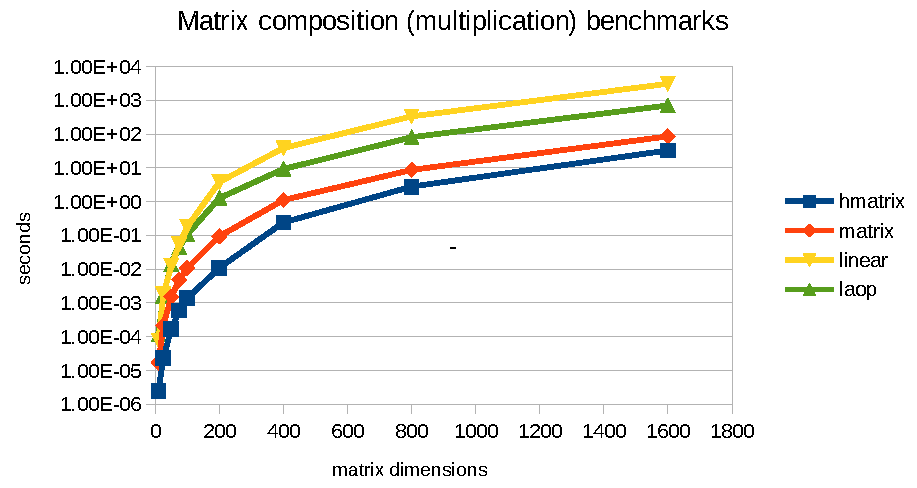
\includegraphics[width=\linewidth]{img/report1.pdf}
        \caption{Matrix composition benchmarks}
        \label{fig:bench}
    \end{figure}
    
    As can be seen in the plot of Figure \ref{fig:bench}, the \emph{hmatrix} and \emph{matrix} libraries are those that perform better. By observing their internal structure, one realises that they are a suitable representation for BLAS/LAPACK computations \citep{anderson1999lapack}, that is, they have been designed to efficiently exploit caches on modern cache-based architectures. A matrix in the \emph{linear} library is defined as \texttt{Vector cols (Vector rows Double)} and does not take into account cache lengths or sizes, so it behaves much worse than the previous ones. Our structure does not take into account any low-level optimisations either, being unable to compete with those that do. Nevertheless, the implementation is \emph{performant for a cache-oblivious approach} and behaves better (almost one order of magnitude better) than other types of simpler definitions.
        
        \subsection{Distribution matrix vs distribution list monad}
        
        The previous evaluation focused only on the performance of the matrix multiplication algorithm and compared with existing solutions to linear algebra however, in this section we will compare the use of matrices versus the use of lists as a representation of probability distributions, by comparing the performance of the \texttt{select} operator. Since both are exhaustive approaches to probabilistic programming, the comparisons will feature the applicative version of the \texttt{select} operator (where no computations are skipped) and see which solution performs best. Additionally, as we saw in section \ref{sec-eq-reason}, it is possible to have a more efficient version of the \texttt{select} operator, under the matrix representation, which we will call the selective version. This version is also going to be benchmarked and compared against its applicative alternative.
        
        The Figure and Listings below show the results output by the Criterion framework. The benchmarks were realized in the same settings as the previous one and, all matrices and lists were randomly generated.
        
            \begin{figure}[H]%[9]{r}{18em}
            \centering
             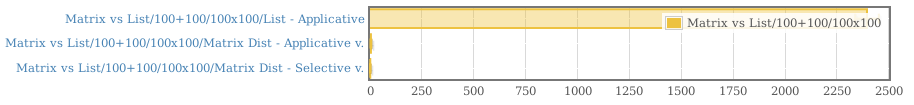
\includegraphics[width=\linewidth]{img/matrixVlist.png}
               \caption{Matrix vs List - \texttt{select} operator}
               \label{fig:bench2}
            \end{figure}
            
        \begin{lstlisting}[caption={Results}, captionpos=b]
benchmarking Matrix vs List/100+100/100x100/List - Applicative
time                 2.464 s    (2.411 s .. 2.515 s)
                     1.000 R^2   (1.000 R^2 .. 1.000 R^2)
mean                 2.395 s    (2.336 s .. 2.425 s)
std dev              56.98 ms   (2.896 ms .. 69.67 ms)
variance introduced by outliers: 19% (moderately inflated)

benchmarking Matrix vs List/100+100/100x100/Matrix Dist - Applicative v.
time                 2.607 ms   (2.007 ms .. 3.459 ms)
                     0.635 R^2   (0.538 R^2 .. 0.743 R^2)
mean                 4.451 ms   (3.848 ms .. 5.086 ms)
std dev              1.958 ms   (1.634 ms .. 2.399 ms)
variance introduced by outliers: 98% (severely inflated)

benchmarking Matrix vs List/100+100/100x100/Matrix Dist - Selective v.
time                 1.259 ms   (1.217 ms .. 1.329 ms)
                     0.962 R^2   (0.898 R^2 .. 0.995 R^2)
mean                 1.277 ms   (1.234 ms .. 1.383 ms)
std dev              210.0 micros   (124.3 micros .. 375.1 micros)
variance introduced by outliers: 87% (severely inflated)
        \end{lstlisting}{}
        
        The first entry corresponds to the distribution monad presented by \cite{erwig_kollmansberger_2006} and we can see that this solution is the one that performs worse. The applicative version of the \texttt{select} operator, in the matrix solution performs a lot better even though all computations are performed. The last entry refers to the selective version of the \texttt{select} operator and we can see that it outperforms the applicative version.
        
    \subsection{Sequential vs Concurrent Selective eDSL}
        In this section, the performance of each \gls{edsl} solution provided in the \ref{prob-edsl} and \ref{prob-conc} sections is evaluated. In order to do so, three probabilistic programs were used: one that threw two hypothetical $50000$ faced dice, returning both results; one that threw the same two dice but conditioned the result; and one similar to \texttt{diceThrow} in Listing \ref{lst:dicethrow} but using the same dice as the previous programs. As an example, see:
        
        \begin{lstlisting}[language=Haskell, caption={Programs used in evaluation}, captionpos=b]
bigDie :: Dist Int
bigDie = uniform [0 .. 50000]

pg1 :: Dist (Int, Int)
pg1 =
  let c1 = bigDie
      c2 = bigDie
   in (,) <$> c1 <*> c2

pg2 :: Dist (Maybe (Int, Int))
pg2 =
  let c1 = bigDie
      c2 = bigDie
      result = (,) <$> c1 <*> c2
   in condition (uncurry (>)) result

pg3 :: Dist Int
pg3 =
  condS
    (pure $ uncurry (==))
    ((\c (a, b) -> a + b + c) <$> die) -- Speculative dice throw
    (pure (\(a, _) -> a + a + a))
    ((,) <$> bigDie <*> bigDie) -- Parallel dice throw
        \end{lstlisting}{}
        
    Each benchmark consists of performing forward sampling $2000$ times. One thing to remember is that $4$ general benchmarks have been made. The first two interpret \gls{edsl} in a sequential fashion, directly to \texttt{IO}, and first to the concurrency monad, and then to \texttt{IO}. In the other two, the programs are written directly to the concurrency monad. These were the results:
    
    \begin{figure}[H]
        \centering
        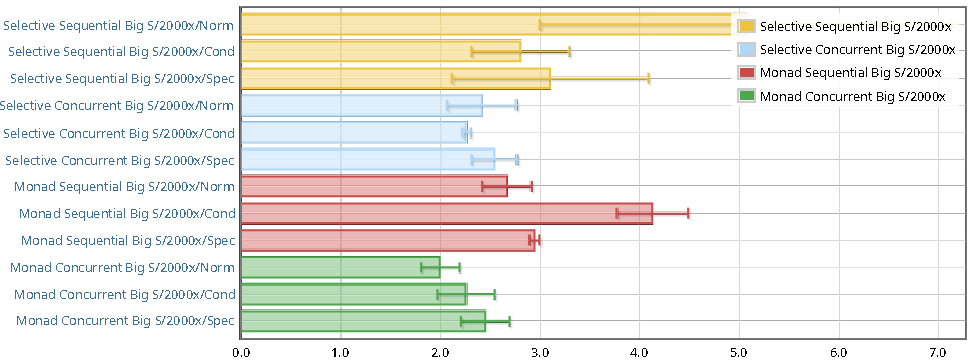
\includegraphics[width=\linewidth]{img/no-delay.pdf}
        \caption{Benchmarks results (No delay)}
        \label{fig:no-delay}
    \end{figure}
    
    As we can see from the graph, you can see that there are four distinct groups corresponding to the ones mentioned above. Absolute values are not that important, rather looking at them compared to each other will give us a much quicker and clearer interpretation of what's going on.
    
    The baseline results are the first three, and from a quick glance, we can see that the concurrent version is faster than the sequential one, but there are cases where the gains are not that high. This is due to the fact that sampling, even from a large random distribution such as \texttt{uniform 5000}, is very fast and thus there is not a large gap between sequential and concurrent versions.
    
    In order to unleash the full power of our solution, we decided to implement a small amount of delay (at least $100$ microseconds) between sample requests in order to simulate a large sample from a hypothetical big data source. The findings have been as follows:
    
    \begin{figure}[H]
        \centering
        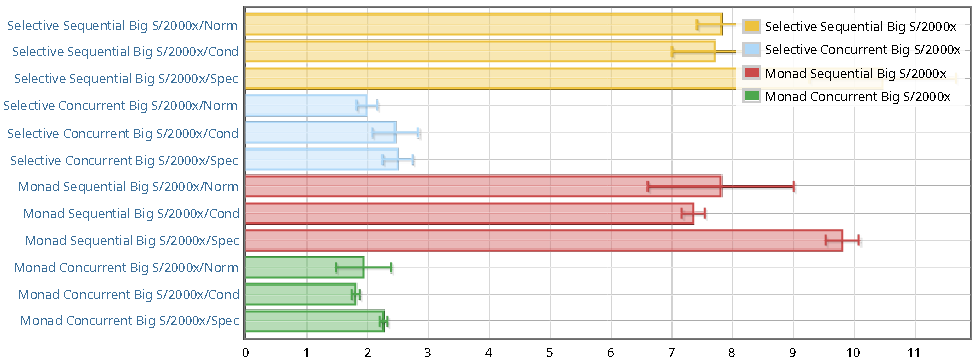
\includegraphics[width=\linewidth]{img/delay.pdf}
        \caption{Benchmarks results (delay)}
        \label{fig:delay}
    \end{figure}
    
    So, because of the delay that was implemented, the sequential versions are slower in this case, but the performance gains between the sequential and concurrent versions were larger and more evident than in the previous results.
        
	% CHAPTER - Conclusion/Future Work --------------
	\chapter{Conclusions and future work}\label{ch-conclusion}
	    In this chapter we’ll summarise the primary contributions of the dissertation and demonstrate that they defend the thesis. We'll also discuss some possible future work directions.
	
	    \section{Conclusions}
	        In this master thesis, we searched for a way to use \glspl{saf} in functional probabilistic programming, in particular to explore how this abstraction could be applied in a more efficient manner than the monadic \texttt{bind}. In order to do that, it was important to understand what these functors' probabilistic meaning was and what they could bring to the table. It is also important to consider what existing solutions and methods exist, and their drawbacks. We centered on the general theory of \gls{laop} when searching for answers to the probabilistic sense, and studied the structure of stochastic matrices, where we found that \glspl{saf} is capable of conditioning random variables and branching a program in two different ways. We realised that, through this prism, \glspl{saf} generalises the already known McCarthy conditional and, theoretically, allows for parallel execution of conditional probability calculations by means of the divide-and-conquer block-matrix algebra law. A programming library of typed inductive block-matrices has been implemented in Haskell to demonstrate how the findings of the research can be applied in practice, and a number of examples and benchmarks have been made available, demonstrating that the theoretical gains are indeed valid. However, the use of matrices in probabilistic programming has its drawbacks, namely in relation to programs where the sample space has an explosion of potential states. Sampling of the probability distributions should be done in these cases. However, existing solutions rely heavily on the use of monads that are inherently sequential, leaving behind any possibility of parallel sampling wherever possible. In order to solve this problem, a small probabilistic programming \gls{edsl} has been developed using the free \gls{saf} construction. Using this method, we push the end-user to use selective combinators wherever possible, so that the compiler can be sure to take advantage of the capabilities of this abstraction. The crucial insight that made it possible was to realise that the problem of sampling could be reduced to a concurrent external data access problem. Knowing this, it was possible to implement a solution close to the Haxl system and use it in our \gls{edsl}. The findings were positive compared to the previous sequential version. In view of this, it can be inferred that, due to the nature of \glspl{saf}, it was possible to use static analysis and speculative execution to write the \texttt{select} operator more efficiently than the monadic \texttt{bind}.
	        
	    \section{Future work}
	    
	     The work presented in this dissertation highlights the themes of composition, abstraction and structure, thes are relevant concepts in functional programming. The majority of features developed during this thesis are focused on important core aspects of static, purely functional languages. Monads, definitely the key driver of innovation, are difficult to express faithfully without a strong type system and functional purity, but as we have seen, these features have enabled us to have a great deal of reasoning power and have helped us to study novel abstractions in a different (probabilistic) context.
	    
	     One of the most important avenues for future work would also be to make the various pieces of software that have been developed during this research production-ready. Such projects necessarily have a proof-of-concept feeling about them; they are meant to explore new fields and opportunities. Specifically, quadtrees \citep{samet1984quadtree} and their savings with respect to repetitive cells (pixels) are brought to mind by the block-oriented matrix type from the typed matrix programming library. A better matrix definition for sparsity could be more useful for sparse matrices with large zero blocks.  The probabilistic programming \gls{edsl} can also be extended in order to support more distribution primitives and sampling algorithms. An interesting future direction is also to investigate improving the proposed solution in the light of the new found concurrency relationship, as well as studying parallelization strategies to improve performance. 
	     
	\bookmarksetup{startatroot} % Ends last part.
	\addtocontents{toc}{\bigskip} % Making the table of contents look good.
	%\cleardoublepage

	%- Bibliography (needs bibtex) -%
	\bibliography{dissertation}

	% Index of terms (needs  makeindex) -------------
	%\printindex
	
	
	% APPENDIX --------------------------------------
	\umappendix{Appendix}
	
	% Add appendix chapters
	\chapter{Type safe LAoP matrix wrapper library}\label{appendix-a}
	
    \begin{lstlisting}[language=Haskell, caption={Matrix.Internal},captionpos=b]
{-# LANGUAGE AllowAmbiguousTypes #-}
{-# LANGUAGE ConstraintKinds #-}
{-# LANGUAGE DataKinds #-}
{-# LANGUAGE FlexibleContexts #-}
{-# LANGUAGE FlexibleInstances #-}
{-# LANGUAGE GADTs #-}
{-# LANGUAGE GeneralizedNewtypeDeriving #-}
{-# LANGUAGE InstanceSigs #-}
{-# LANGUAGE KindSignatures #-}
{-# LANGUAGE MultiParamTypeClasses #-}
{-# LANGUAGE NoStarIsType #-}
{-# LANGUAGE ScopedTypeVariables #-}
{-# LANGUAGE StandaloneDeriving #-}
{-# LANGUAGE TypeApplications #-}
{-# LANGUAGE TypeOperators #-}
{-# LANGUAGE UndecidableInstances #-}
{-# OPTIONS_GHC -fplugin GHC.TypeLits.KnownNat.Solver #-}

module Matrix.Internal
  ( Matrix (..),
    NonZero,
    ValidDimensions,
    KnownDimensions,
    fromLists,
    toLists,
    toList,
    columns,
    rows,
    matrix,
    tr,
    row,
    col,
    fmapRows,
    fmapColumns,
    ident,
    zeros,
    ones,
    bang,
    diag,
    (|||),
    (===),
    i1,
    i2,
    p1,
    p2,
    (-|-),
    (><),
    kp1,
    kp2,
    khatri,
    selectM,
    comp,
    fromF,
  )
where

import Control.DeepSeq
import Data.Binary
import qualified Data.List as L
import Data.Proxy
import Foreign.Storable
import GHC.TypeLits
import qualified Numeric.LinearAlgebra as LA
import qualified Numeric.LinearAlgebra.Data as HM

-- | The 'Matrix' type is a type safe wrapper around the
-- 'Numeric.LinearAlgebra.Data.Matrix' data type.
newtype Matrix e (c :: Nat) (r :: Nat) = M {unMatrix :: HM.Matrix e}

deriving instance (LA.Container HM.Matrix e) => Eq (Matrix e c r)

deriving instance (LA.Container HM.Vector e, Fractional e, Fractional (HM.Vector e), Num (HM.Matrix e)) => Fractional (Matrix e c r)

deriving instance (Floating e, LA.Container HM.Vector e, Floating (HM.Vector e), Fractional (HM.Matrix e)) => Floating (Matrix e c r)

deriving instance (LA.Container HM.Matrix e, Num e, Num (HM.Vector e)) => Num (Matrix e c r)

deriving instance (Read e, LA.Element e) => Read (Matrix e c r)

deriving instance (Binary (HM.Vector e), LA.Element e) => Binary (Matrix e c r)

deriving instance (Storable e, NFData e) => NFData (Matrix e c r)

instance (Show e, LA.Element e) => Show (Matrix e c r) where
  show (M m) = show m

type NonZero (n :: Nat) = (CmpNat n 0 ~ 'GT)

type ValidDimensions (n :: Nat) (m :: Nat) = (NonZero n, NonZero m)

type KnownDimensions (n :: Nat) (m :: Nat) = (KnownNat n, KnownNat m)

-------------------------------------------------------------------------------
--    CONVERTER FUNCTIONS
-------------------------------------------------------------------------------

-- | Matrix converter function. It builds a matrix from
-- a list of lists @[[e]]@ (considered as rows).
fromLists :: forall e c r. (LA.Element e, KnownDimensions c r) => [[e]] -> Matrix e c r
fromLists [] = error "Wrong list dimensions"
fromLists l@(h : _) =
  let ccols = fromInteger $ natVal (Proxy :: Proxy c)
      rrows = fromInteger $ natVal (Proxy :: Proxy r)
      lrows = length l
      lcols = length h
   in if rrows /= lrows || ccols /= lcols
        then error "Wrong list dimensions"
        else M . HM.fromLists $ l

-- | Matrix converter function. It builds a list of lists from
-- a 'Matrix'.
--
-- Inverse of 'fromLists'.
toLists :: (LA.Element e) => Matrix e c r -> [[e]]
toLists = HM.toLists . unMatrix

-- | Matrix converter function. It builds a list of elements from
-- a 'Matrix'.
toList :: (LA.Element e) => Matrix e c r -> [e]
toList = concat . toLists

-- | Matrix converter function. It builds a matrix from a function.
fromF :: forall c r a b e. (Enum a, Enum b, Eq b, Num e, Ord e, LA.Element e, KnownNat c, KnownNat r) => (a -> b) -> Matrix e c r
fromF f =
  let ccols = fromInteger $ natVal (Proxy :: Proxy c)
      rrows = fromInteger $ natVal (Proxy :: Proxy r)
      elementsA = take ccols $ map toEnum [0 ..]
      elementsB = take rrows $ map toEnum [0 ..]
      combinations = (,) <$> elementsA <*> elementsB
      combAp = map snd . L.sort . map (\(a, b) -> if f a == b then ((fromEnum a, fromEnum b), 1) else ((fromEnum a, fromEnum b), 0)) $ combinations
      mList = buildList combAp rrows
   in tr $ fromLists mList
  where
    buildList [] _ = []
    buildList l r = take r l : buildList (drop r l) r

-------------------------------------------------------------------------------
--    DIMENSIONS FUNCTIONS
-------------------------------------------------------------------------------

-- | Obtain the number of columns of a matrix
columns :: forall e c r. KnownNat c => Matrix e c r -> Integer
columns _ = natVal (Proxy :: Proxy c)

-- | Obtain the number of rows of a matrix
rows :: forall e c r. KnownNat r => Matrix e c r -> Integer
rows _ = natVal (Proxy :: Proxy r)

fmapColumns :: forall b e a r. (Storable e, LA.Element e, KnownNat b) => Matrix e a r -> Matrix e b r
fmapColumns =
  let cols = fromInteger $ natVal (Proxy :: Proxy b)
   in M . HM.reshape cols . HM.fromList . toList

fmapRows :: forall b e a c. (Storable e, LA.Element e, KnownDimensions c b) => Matrix e c a -> Matrix e c b
fmapRows =
  let rows = fromInteger $ natVal (Proxy :: Proxy b)
   in tr . M . HM.reshape rows . HM.fromList . toList

-------------------------------------------------------------------------------
--    MISC FUNCTIONS
-------------------------------------------------------------------------------

-- | Create a matrix.
matrix :: forall e c r. (KnownDimensions c r, Storable e) => [e] -> Matrix e c r
matrix l =
  let m = (reshape @e @c) . HM.fromList $ l
      mcols = HM.cols (unMatrix m)
      mrows = HM.rows (unMatrix m)
      ccols = fromInteger $ natVal (Proxy :: Proxy c)
      rrows = fromInteger $ natVal (Proxy :: Proxy r)
   in if mcols /= ccols || mrows /= rrows
        then error "Wrong list dimensions"
        else m

-- | Matrix transpose
tr :: forall e c r. (LA.Element e, KnownDimensions c r) => Matrix e c r -> Matrix e r c
tr = fromLists . L.transpose . toLists

-- | Create a row vector matrix.
row :: (Storable e, LA.Element e, KnownNat c) => [e] -> Matrix e c 1
row = asRow . HM.fromList

-- | Create a column vector matrix.
col :: (Storable e) => [e] -> Matrix e 1 r
col = asColumn . HM.fromList

-- | Creates the identity matrix of given dimension.
ident :: forall e c. (Num e, LA.Element e, KnownNat c) => Matrix e c c
ident =
  let c = fromInteger $ natVal (Proxy :: Proxy c)
   in M . HM.ident $ c

-- | Zero Matrix polymorphic definition
zeros :: forall e c r. (KnownDimensions c r, Num e, LA.Container HM.Vector e) => Matrix e c r
zeros =
  let ccols = fromInteger $ natVal (Proxy :: Proxy c)
      rrows = fromInteger $ natVal (Proxy :: Proxy r)
   in M $ HM.konst 0 (rrows, ccols)

-- | One Matrix polymorphic definition
ones :: forall e c r. (KnownDimensions c r, Num e, LA.Container HM.Vector e) => Matrix e c r
ones =
  let ccols = fromInteger $ natVal (Proxy :: Proxy c)
      rrows = fromInteger $ natVal (Proxy :: Proxy r)
   in M $ HM.konst 1 (rrows, ccols)

-- | Bang Matrix polymorphic Matrix
bang :: forall e c . (KnownNat c, Num e, LA.Container HM.Vector e) => Matrix e c 1
bang =
  let ccols = fromInteger $ natVal (Proxy :: Proxy c)
   in M $ HM.konst 1 (1, ccols)

-- | Creates a square matrix with a given diagonal.
diag :: forall e c. (Num e, LA.Element e, KnownNat c) => [e] -> Matrix e c c
diag l =
  let c = fromInteger $ natVal (Proxy :: Proxy c)
      dims = length l
   in if c /= dims
        then error "Wrong list dimensions"
        else M . HM.diag . HM.fromList $ l

-------------------------------------------------------------------------------
--    BLOCK MATRIX FUNCTIONS (BIPRODUCT)
-------------------------------------------------------------------------------

-- | Matrix block algebra 'Junc' operator
(|||) :: (LA.Element e, ValidDimensions n m, NonZero p) => Matrix e m p -> Matrix e n p -> Matrix e (m + n) p
(|||) a b = M $ HM.fromBlocks [[unMatrix a, unMatrix b]]

infixl 3 |||

-- | Matrix block algebra 'Split' operator
(===) :: (LA.Element e, ValidDimensions n m, NonZero p) => Matrix e p m -> Matrix e p n -> Matrix e p (m + n)
(===) a b = M $ HM.fromBlocks [[unMatrix a], [unMatrix b]]

infixl 2 ===

-- | Matrix 'Junc' left injection matrix definition
i1 :: (Num e, ValidDimensions n m, KnownDimensions n m, LA.Element e, LA.Container HM.Vector e) => Matrix e m (m + n)
i1 = ident === zeros

-- | Matrix 'Junc' right injection matrix definition
i2 :: (Num e, ValidDimensions n m, KnownDimensions n m, LA.Element e, LA.Container HM.Vector e) => Matrix e n (m + n)
i2 = zeros === ident

-- | Matrix 'Split' left projection matrix definition
p1 :: (Num e, ValidDimensions n m, KnownDimensions n m, KnownNat (m + n), LA.Element e, LA.Container HM.Vector e) => Matrix e (m + n) m
p1 = tr i1

-- | Matrix 'Split' right projection matrix definition
p2 :: (Num e, ValidDimensions n m, KnownDimensions n m, KnownNat (m + n), LA.Element e, LA.Container HM.Vector e) => Matrix e (m + n) n
p2 = tr i2

-------------------------------------------------------------------------------
--    MATRIX BIPRODUCT FUNCTORS
-------------------------------------------------------------------------------

-- | Matrix coproduct bifunctor
(-|-) ::
  forall e n m j k.
  ( ValidDimensions n m,
    ValidDimensions k j,
    NonZero (k + j),
    LA.Element e,
    LA.Numeric e,
    KnownDimensions k j
  ) =>
  Matrix e n k ->
  Matrix e m j ->
  Matrix e (n + m) (k + j)
(-|-) a b = (i1 `comp` a) ||| (i2 `comp` b)

infixl 5 -|-

-- | Kronecker product of two matrices
(><) :: LA.Product e => Matrix e m p -> Matrix e n q -> Matrix e (m * n) (p * q)
(><) (M a) (M b) = M . LA.kronecker a $ b

infixl 4 ><

-------------------------------------------------------------------------------
--    MATRIX SELECTVIE EQUIVALENT FUNCTION
-------------------------------------------------------------------------------

selectM ::
  ( LA.Numeric e,
    Enum a,
    Enum b,
    Ord e,
    Eq b,
    KnownDimensions m1 m2,
    ValidDimensions m1 m2
  ) =>
  Matrix e n (m1 + m2) -> (a -> b) -> Matrix e n m2
selectM m y = (fromF y ||| ident) `comp` m

-------------------------------------------------------------------------------
--    MATRIX COMPOSITION, KHATRI RAO FUNCTIONS
-------------------------------------------------------------------------------

-- | Matrix - Matrix multiplication aka Matrix composition
comp :: LA.Numeric e => Matrix e p m -> Matrix e n p -> Matrix e n m
comp (M a) (M b) = M . (LA.<>) a $ b

-- | Khatri Rao product left projection (inductive definition)
class KhatriP1 e (m :: Nat) (k :: Nat) where
  kp1 :: Matrix e (m * k) m

instance
  {-# OVERLAPPING #-}
  ( KnownNat k,
    Num e,
    LA.Numeric e,
    LA.Container HM.Vector e
  ) =>
  KhatriP1 e 1 k
  where
  kp1 = ones @e @k @1

instance
  {-# OVERLAPPABLE #-}
  ( ValidDimensions m k,
    KnownNat k,
    KnownNat ((m - 1) * k),
    KnownNat (m - 1),
    Num e,
    LA.Numeric e,
    LA.Container HM.Vector e,
    (1 + (m - 1)) ~ m,
    (k + ((m - 1) * k)) ~ (m * k),
    NonZero ((m - 1) * k),
    NonZero (m - 1),
    KhatriP1 e (m - 1) k
  ) =>
  KhatriP1 e m k
  where
  kp1 = ones @e @k @1 -|- kp1 @e @(m - 1) @k

-- | Khatri Rao product right projection (inductive definition)
class KhatriP2 e (k :: Nat) (m :: Nat) where
  kp2 :: Matrix e (m * k) k

instance
  {-# OVERLAPPING #-}
  ( Num e,
    LA.Element e,
    KnownNat k
  ) =>
  KhatriP2 e k 1
  where
  kp2 = ident @e @k

instance
  {-# OVERLAPPABLE #-}
  ( (k + ((m - 1) * k)) ~ (m * k),
    ValidDimensions m k,
    NonZero ((m - 1) * k),
    LA.Element e,
    Num e,
    KnownNat k,
    KhatriP2 e k (m - 1)
  ) =>
  KhatriP2 e k m
  where
  kp2 = ident @e @k ||| kp2 @e @k @(m - 1)

-- | Khatri Rao product of two matrices (Pairing)
khatri ::
  forall e m p q.
  ( KnownDimensions p (p * q),
    KnownNat q,
    Num e,
    Num (HM.Vector e),
    LA.Numeric e,
    LA.Container HM.Vector e,
    KhatriP1 e p q,
    KhatriP2 e q p
  ) =>
  Matrix e m p ->
  Matrix e m q ->
  Matrix e m (p * q)
khatri a b = (tr (kp1 @e @p @q) `comp` a) * (tr (kp2 @e @q @p) `comp` b)

-------------------------------------------------------------------------------
--    AUXILIARY FUNCTIONS
-------------------------------------------------------------------------------

-- | Creates a matrix from a vector by grouping the elements in rows
-- with the desired number of columns.
reshape :: forall e c r. (Storable e, KnownNat c) => HM.Vector e -> Matrix e c r
reshape v =
  let cols = fromInteger $ natVal (Proxy :: Proxy c)
   in M $ HM.reshape cols v

-- | Creates a 1-column matrix from a vector.
asColumn :: forall e r. (Storable e) => HM.Vector e -> Matrix e 1 r
asColumn = reshape @e @1

-- | Creates a 1-vector matrix from a vector.
asRow :: (Storable e, LA.Element e, KnownNat c) => HM.Vector e -> Matrix e c 1
asRow = tr . asColumn
    \end{lstlisting}
    
	\chapter{Type safe LAoP inductive matrix definition library}\label{appendix-b}
	
    \begin{lstlisting}[language=Haskell, caption={Matrix.Internal},captionpos=b]
{-# LANGUAGE AllowAmbiguousTypes #-}
{-# LANGUAGE DataKinds #-}
{-# LANGUAGE FlexibleContexts #-}
{-# LANGUAGE FlexibleInstances #-}
{-# LANGUAGE GADTs #-}
{-# LANGUAGE InstanceSigs #-}
{-# LANGUAGE MultiParamTypeClasses #-}
{-# LANGUAGE NoStarIsType #-}
{-# LANGUAGE ScopedTypeVariables #-}
{-# LANGUAGE StandaloneDeriving #-}
{-# LANGUAGE TypeApplications #-}
{-# LANGUAGE TypeFamilies #-}
{-# LANGUAGE TypeOperators #-}
{-# LANGUAGE UndecidableInstances #-}

-----------------------------------------------------------------------------
-- |
-- Module     : Matrix.Internal
-- Copyright  : (c) Armando Santos 2019-2020
-- Maintainer : armandoifsantos@gmail.com
-- Stability  : experimental
--
-- The LAoP discipline generalises relations and functions treating them as
-- Boolean matrices and in turn consider these as arrows.
--
-- __LAoP__ is a library for algebraic (inductive) construction and manipulation of matrices
-- in Haskell. See <https://github.com/bolt12/master-thesis my Msc Thesis> for the
-- motivation behind the library, the underlying theory, and implementation details.
--
-- This module offers many of the combinators mentioned in the work of
-- Macedo (2012) and Oliveira (2012). 
--
-- This is an Internal module and it is no supposed to be imported.
--
-----------------------------------------------------------------------------

module Matrix.Internal
  ( -- | This definition makes use of the fact that 'Void' is
    -- isomorphic to 0 and '()' to 1 and captures matrix
    -- dimensions as stacks of 'Either's.
    --
    -- There exists two type families that make it easier to write
    -- matrix dimensions: 'FromNat' and 'Count'. This approach
    -- leads to a very straightforward implementation 
    -- of LAoP combinators. 

    -- * Type safe matrix representation
    Matrix (..),

    -- * Primitives
    empty,
    one,
    junc,
    split,

    -- * Auxiliary type families
    FromNat,
    Count,
    Normalize,

    -- * Matrix construction and conversion
    FromLists,
    fromLists,
    toLists,
    toList,
    matrixBuilder,
    row,
    col,
    zeros,
    ones,
    bang,
    constant,

    -- * Misc
    -- ** Get dimensions
    columns,
    rows,

    -- ** Matrix Transposition
    tr,

    -- ** Selective operator
    select, 

    -- ** McCarthy's Conditional
    cond,

    -- ** Matrix "abiding"
    abideJS,
    abideSJ,

    -- * Biproduct approach
    -- ** Split
    (===),
    -- *** Projections
    p1,
    p2,
    -- ** Junc
    (|||),
    -- *** Injections
    i1,
    i2,
    -- ** Bifunctors
    (-|-),
    (><),

    -- ** Applicative matrix combinators

    -- | Note that given the restrictions imposed it is not possible to
    -- implement the standard type classes present in standard Haskell.
    -- *** Matrix pairing projections
    kp1,
    kp2,

    -- *** Matrix pairing
    khatri,

    -- * Matrix composition and lifting

    -- ** Arrow matrix combinators

    -- | Note that given the restrictions imposed it is not possible to
    -- implement the standard type classes present in standard Haskell.
    identity,
    comp,
    fromF,
    fromF',

    -- * Matrix printing
    pretty,
    prettyPrint
  )
    where

import Utils
import Data.Bool
import Data.Kind
import Data.List
import Data.Proxy
import Data.Void
import GHC.TypeLits
import Data.Type.Equality
import GHC.Generics
import Control.DeepSeq
import Control.Category
import Prelude hiding ((.))

-- | LAoP (Linear Algebra of Programming) Inductive Matrix definition.
data Matrix e cols rows where
  Empty :: Matrix e Void Void
  One :: e -> Matrix e () ()
  Junc :: Matrix e a rows -> Matrix e b rows -> Matrix e (Either a b) rows
  Split :: Matrix e cols a -> Matrix e cols b -> Matrix e cols (Either a b)

deriving instance (Show e) => Show (Matrix e cols rows)

-- | Type family that computes the cardinality of a given type dimension.
--
--   It can also count the cardinality of custom types that implement the
-- 'Generic' instance.
type family Count (d :: Type) :: Nat where
  Count (Natural n m) = (m - n) + 1
  Count (Either a b) = (+) (Count a) (Count b)
  Count (a, b) = (*) (Count a) (Count b)
  Count (a -> b) = (^) (Count b) (Count a)
  -- Generics
  Count (M1 _ _ f p) = Count (f p)
  Count (K1 _ _ _) = 1
  Count (V1 _) = 0
  Count (U1 _) = 1
  Count ((:*:) a b p) = Count (a p) * Count (b p)
  Count ((:+:) a b p) = Count (a p) + Count (b p)
  Count d = Count (Rep d R)

-- | Type family that computes of a given type dimension from a given natural
--
--   Thanks to Li-Yao Xia this type family is super fast.
type family FromNat (n :: Nat) :: Type where
  FromNat 0 = Void
  FromNat 1 = ()
  FromNat n = FromNat' (Mod n 2 == 0) (FromNat (Div n 2))

type family FromNat' (b :: Bool) (m :: Type) :: Type where
  FromNat' 'True m = Either m m
  FromNat' 'False m = Either () (Either m m)

-- | Type family that normalizes the representation of a given data
-- structure
type family Normalize (d :: Type) :: Type where
  Normalize d = FromNat (Count d)

-- | It is not possible to implement the 'id' function so it is
-- implementation is 'undefined'. However 'comp' can be and this partial
-- class implementation exists just to make the code more readable.
--
-- Please use 'identity' instead.
instance (Num e) => Category (Matrix e) where
    id = undefined
    (.) = comp

instance NFData e => NFData (Matrix e cols rows) where
    rnf Empty = ()
    rnf (One e) = rnf e
    rnf (Junc a b) = rnf a `seq` rnf b
    rnf (Split a b) = rnf a `seq` rnf b

instance Eq e => Eq (Matrix e cols rows) where
  Empty == Empty                = True
  (One a) == (One b)            = a == b
  (Junc a b) == (Junc c d)      = a == c && b == d
  (Split a b) == (Split c d)    = a == c && b == d
  x@(Split a b) == y@(Junc c d) = x == abideJS y
  x@(Junc a b) == y@(Split c d) = abideJS x == y

instance Num e => Num (Matrix e cols rows) where

  Empty + Empty                = Empty
  (One a) + (One b)            = One (a + b)
  (Junc a b) + (Junc c d)      = Junc (a + c) (b + d)
  (Split a b) + (Split c d)    = Split (a + c) (b + d)
  x@(Split a b) + y@(Junc c d) = x + abideJS y
  x@(Junc a b) + y@(Split c d) = abideJS x + y

  Empty - Empty             = Empty
  (One a) - (One b)         = One (a - b)
  (Junc a b) - (Junc c d)   = Junc (a - c) (b - d)
  (Split a b) - (Split c d) = Split (a - c) (b - d)
  x@(Split a b) - y@(Junc c d) = x - abideJS y
  x@(Junc a b) - y@(Split c d) = abideJS x - y

  Empty * Empty             = Empty
  (One a) * (One b)         = One (a * b)
  (Junc a b) * (Junc c d)   = Junc (a * c) (b * d)
  (Split a b) * (Split c d) = Split (a * c) (b * d)
  x@(Split a b) * y@(Junc c d) = x * abideJS y
  x@(Junc a b) * y@(Split c d) = abideJS x * y

  abs Empty       = Empty
  abs (One a)     = One (abs a)
  abs (Junc a b)  = Junc (abs a) (abs b)
  abs (Split a b) = Split (abs a) (abs b)

  signum Empty       = Empty
  signum (One a)     = One (signum a)
  signum (Junc a b)  = Junc (signum a) (signum b)
  signum (Split a b) = Split (signum a) (signum b)

-- Primitives

-- | Empty matrix constructor
empty :: Matrix e Void Void
empty = Empty

-- | Unit matrix constructor
one :: e -> Matrix e () ()
one = One

-- | Matrix 'Junc' constructor
junc :: Matrix e a rows -> Matrix e b rows -> Matrix e (Either a b) rows
junc = Junc

infixl 3 |||

-- | Matrix 'Junc' constructor
(|||) :: Matrix e a rows -> Matrix e b rows -> Matrix e (Either a b) rows
(|||) = Junc

-- | Matrix 'Split' constructor
split :: Matrix e cols a -> Matrix e cols b -> Matrix e cols (Either a b)
split = Split

infixl 2 ===

-- | Matrix 'Split' constructor
(===) :: Matrix e cols a -> Matrix e cols b -> Matrix e cols (Either a b)
(===) = Split

-- Construction

-- | Type class for defining the 'fromList' conversion function.
--
--   Given that it is not possible to branch on types at the term level type
-- classes are needed bery much like an inductive definition but on types.
class FromLists e cols rows where
  -- | Build a matrix out of a list of list of elements. Throws a runtime
  -- error if the dimensions do not match.
  fromLists :: [[e]] -> Matrix e cols rows

instance FromLists e Void Void where
  fromLists [] = Empty
  fromLists _  = error "Wrong dimensions"

instance {-# OVERLAPPING #-} FromLists e () () where
  fromLists [[e]] = One e
  fromLists _     = error "Wrong dimensions"

instance {-# OVERLAPPING #-} (FromLists e cols ()) => FromLists e (Either () cols) () where
  fromLists [h : t] = Junc (One h) (fromLists [t])
  fromLists _       = error "Wrong dimensions"

instance {-# OVERLAPPABLE #-} (FromLists e a (), FromLists e b (), KnownNat (Count a)) => FromLists e (Either a b) () where
  fromLists [l] = 
      let rowsA = fromInteger (natVal (Proxy :: Proxy (Count a)))
       in Junc (fromLists [take rowsA l]) (fromLists [drop rowsA l])
  fromLists _       = error "Wrong dimensions"

instance {-# OVERLAPPING #-} (FromLists e () rows) => FromLists e () (Either () rows) where
  fromLists ([h] : t) = Split (One h) (fromLists t)
  fromLists _         = error "Wrong dimensions"

instance {-# OVERLAPPABLE #-} (FromLists e () a, FromLists e () b, KnownNat (Count a)) => FromLists e () (Either a b) where
  fromLists l@([h] : t) = 
      let rowsA = fromInteger (natVal (Proxy :: Proxy (Count a)))
       in Split (fromLists (take rowsA l)) (fromLists (drop rowsA l))
  fromLists _         = error "Wrong dimensions"

instance {-# OVERLAPPABLE #-} (FromLists e (Either a b) c, FromLists e (Either a b) d, KnownNat (Count c)) => FromLists e (Either a b) (Either c d) where
  fromLists l@(h : t) =
    let lh        = length h
        rowsC     = fromInteger (natVal (Proxy :: Proxy (Count c)))
        condition = all (== lh) (map length t)
     in if lh > 0 && condition
          then Split (fromLists (take rowsC l)) (fromLists (drop rowsC l))
          else error "Not all rows have the same length"

-- | Matrix builder function. Constructs a matrix provided with
-- a construction function.
matrixBuilder ::
  forall e cols rows.
  ( FromLists e cols rows,
    KnownNat (Count cols),
    KnownNat (Count rows)
  ) =>
  ((Int, Int) -> e) ->
  Matrix e cols rows
matrixBuilder f =
  let c         = fromInteger $ natVal (Proxy :: Proxy (Count cols))
      r         = fromInteger $ natVal (Proxy :: Proxy (Count rows))
      positions = [(a, b) | a <- [0 .. (r - 1)], b <- [0 .. (c - 1)]]
   in fromLists . map (map f) . groupBy (\(x, _) (w, _) -> x == w) $ positions

-- | Constructs a column vector matrix
col :: (FromLists e () rows) => [e] -> Matrix e () rows
col = fromLists . map (: [])

-- | Constructs a row vector matrix
row :: (FromLists e cols ()) => [e] -> Matrix e cols ()
row = fromLists . (: [])

-- | Lifts functions to matrices with arbitrary dimensions.
--
--   NOTE: Be careful to not ask for a matrix bigger than the cardinality of
-- types @a@ or @b@ allows.
fromF ::
  forall a b cols rows e.
  ( Bounded a,
    Bounded b,
    Enum a,
    Enum b,
    Eq b,
    Num e,
    Ord e,
    KnownNat (Count cols),
    KnownNat (Count rows),
    FromLists e rows cols
  ) =>
  (a -> b) ->
  Matrix e cols rows
fromF f =
  let minA         = minBound @a
      maxA         = maxBound @a
      minB         = minBound @b
      maxB         = maxBound @b
      ccols        = fromInteger $ natVal (Proxy :: Proxy (Count cols))
      rrows        = fromInteger $ natVal (Proxy :: Proxy (Count rows))
      elementsA    = take ccols [minA .. maxA]
      elementsB    = take rrows [minB .. maxB]
      combinations = (,) <$> elementsA <*> elementsB
      combAp       = map snd . sort . map (\(a, b) -> if f a == b 
                                                         then ((fromEnum a, fromEnum b), 1) 
                                                         else ((fromEnum a, fromEnum b), 0)) $ combinations
      mList        = buildList combAp rrows
   in tr $ fromLists mList
  where
    buildList [] _ = []
    buildList l r  = take r l : buildList (drop r l) r

-- | Lifts functions to matrices with dimensions matching @a@ and @b@
-- cardinality's.
fromF' ::
  forall a b e.
  ( Bounded a,
    Bounded b,
    Enum a,
    Enum b,
    Eq b,
    Num e,
    Ord e,
    KnownNat (Count (Normalize a)),
    KnownNat (Count (Normalize b)),
    FromLists e (Normalize b) (Normalize a)
  ) =>
  (a -> b) ->
  Matrix e (Normalize a) (Normalize b)
fromF' f =
  let minA         = minBound @a
      maxA         = maxBound @a
      minB         = minBound @b
      maxB         = maxBound @b
      ccols        = fromInteger $ natVal (Proxy :: Proxy (Count (Normalize a)))
      rrows        = fromInteger $ natVal (Proxy :: Proxy (Count (Normalize b)))
      elementsA    = take ccols [minA .. maxA]
      elementsB    = take rrows [minB .. maxB]
      combinations = (,) <$> elementsA <*> elementsB
      combAp       = map snd . sort . map (\(a, b) -> if f a == b 
                                                         then ((fromEnum a, fromEnum b), 1) 
                                                         else ((fromEnum a, fromEnum b), 0)) $ combinations
      mList        = buildList combAp rrows
   in tr $ fromLists mList
  where
    buildList [] _ = []
    buildList l r  = take r l : buildList (drop r l) r

-- Conversion

-- | Converts a matrix to a list of lists of elements.
toLists :: Matrix e cols rows -> [[e]]
toLists Empty       = []
toLists (One e)     = [[e]]
toLists (Split l r) = toLists l ++ toLists r
toLists (Junc l r)  = zipWith (++) (toLists l) (toLists r)

-- | Converts a matrix to a list of elements.
toList :: Matrix e cols rows -> [e]
toList = concat . toLists

-- Zeros Matrix

-- | The zero matrix. A matrix wholly filled with zeros.
zeros :: (Num e, FromLists e cols rows, KnownNat (Count cols), KnownNat (Count rows)) => Matrix e cols rows
zeros = matrixBuilder (const 0)

-- Ones Matrix

-- | The ones matrix. A matrix wholly filled with ones.
--
--   Also known as T (Top) matrix.
ones :: (Num e, FromLists e cols rows, KnownNat (Count cols), KnownNat (Count rows)) => Matrix e cols rows
ones = matrixBuilder (const 1)

-- Const Matrix

-- | The constant matrix constructor. A matrix wholly filled with a given
-- value.
constant :: (Num e, FromLists e cols rows, KnownNat (Count cols), KnownNat (Count rows)) => e -> Matrix e cols rows
constant e = matrixBuilder (const e)

-- Bang Matrix

-- | The T (Top) row vector matrix.
bang :: forall e cols. (Num e, Enum e, FromLists e cols (), KnownNat (Count cols)) => Matrix e cols ()
bang =
  let c = fromInteger $ natVal (Proxy :: Proxy (Count cols))
   in fromLists [take c [1, 1 ..]]

-- Identity Matrix

-- | Identity matrix.
identity :: (Num e, FromLists e cols cols, KnownNat (Count cols)) => Matrix e cols cols
identity = matrixBuilder (bool 0 1 . uncurry (==))

-- Matrix composition (MMM)

-- | Matrix composition. Equivalent to matrix-matrix multiplication.
--
--   This definition takes advantage of divide-and-conquer and fusion laws
-- from LAoP.
comp :: (Num e) => Matrix e cr rows -> Matrix e cols cr -> Matrix e cols rows
comp Empty Empty            = Empty
comp (One a) (One b)        = One (a * b)
comp (Junc a b) (Split c d) = comp a c + comp b d         -- Divide-and-conquer law
comp (Split a b) c          = Split (comp a c) (comp b c) -- Split fusion law
comp c (Junc a b)           = Junc (comp c a) (comp c b)  -- Junc fusion law

-- Projections

-- | Biproduct first component projection
p1 :: forall e m n. (Num e, KnownNat (Count n), KnownNat (Count m), FromLists e n m, FromLists e m m) => Matrix e (Either m n) m
p1 =
  let iden = identity :: Matrix e m m
      zero = zeros :: Matrix e n m
   in junc iden zero

-- | Biproduct second component projection
p2 :: forall e m n. (Num e, KnownNat (Count n), KnownNat (Count m), FromLists e m n, FromLists e n n) => Matrix e (Either m n) n
p2 =
  let iden = identity :: Matrix e n n
      zero = zeros :: Matrix e m n
   in junc zero iden

-- Injections

-- | Biproduct first component injection
i1 :: (Num e, KnownNat (Count n), KnownNat (Count m), FromLists e n m, FromLists e m m) => Matrix e m (Either m n)
i1 = tr p1

-- | Biproduct second component injection
i2 :: (Num e, KnownNat (Count n), KnownNat (Count m), FromLists e m n, FromLists e n n) => Matrix e n (Either m n)
i2 = tr p2

-- Dimensions

-- | Obtain the number of rows.
--
--   NOTE: The 'KnownNat' constaint is needed in order to obtain the
-- dimensions in constant time.
--
-- TODO: A 'rows' function that does not need the 'KnownNat' constraint in
-- exchange for performance.
rows :: forall e cols rows. (KnownNat (Count rows)) => Matrix e cols rows -> Int
rows _ = fromInteger $ natVal (Proxy :: Proxy (Count rows))

-- | Obtain the number of columns.
-- 
--   NOTE: The 'KnownNat' constaint is needed in order to obtain the
-- dimensions in constant time.
--
-- TODO: A 'columns' function that does not need the 'KnownNat' constraint in
-- exchange for performance.
columns :: forall e cols rows. (KnownNat (Count cols)) => Matrix e cols rows -> Int
columns _ = fromInteger $ natVal (Proxy :: Proxy (Count cols))

-- Coproduct Bifunctor

infixl 5 -|-

-- | Matrix coproduct functor also known as matrix direct sum.
(-|-) ::
  forall e n k m j.
  ( Num e,
    KnownNat (Count j),
    KnownNat (Count k),
    FromLists e k k,
    FromLists e j k,
    FromLists e k j,
    FromLists e j j
  ) =>
  Matrix e n k ->
  Matrix e m j ->
  Matrix e (Either n m) (Either k j)
(-|-) a b = Junc (i1 . a) (i2 . b)

-- Khatri Rao Product and projections

-- | Khatri Rao product first component projection matrix.
kp1 :: 
  forall e m k .
  ( Num e,
    KnownNat (Count k),
    FromLists e (FromNat (Count m * Count k)) m,
    KnownNat (Count m),
    KnownNat (Count (Normalize (m, k)))
  ) => Matrix e (Normalize (m, k)) m
kp1 = matrixBuilder f
  where
    offset = fromInteger (natVal (Proxy :: Proxy (Count k)))
    f (x, y)
      | y >= (x * offset) && y <= (x * offset + offset - 1) = 1
      | otherwise = 0

-- | Khatri Rao product second component projection matrix.
kp2 :: 
    forall e m k .
    ( Num e,
      KnownNat (Count k),
      FromLists e (FromNat (Count m * Count k)) k,
      KnownNat (Count m),
      KnownNat (Count (Normalize (m, k)))
    ) => Matrix e (Normalize (m, k)) k
kp2 = matrixBuilder f
  where
    offset = fromInteger (natVal (Proxy :: Proxy (Count k)))
    f (x, y)
      | x == y || mod (y - x) offset == 0 = 1
      | otherwise                         = 0

-- | Khatri Rao Matrix product also known as matrix pairing.
--
--   NOTE: That this is not a true categorical product, see for instance:
-- 
-- @
--                | kp1 . khatri a b == a 
-- khatri a b ==> |
--                | kp2 . khatri a b == b
-- @
--
-- __Emphasis__ on the implication symbol.
khatri :: 
       forall e cols a b. 
       ( Num e,
         KnownNat (Count a),
         KnownNat (Count b),
         KnownNat (Count (Normalize (a, b))),
         FromLists e (Normalize (a, b)) a,
         FromLists e (Normalize (a, b)) b
       ) => Matrix e cols a -> Matrix e cols b -> Matrix e cols (Normalize (a, b))
khatri a b =
  let kp1' = kp1 @e @a @b
      kp2' = kp2 @e @a @b
   in (tr kp1') . a * (tr kp2') . b

-- Product Bifunctor (Kronecker)

infixl 4 ><

-- | Matrix product functor also known as kronecker product
(><) :: 
     forall e m p n q. 
     ( Num e,
       KnownNat (Count m),
       KnownNat (Count n),
       KnownNat (Count p),
       KnownNat (Count q),
       KnownNat (Count (Normalize (m, n))),
       FromLists e (Normalize (m, n)) m,
       FromLists e (Normalize (m, n)) n,
       KnownNat (Count (Normalize (p, q))),
       FromLists e (Normalize (p, q)) p,
       FromLists e (Normalize (p, q)) q
     ) 
     => Matrix e m p -> Matrix e n q -> Matrix e (Normalize (m, n)) (Normalize (p, q))
(><) a b =
  let kp1' = kp1 @e @m @n
      kp2' = kp2 @e @m @n
   in khatri (a . kp1') (b . kp2')

-- Matrix abide Junc Split

-- | Matrix "abiding" followin the 'Junc'-'Split' abide law.
-- 
-- Law:
--
-- @
-- 'Junc' ('Split' a c) ('Split' b d) == 'Split' ('Junc' a b) ('Junc' c d)
-- @
abideJS :: Matrix e cols rows -> Matrix e cols rows
abideJS (Junc (Split a c) (Split b d)) = Split (Junc (abideJS a) (abideJS b)) (Junc (abideJS c) (abideJS d)) -- Junc-Split abide law
abideJS Empty                          = Empty
abideJS (One e)                        = One e
abideJS (Junc a b)                     = Junc (abideJS a) (abideJS b)
abideJS (Split a b)                    = Split (abideJS a) (abideJS b)

-- Matrix abide Split Junc

-- | Matrix "abiding" followin the 'Split'-'Junc' abide law.
-- 
-- @
-- 'Split' ('Junc' a b) ('Junc' c d) == 'Junc' ('Split' a c) ('Split' b d)
-- @
abideSJ :: Matrix e cols rows -> Matrix e cols rows
abideSJ (Split (Junc a b) (Junc c d)) = Junc (Split (abideSJ a) (abideSJ c)) (Split (abideSJ b) (abideSJ d)) -- Split-Junc abide law
abideSJ Empty                         = Empty
abideSJ (One e)                       = One e
abideSJ (Junc a b)                    = Junc (abideSJ a) (abideSJ b)
abideSJ (Split a b)                   = Split (abideSJ a) (abideSJ b)

-- Matrix transposition

-- | Matrix transposition.
tr :: Matrix e cols rows -> Matrix e rows cols
tr Empty       = Empty
tr (One e)     = One e
tr (Junc a b)  = Split (tr a) (tr b)
tr (Split a b) = Junc (tr a) (tr b)

-- Selective 'select' operator

-- | Selective functors 'select' operator equivalent inspired by the
-- ArrowMonad solution presented in the paper.
select :: 
       ( Bounded a,
         Bounded b,
         Enum a,
         Enum b,
         Num e,
         Ord e,
         Eq b,
         KnownNat (Count (Normalize a)),
         KnownNat (Count (Normalize b)),
         KnownNat (Count cols),
         FromLists e (Normalize b) (Normalize a),
         FromLists e (Normalize b) (Normalize b)
       ) => Matrix e cols (Either (Normalize a) (Normalize b)) -> (a -> b) -> Matrix e cols (Normalize b)
select m y = 
    let f = fromF y
     in junc f identity . m

-- McCarthy's Conditional

-- | McCarthy's Conditional expresses probabilistic choice.
cond ::
     ( cols ~ FromNat (Count cols),
       KnownNat (Count cols),
       FromLists e () cols,
       FromLists e cols (),
       FromLists e cols cols,
       Bounded a,
       Enum a,
       Num e,
       Ord e
     )
     =>
     (a -> Bool) -> Matrix e cols rows -> Matrix e cols rows -> Matrix e cols rows
cond p f g = junc f g . grd p

grd :: 
    ( q ~ FromNat (Count q),
      KnownNat (Count q),
      FromLists e () q,
      FromLists e q (),
      FromLists e q q,
      Bounded a,
      Enum a,
      Num e,
      Ord e
    )
    =>
    (a -> Bool) -> Matrix e q (Either q q)
grd f = split (corr f) (corr (not . f))

corr :: 
    forall e a q . 
    ( q ~ FromNat (Count q),
      KnownNat (Count q),
      FromLists e () q,
      FromLists e q (),
      FromLists e q q,
      Bounded a,
      Enum a,
      Num e,
      Ord e
    ) 
     => (a -> Bool) -> Matrix e q q
corr p = let f = fromF p :: Matrix e q ()
          in khatri f (identity :: Matrix e q q)

-- Pretty print

prettyAux :: Show e => [[e]] -> [[e]] -> String
prettyAux [] _     = ""
prettyAux [[e]] m   = "| " ++ fill (show e) ++ " |\n"
  where
   v  = fmap show m
   widest = maximum $ fmap length v
   fill str = replicate (widest - length str - 2) ' ' ++ str
prettyAux [h] m     = "| " ++ fill (unwords $ map show h) ++ " |\n"
  where
   v  = fmap show m
   widest = maximum $ fmap length v
   fill str = replicate (widest - length str - 2) ' ' ++ str
prettyAux (h : t) l = "| " ++ fill (unwords $ map show h) ++ " |\n" ++ 
                      prettyAux t l
  where
   v  = fmap show l
   widest = maximum $ fmap length v
   fill str = replicate (widest - length str - 2) ' ' ++ str

-- | Matrix pretty printer
pretty :: (KnownNat (Count cols), Show e) => Matrix e cols rows -> String
pretty m = "+ " ++ unwords (replicate (columns m) blank) ++ " +\n" ++ 
            prettyAux (toLists m) (toLists m) ++
            "+ " ++ unwords (replicate (columns m) blank) ++ " +"
  where
   v  = fmap show (toList m)
   widest = maximum $ fmap length v
   fill str = replicate (widest - length str) ' ' ++ str
   blank = fill ""

-- | Matrix pretty printer
prettyPrint :: (KnownNat (Count cols), Show e) => Matrix e cols rows -> IO ()
prettyPrint = putStrLn . pretty
    \end{lstlisting}
    
	\chapter{Selective probabilistic programming library}\label{appendix-c}
	
    \begin{lstlisting}[language=Haskell, caption={SelectiveProb.hs},captionpos=b]
{- |
Copyright: (c) 2020 Armando Santos
SPDX-License-Identifier: MIT
Maintainer: Armando Santos <armandoifsantos@gmail.com>

See README for more info
-}

{-# LANGUAGE DeriveFunctor #-}
{-# LANGUAGE DeriveAnyClass #-}
{-# LANGUAGE DeriveGeneric #-}
{-# LANGUAGE GADTs #-}
{-# LANGUAGE RankNTypes #-}

module SelectiveProb where

import Control.Concurrent
import Control.Concurrent.Async
import Control.DeepSeq
import Control.Selective
import Control.Selective.Free
import Data.Bifunctor
import Data.Bool
import Data.Foldable (toList)
import Data.Functor.Identity
import Data.IORef
import Data.List (group, maximumBy, sort)
import Data.Ord
import qualified Data.Vector as V
import Data.Sequence (Seq, singleton)
import GHC.Generics
import qualified System.Random.MWC.Probability as MWCP

data BlockedRequest = forall a. BlockedRequest (Request a) (IORef (Status a))

data Status a = NotFetched | Fetched a

type Prob = Double

data Request a where
  Uniform     :: [x] -> (x -> a) -> Request a
  Categorical :: [(x, Prob)] -> (x -> a) -> Request a
  Normal      :: Double -> Double -> (Double -> a) -> Request a
  Beta        :: Double -> Double -> (Double -> a) -> Request a
  Gamma       :: Double -> Double -> (Double -> a) -> Request a

instance Show a => Show (Request a) where
  show (Uniform l f)     = "Uniform " ++ show (map f l)
  show (Categorical l f) = "Categorical " ++ show (map (first f) l)
  show (Normal x y _)    = "Normal " ++ show x ++ " " ++ show y
  show (Beta x y _)      = "Beta " ++ show x ++ " " ++ show y
  show (Gamma x y _)     = "Gamma " ++ show x ++ " " ++ show y

-- A Haxl computation is either completed (Done) or Blocked on pending data requests
data Result a = Done a | Blocked (Seq BlockedRequest) (Fetch a) deriving Functor

newtype Fetch a = Fetch {unFetch :: IO (Result a)} deriving Functor

instance Applicative Fetch where
  pure = return

  Fetch iof <*> Fetch iox = Fetch $ do
    rf <- iof
    rx <- iox
    return $ case (rf, rx) of
      (Done f, _)                  -> f <$> rx
      (_, Done x)                  -> ($x) <$> rf
      (Blocked bf f, Blocked bx x) -> Blocked (bf <> bx) (f <*> x) -- parallelism

instance Selective Fetch where
  select (Fetch iox) (Fetch iof) = Fetch $ do
    rx <- iox
    rf <- iof
    return $ case (rx, rf) of
      (Done (Right b), _)          -> Done b -- abandon the second computation
      (Done (Left a), _)           -> ($a) <$> rf
      (_, Done f)                  -> either f id <$> rx
      (Blocked bx x, Blocked bf f) -> Blocked (bx <> bf) (select x f) -- speculative execution

instance Monad Fetch where
  return = Fetch . return . Done

  Fetch iox >>= f = Fetch $ do
    rx <- iox
    case rx of
      Done x       -> unFetch (f x) -- dynamic dependency on runtime value 'x'
      Blocked bx x -> return (Blocked bx (x >>= f))

requestSample :: Request a -> Fetch a
requestSample request = Fetch $ do
  box <- newIORef NotFetched
  let br   = BlockedRequest request box
      cont = Fetch $ do
        Fetched a <- readIORef box
        return (Done a)
  return (Blocked (singleton br) cont)

fetch :: [BlockedRequest] -> IO ()
fetch = mapConcurrently_ aux
  where
    aux (BlockedRequest r ref) = do
        threadDelay 100
        c <- MWCP.createSystemRandom
        case r of
          Uniform l f -> do
            i <- MWCP.sample (MWCP.uniformR (0, length l - 1)) c
            writeIORef ref (Fetched . f $ l !! i)
          Categorical l f -> do
            i <- MWCP.sample (MWCP.categorical (V.fromList . map snd $ l)) c
            writeIORef ref (Fetched . f . fst $ l !! i)
          Normal x y f -> do
            a <- MWCP.sample (MWCP.normal x y) c
            writeIORef ref (Fetched . f $ a)
          Beta x y f -> do
            a <- MWCP.sample (MWCP.beta x y) c
            writeIORef ref (Fetched . f $ a)
          Gamma x y f -> do
            a <- MWCP.sample (MWCP.gamma x y) c
            writeIORef ref (Fetched . f $ a)

runFetch :: Fetch a -> IO a
runFetch (Fetch h) = do
  r <- h
  case r of
    Done a -> return a
    Blocked br cont -> do
      fetch (toList br)
      runFetch cont

-- Probabilistic eDSL

type Dist a = Select Request a

uniform :: [a] -> Dist a
uniform = liftSelect . flip Uniform id

categorical :: [(a, Double)] -> Dist a
categorical = liftSelect . flip Categorical id

normal :: Double -> Double -> Dist Double
normal x y = liftSelect (Normal x y id)

bernoulli :: Double -> Dist Bool
bernoulli x = categorical [(True, x), (False, 1 - x)]

binomial :: Int -> Double -> Dist Int
binomial n p = length . filter id <$> sequenceA (replicate n (bernoulli p))

beta :: Double -> Double -> Dist Double
beta x y = liftSelect (Beta x y id)

gamma :: Double -> Double -> Dist Double
gamma x y = liftSelect (Gamma x y id)

condition :: (a -> Bool) -> Dist a -> Dist (Maybe a)
condition c = condS (pure c) (pure (const Nothing)) (pure Just)

-- Examples of Probabilistic Programs

ex1a :: Dist (Bool, Bool)
ex1a =
  let c1 = bernoulli 0.5
      c2 = bernoulli 0.5
   in (,) <$> c1 <*> c2

ex1b :: Dist (Maybe (Bool, Bool))
ex1b =
  let c1 = bernoulli 0.5
      c2 = bernoulli 0.5
      result = (,) <$> c1 <*> c2
   in condition (uncurry (||)) result

ex2 :: Dist Int
ex2 =
  let count = pure 0
      c1 = bernoulli 0.5
      c2 = bernoulli 0.5
      cond = condition (uncurry (||)) ((,) <$> c1 <*> c2)
      count2 = ifS (maybe False fst <$> cond) count ((+ 1) <$> count)
      count3 = ifS (maybe False snd <$> cond) count2 ((+ 1) <$> count2)
   in count3

ex3 :: Dist Int
ex3 =
  let count = pure 0
      c1 = bernoulli 0.5
      c2 = bernoulli 0.5
      cond = not . uncurry (||) <$> ((,) <$> c1 <*> c2)
      count2 = ifS c1 count ((+ 1) <$> count)
      count3 = ifS c2 count2 ((+ 1) <$> count2)
   in ifS cond count3 ((+) <$> count3 <*> ex3)

ex4 :: Dist Bool
ex4 =
  let b = pure True
      c = bernoulli 0.5
   in ifS (not <$> c) b (not <$> ex4)

ex5a :: Dist (Int, Int)
ex5a =
  let c1 = uniform [0 .. 50000]
      c2 = uniform [0 .. 50000]
   in (,) <$> c1 <*> c2

ex5b :: Dist (Maybe (Int, Int))
ex5b =
  let c1 = uniform [0 .. 50000]
      c2 = uniform [0 .. 50000]
      result = (,) <$> c1 <*> c2
   in condition (uncurry (>)) result

data Coin = Heads | Tails
  deriving (Show, Eq, Ord, Bounded, Enum, NFData, Generic)

-- Throw 2 coins
t2c :: Dist (Coin, Coin)
t2c =
  let c1 = bool Heads Tails <$> bernoulli 0.5
      c2 = bool Heads Tails <$> bernoulli 0.5
   in (,) <$> c1 <*> c2

-- Throw 2 coins with condition
t2c2 :: Dist (Maybe (Bool, Bool))
t2c2 =
  let c1 = bernoulli 0.5
      c2 = bernoulli 0.5
   in condition (uncurry (||)) ((,) <$> c1 <*> c2)

-- | Throw coins until 'Heads' comes up
prog :: Dist [Coin]
prog =
  let toss = bernoulli 0.5
   in condS
        (pure (== Heads))
        (flip (:) <$> prog)
        (pure (: []))
        (bool Heads Tails <$> toss)

-- | bad toss
throw :: Int -> Dist [Bool]
throw 0 = pure []
throw n =
  let toss = bernoulli 0.5
   in ifS
        toss
        ((:) <$> toss <*> throw (n - 1))
        (pure [])

-- | This models a simple board game where, at each turn,
-- two dice are thrown and, if the value of the two dice is equal,
-- the face of the third dice is equal to the other dice,
-- otherwise the third die is thrown and one piece moves
-- the number of squares equal to the sum of all the dice.
diceThrow :: Dist Int
diceThrow =
  condS
    (pure $ uncurry (==))
    ((\c (a, b) -> a + b + c) <$> die) -- Speculative dice throw
    (pure (\(a, _) -> a + a + a))
    ((,) <$> die <*> die) -- Parallel dice throw

diceThrow2 :: Dist [Int]
diceThrow2 =
  condS
    (pure $ uncurry (==))
    ((\c (a, b) -> [a, b, c]) <$> die) -- Speculative dice throw
    (pure (\(a, b) -> [a, b]))
    ((,) <$> die <*> die) -- Parallel dice throw

diceThrow3 :: Dist Int
diceThrow3 =
  condS
    (pure $ uncurry (==))
    ((\c (a, b) -> a + b + c) <$> die) -- Speculative dice throw
    (pure (\(a, _) -> a + a + a))
    ((,) <$> bigDie <*> bigDie) -- Parallel dice throw

die :: Dist Int
die = uniform [1 .. 6]

bigDie :: Dist Int
bigDie = uniform [0 .. 50000]

-- | Infering the weight of a coin.
--
-- The coin is fair with probability 0.8 and biased with probability 0.2.
weight :: Dist Prob
weight =
  ifS
    (bernoulli 0.8)
    (pure 0.5)
    (beta 5 1)

-- Sampling/Inference Algorithms

sample :: Dist a -> Int -> Dist [a]
sample r n = sequenceA (replicate n r)

-- monte carlo sampling/inference
monteCarlo :: Ord a => Int -> Dist a -> Dist [(a, Double)]
monteCarlo n d =
  let r = sample d n
   in map (\l -> (head l, fromIntegral (length l) / fromIntegral n)) . group . sort <$> r

-- Inefficient rejection sampling
rejection :: (Bounded c, Enum c, Eq c) => ([a] -> [b] -> Bool) -> [b] -> Dist c -> (c -> Dist a) -> Dist c
rejection predicate observed proposal model = loop
  where
    len = length observed
    loop =
      let parameters = proposal
          generated = sample (bindS parameters model) len
          cond = predicate <$> generated <*> pure observed
       in ifS
            cond
            parameters
            loop

-- forward sampling
runToIO :: Dist a -> IO a
runToIO = runSelect interpret
  where
    interpret (Uniform l f) = do
      threadDelay 100
      c <- MWCP.createSystemRandom
      i <- MWCP.sample (MWCP.uniformR (0, length l - 1)) c
      return (f $ l !! i)
    interpret (Categorical l f) = do
      threadDelay 100
      c <- MWCP.createSystemRandom
      i <- MWCP.sample (MWCP.categorical (V.fromList . map snd $ l)) c
      return (f . fst $ l !! i)
    interpret (Normal x y f) = do
      threadDelay 100
      c <- MWCP.createSystemRandom
      f <$> MWCP.sample (MWCP.normal x y) c
    interpret (Beta x y f) = do
      threadDelay 100
      c <- MWCP.createSystemRandom
      f <$> MWCP.sample (MWCP.beta x y) c
    interpret (Gamma x y f) = do
      threadDelay 100
      c <- MWCP.createSystemRandom
      f <$> MWCP.sample (MWCP.gamma x y) c

runToFetch :: Dist a -> Fetch a
runToFetch = runSelect requestSample

runToIO2 :: Dist a -> IO a
runToIO2 = runFetch . runToFetch

distMean :: Dist a -> a
distMean = runIdentity . runSelect interpret
  where
    interpret (Uniform l f) = Identity . f . (!! meanIndex) $ l
      where
        meanIndex = (length l - 1) `div` 2
    -- There's no sensible mean, so I just return the most probable value
    interpret (Categorical l f) = Identity . f . fst . (!! maxi) $ l
      where
        maxi = snd $ maximumBy (comparing fst) (zip (map snd l) [0 ..])
    interpret (Normal x _ f) = Identity $ f x
    interpret (Beta x _ f) = Identity $ f x
    interpret (Gamma x _ f) = Identity $ f x

distStandardDeviation :: Dist a -> a
distStandardDeviation = runIdentity . runSelect interpret
  where
    interpret (Uniform l f) = Identity . f . (!! stdIndex) $ l
      where
        stdIndex = round . sqrt $ ((fromIntegral (length l) ^ 2) - 1) / 12
    interpret (Categorical _ _) = error "No sensible value"
    interpret (Normal _ y f) = Identity $ f y
    interpret (Beta _ y f) = Identity $ f y
    interpret (Gamma _ y f) = Identity $ f y

-- Selective Applicative Functor utilities

-- Guard function used in McCarthy's conditional

-- | It provides information about the outcome of testing @p@ on some input @a@,
-- encoded in terms of the coproduct injections without losing the input
-- @a@ itself.
grdS :: Applicative f => f (a -> Bool) -> f a -> f (Either a a)
grdS f a = selector <$> applyF f (dup <$> a)
  where
    dup x = (x, x)
    applyF fab faa = bimap <$> fab <*> pure id <*> faa
    selector (b, x) = bool (Left x) (Right x) b

-- | McCarthy's conditional, denoted p -> f,g is a well-known functional
-- combinator, which suggests that, to reason about conditionals, one may
-- seek help in the algebra of coproducts.
--
-- This combinator is very similar to the very nature of the 'select'
-- operator and benefits from a series of properties and laws.
condS :: Selective f => f (b -> Bool) -> f (b -> c) -> f (b -> c) -> f b -> f c
condS p f g = (\r -> branch r f g) . grdS p
    \end{lstlisting}

	% Back Cover -------------------------------------------
	\umbackcover{
        While doing this work Armando Santos held a Research Grant of the DaVinci Project funded by FEDER (through the Operational Programme for Competitiveness and Internationalisation - COMPETE 2020 Programme) and by National Funds through the \grantsponsor{ GS100000001 }{ FCT (Portuguese Foundation for Science and Technology, I.P.) }{ http://dx.doi.org/10.13039/501100001871 } under Grant No.~\grantnum{GS100000001}{PTDC/CCI-COM/29946/2017}.
	}

\end{document}
